\documentclass[12pt, twoside]{../style-files/uosthesis}

\usepackage{amssymb}
\usepackage{titlesec}
\usepackage{amsmath}
\usepackage{float}
\usepackage{graphicx}
\usepackage{caption}
\usepackage{subfig}
\usepackage{graphicx}
\usepackage{xcolor}
\usepackage[round]{natbib}
\usepackage[section]{placeins}
\usepackage{mathrsfs}
\usepackage{bm}
\usepackage{stmaryrd}
\usepackage[utf8]{inputenc}
\usepackage{siunitx}
\usepackage{combelow}
\usepackage{afterpage}
\usepackage{epigraph}
\usepackage[titletoc]{appendix}

\usepackage{tikz}
\usetikzlibrary{fadings}
\usetikzlibrary{snakes}
\usetikzlibrary{decorations.markings}
\usetikzlibrary{decorations.pathmorphing}
\usetikzlibrary{arrows,shapes, positioning}
\usepackage{booktabs}
\usepackage{multirow}
\usepackage{rotating}
\usepackage{tabularx}
\usepackage{makecell}

%%%%%%%%%%%%%%%%%%%%%%%%%%%%%%%%%%%%%%%%%%%%%%%%%%%%%%%%%%
% the following is to alter tikz settings to improve springs figure.
\usetikzlibrary{decorations.pathmorphing,calc,patterns}
\makeatletter
\def\pgfdecorationspringstraightlinelength{0.5cm}
\def\pgfdecorationspringnumberofelement{8}
\def\pgfdecorationspringnaturallength{5cm}
\pgfkeys{%
	/pgf/decoration/.cd,
	spring straight line length/.code={%
		\pgfmathsetlengthmacro\pgfdecorationspringstraightlinelength{#1}},
	spring natural length/.code={%
		\pgfmathsetlengthmacro\pgfdecorationspringnaturallength{#1}},
	spring number of element/.store in=\pgfdecorationspringnumberofelement
}

\pgfdeclaredecoration{coil spring}{straight line}{%
	\state{straight line}[%
	persistent precomputation = {%
		% Compute the effective length of the spring (without the length
		% of the two straight lines): \pgfdecorationspringeffectivelength
		\pgfmathsetlengthmacro{\pgfdecorationspringeffectivelength}%
		{\pgfdecoratedpathlength-2*\pgfdecorationspringstraightlinelength}
		% Compute the effective length of one coil pattern:
		% \pgfdecorationspringeffectivelengthofonecoil
		\pgfmathsetlengthmacro{\pgfdecorationspringeffectivelengthofonecoil}%
		{\pgfdecorationspringeffectivelength/\pgfdecorationspringnumberofelement}
	},
	width = \pgfdecorationspringstraightlinelength,
	next state = draw spring]{%
		\pgfpathlineto{%
			\pgfqpoint{%
				\pgfdecorationspringstraightlinelength}{0pt}}
	}
	\state{draw spring}%
	[width=\pgfdecorationspringeffectivelengthofonecoil,
	repeat state=\pgfdecorationspringnumberofelement-1,next state=final]{%
		\pgfpathcurveto
		{\pgfpoint@onspringcoil{0    }{ 0.555}{1}}
		{\pgfpoint@onspringcoil{0.445}{ 1    }{2}}
		{\pgfpoint@onspringcoil{1    }{ 1    }{3}}
		\pgfpathcurveto
		{\pgfpoint@onspringcoil{1.555}{ 1    }{4}}
		{\pgfpoint@onspringcoil{2    }{ 0.555}{5}}
		{\pgfpoint@onspringcoil{2    }{ 0    }{6}}
		\pgfpathcurveto
		{\pgfpoint@onspringcoil{2    }{-0.555}{7}}
		{\pgfpoint@onspringcoil{1.555}{-1    }{8}}
		{\pgfpoint@onspringcoil{1    }{-1    }{9}}
		\pgfpathcurveto
		{\pgfpoint@onspringcoil{0.445}{-1    }{10}}
		{\pgfpoint@onspringcoil{0    }{-0.555}{11}}
		{\pgfpoint@onspringcoil{0    }{ 0    }{12}}
	}
	\state{final}{%
		\pgfpathlineto{\pgfpointdecoratedpathlast}
	}
}

\def\pgfpoint@onspringcoil#1#2#3{%
	\pgf@x=#1\pgfdecorationsegmentamplitude%
	\pgf@x=.5\pgf@x%
	\pgf@y=#2\pgfdecorationsegmentamplitude%
	\pgfmathparse{0.083333333333*\pgfdecorationspringeffectivelengthofonecoil}%
	\pgf@xa=\pgfmathresult pt
	\advance\pgf@x by#3\pgf@xa%
}

\makeatother

\tikzset{%
	Spring/.style = {%
		decoration = {%
			coil spring,
			spring straight line length = 0.2cm,
			% To be added
			spring natural length = #1,
			spring number of element = 4,
			amplitude=2mm},
		decorate,
		very thick},
	Spring/.default = {4cm}}
%%%%%%%%%%%%%%%%%%%%%%%%%%%%%%%%%%%%%%%%%%%%%%%%%

\usepackage{geometry}
 \geometry{
 a4paper,
 left=40mm,
 right=30mm,
 top=30mm,
 bottom=30mm
 }

\definecolor{theblue}{HTML}{0000CD}

% disable this package for printed version
\usepackage[colorlinks=true, linktocpage=true, allcolors=theblue]{hyperref}

\titleformat{\chapter}[display]
  {\bfseries\Large}
  {\filright\MakeUppercase{\chaptertitlename} \Large\thechapter}
  {1ex}
  {}
  [\vspace{1ex} \hrule \vspace{1pt} \hrule]

\newcommand{\adv}{    {\it Adv. Space Res.}} 
\newcommand{\annG}{   {\it Ann. Geophys.}} 
\newcommand{\aap}{    {\it Astron. Astrophys.}}
\newcommand{\aaps}{   {\it Astron. Astrophys. Suppl.}}
\newcommand{\aapr}{   {\it Astron. Astrophys. Rev.}}
\newcommand{\ag}{     {\it Ann. Geophys.}}
\newcommand{\aj}{     {\it Astron. J.}} 
\newcommand{\apj}{    {\it Astrophys. J.}}
\newcommand{\apjl}{   {\it Astrophys. J. Lett.}}
\newcommand{\apss}{   {\it Astrophys. Space Sci.}} 
\newcommand{\cjaa}{   {\it Chin. J. Astron. Astrophys.}} 
\newcommand{\gafd}{   {\it Geophys. Astrophys. Fluid Dyn.}}
\newcommand{\grl}{    {\it Geophys. Res. Lett.}}
\newcommand{\ijga}{   {\it Int. J. Geomagn. Aeron.}}
\newcommand{\jastp}{  {\it J. Atmos. Solar-Terr. Phys.}} 
\newcommand{\jgr}{    {\it J. Geophys. Res.}}
\newcommand{\mnras}{  {\it Mon. Not. Roy. Astron. Soc.}}
\newcommand{\na}{     {\it New Astronomy}}
\newcommand{\nat}{    {\it Nature}}
\newcommand{\pasp}{   {\it Pub. Astron. Soc. Pac.}}
\newcommand{\pasj}{   {\it Pub. Astron. Soc. Japan}}
\newcommand{\pre}{    {\it Phys. Rev. E}}
\newcommand{\solphys}{{\it Solar Phys.}}
\newcommand{\sovast}{ {\it Soviet  Astron.}} 
\newcommand{\ssr}{    {\it Space Sci. Rev.}}
\newcommand{\caa}{{\it Chinese Astron. Astrohpys.}} 
\newcommand{\apjs}{    {\it Astrophys. J. Suppl.}}
\newcommand{\lrsp}{{\it Living Rev. Solar Phys.}}
\newcommand{\planss}{{\it Planetary and Space Sci.}}

\def\UrlFont{\sf}

\title{The Sun's Asymmetric Waveguides}   %note \\[1ex] is a line break in the title

\author{Matthew Mark Allcock}

\degree{Doctor of Philosophy}
\degreedate{September 2020}

\begin{document}

\newcommand{\bv}{\mathbf{v}}
\newcommand{\bB}{\mathbf{B}}

\newcommand{\figdirI}{figures/chpt-1/}
\newcommand{\figdirII}{figures/chpt-2/}
\newcommand{\figdirIII}{figures/chpt-3/}
\newcommand{\figdirIV}{figures/chpt-4/}
\newcommand{\figdirV}{figures/chpt-5/}
\newcommand{\figdirVI}{figures/chpt-6/}


%this baselineskip gives sufficient line spacing for an examiner to easily
%markup the thesis with comments
\baselineskip=18pt plus1pt

%set the number of sectioning levels that get number and appear in the contents
\setcounter{secnumdepth}{3}
\setcounter{tocdepth}{3}

\maketitle

\afterpage{\null\newpage}
\begin{dedication}
To Fred Allcock, who would have hated reading this.
\end{dedication}

\afterpage{\null\newpage}
\begin{acknowledgementslong}

Thank you to my academic supervisor Robertus von F\'{a}y Siebenb\"{u}rgen for support throughout my undergraduate and postgraduate journey at the University of Sheffield. I am grateful for the financial support of the University Prize Scholarship from the University of Sheffield, one of the key factors in my choice to remain at the university for my PhD.

Thank you to everyone who contributed to my office being a pleasant place to spend many hours a day for the last 4 year. Thank you and good luck to those who are still on their journey: Anwar, Farhad, Fionnlagh, Noemi, and Vinh. And those who have already moved on: Alex, Chris, Ellie, Freddie, Marianna, Mihai, Norby, Rachael, Rahul, Stuart, and Tamas. And those in the rest of the School of Mathematics and Statistics who have been no less important: Callum, Drew, Fay, Hope, and Poppy.

Thank you to my family who have had a major role in getting me to this point. In particular, thank you to Rebecca, who has been by my side throughout. And to my Sheffield household who have felt like a family and treated me like such: Miriam, Ellie, and Fay.

\end{acknowledgementslong}

\afterpage{\null\newpage}
\begin{declaration}

To Fred Allcock who would have hated reading this.

\end{declaration}

\afterpage{\null\newpage}
\begin{abstract}

Over 50 years of solar magnetohydrodynamic wave theory has focussed on waveguides in symmetric plasma environments. Yet the Sun’s inhomogeneous atmosphere allows for waveguides to be held in asymmetric equilibrium. We break symmetry by studying a slab waveguide model embedded in an asymmetric external plasma with three approaches:
\begin{itemize}
	\item Eigenvalue problem: We derive the dispersion relation and show that asymmetric eigenmodes have mixed properties of the traditional sausage and kink modes.
	\item Ray theory: We demonstrate how a ray theoretic approach can be used to derive this dispersion relation, giving an intuitive description of asymmetric leaky modes.
	\item Initial value problem: An initial perturbation of an asymmetric slab evolves, in general, through a series of three phases: the \textit{initial phase}, the period before collective modes are excited; the \textit{impulsive phase}, where leaky modes can dominate; and the \textit{stationary phase}, where trapped modes dominate for an indefinite time period. We show that, in general, the impulsive phase for a slab is significantly shorter than for a magnetic flux tube. We then show that an asymmetric slab of cold plasma does not have a stationary phase because the principle kink mode becomes leaky.
\end{itemize}
Next, we embark on deriving a magneto-seismology technique to estimate the magnetic field strength in waveguides embedded in asymmetric external plasmas. We apply this novel technique to a series of solar chromospheric fibrils as a proof of concept with estimated values of the Alfv\'{e}n speed that are in the ball-park of previous estimates.


\end{abstract}

\afterpage{\null\newpage}
\begin{publications}

This Thesis is based on the following publications:
\begin{itemize}
\item Pub 1
\item Pub 2
\end{itemize}

\end{publications}

\begin{romanpages}          % start roman page numbering
\tableofcontents            % generate and include a table of contents
%\listoffigures              % generate and include a list of figures
\end{romanpages}            % end roman page numbering

%now include the files of latex for each of the chapters etc
\documentclass[12pt]{../style-files/ociamthesis}

\usepackage{amssymb}
\usepackage{titlesec}
\usepackage{amsmath}
\usepackage{float}
\usepackage{graphicx}
\usepackage{caption}
\usepackage{subfig}
\usepackage{xcolor}
\usepackage[section]{placeins}
\usepackage{mathrsfs}
\usepackage{bm}
\usepackage{stmaryrd}
\usepackage{siunitx}
\usepackage{rotating}
\usepackage[utf8]{inputenc}
\usepackage[round]{natbib}

\usepackage{geometry}
 \geometry{
 a4paper,
 left=40mm,
 right=30mm,
 top=30mm,
 bottom=30mm
 }

\definecolor{theblue}{HTML}{0000CD}

% disable this package for printed version
\usepackage[colorlinks=true, linktocpage=true, allcolors=theblue]{hyperref}

\titleformat{\chapter}[display]
  {\bfseries\Large}
  {\filright\MakeUppercase{\chaptertitlename} \Large\thechapter}
  {1ex}
  {}
  [\vspace{1ex} \hrule \vspace{1pt} \hrule]

\newcommand{\adv}{    {\it Adv. Space Res.}} 
\newcommand{\annG}{   {\it Ann. Geophys.}} 
\newcommand{\aap}{    {\it Astron. Astrophys.}}
\newcommand{\aaps}{   {\it Astron. Astrophys. Suppl.}}
\newcommand{\aapr}{   {\it Astron. Astrophys. Rev.}}
\newcommand{\ag}{     {\it Ann. Geophys.}}
\newcommand{\aj}{     {\it Astron. J.}} 
\newcommand{\apj}{    {\it Astrophys. J.}}
\newcommand{\apjl}{   {\it Astrophys. J. Lett.}}
\newcommand{\apss}{   {\it Astrophys. Space Sci.}} 
\newcommand{\cjaa}{   {\it Chin. J. Astron. Astrophys.}} 
\newcommand{\gafd}{   {\it Geophys. Astrophys. Fluid Dyn.}}
\newcommand{\grl}{    {\it Geophys. Res. Lett.}}
\newcommand{\ijga}{   {\it Int. J. Geomagn. Aeron.}}
\newcommand{\jastp}{  {\it J. Atmos. Solar-Terr. Phys.}} 
\newcommand{\jgr}{    {\it J. Geophys. Res.}}
\newcommand{\mnras}{  {\it Mon. Not. Roy. Astron. Soc.}}
\newcommand{\na}{     {\it New Astronomy}}
\newcommand{\nat}{    {\it Nature}}
\newcommand{\pasp}{   {\it Pub. Astron. Soc. Pac.}}
\newcommand{\pasj}{   {\it Pub. Astron. Soc. Japan}}
\newcommand{\pre}{    {\it Phys. Rev. E}}
\newcommand{\solphys}{{\it Solar Phys.}}
\newcommand{\sovast}{ {\it Soviet  Astron.}} 
\newcommand{\ssr}{    {\it Space Sci. Rev.}}
\newcommand{\caa}{    {\it Chinese Astron. Astrohpys.}} 
\newcommand{\apjs}{   {\it Astrophys. J. Suppl.}}

\begin{document}

\baselineskip=18pt

\setcounter{secnumdepth}{3}
\setcounter{tocdepth}{3}

\newcommand{\bv}{\mathbf{v}}
\newcommand{\bB}{\mathbf{B}}


%------------------------------------------------------------------------------
\chapter{Introduction}
\label{chap:intro}
%------------------------------------------------------------------------------

%------------------------------------------------------------------------------
\section{The Sun}
\label{sec: sun}
%------------------------------------------------------------------------------

Its significance, structure, and magnetic phenomena.

From my confirmation report:
\textit{The Sun is hot. So hot, in fact, that many of the constituent particles cannot form
	neutral atoms, but exist as a soup of negatively charged electrons and positively
	charged nuclei. Matter in this state is known as plasma. Because many of the charges
	are dissociated in a plasma, it can conduct electricity and therefore induce a magnetic
	field. This magnetic field can interact with the fluid to produce a nonlinear coupling
	between the magnetic field and the plasma motion. This coupling is described by
	magnetohydrodynamic (MHD) theory.}

\textit{The atmosphere of the Sun is multi-layered. Starting in the lowest layer, known as
	the photosphere, and moving up through the chromosphere and transition region we
	reach the upper atmosphere, known as the corona. The solar atmosphere, particularly
	the corona, is dominated by a complex and dynamic magnetic field that makes it
	highly inhomogeneous. This gives rise to many high-energy events such as jets,
	eruptions, and flares. These dynamic solar events, amongst other things, drive MHD
	1waves in the solar atmosphere which can be guided by the inhomogeneous magnetic
	field. MHD waves are similar to waves in terrestrial fluids, such as sound waves in
	air, but as well as a pressure gradient restoring force, MHD waves owe their existence
	to a restoring force due to perturbations of the magnetic field. MHD waves whose
	restoring force is a combination of the pressure gradient and this magnetic force, but
	not other forces such as gravity and Coriolis, are known as magneto-acoustic waves.}

\textit{MHD waves in the Sun can be used to approximate plasma parameters, such as
	the magnetic field strength, that are difficult to measure using traditional methods
	(Nakariakov and Verwichte, 2005; De Moortel and Nakariakov, 2012). This is done
	by comparing observations of MHD waves in the solar atmosphere to theoretical results from studying MHD wave propagation in waveguides that approximate those
	in the solar atmosphere, formed by a complex structuring of the magnetic field. This
	technique, known as solar magneto-seismology, has been an emerging field over the
	last few decades, and is on track to become a key tool for solar physics as the next
	generation of solar telescopes with greater spatial and temporal resolution are developed. The significance of making good approximations of plasma parameters in the
	solar atmosphere is so that we can use realistic parameters in numerical simulations
	and to gain an understanding of what conditions lead to instability and thus leading
	to solar flares and coronal mass ejections, which pose a significant threat to modern
	society on Earth (Cabinet Office, 2015).}



\subsection{Solar plasma}
Plasma - a quasineutral gas of
charged particles
exhibiting
collective
behaviour.
$>99$ percent of baryonic
matter in universe
is in plasma state.
Plasmas create
magnetic fields
and interact with
magnetic fields.

%------------------------------------------------------------------------------
\section{Magnetohydrodynamics}
\label{sec: MHD}
%------------------------------------------------------------------------------

\subsection{The equations of ideal magnetohydrodynamics}

\textcolor{red}{To do: include charge neutrality? Single fluid? More discussion of amperes equation and the non-relativistic assumption?}

To build up a mathematical description of the Sun's plasma dynamics, let's motivate some assumptions.

The Sun's plasma, just like all matter in the Universe, is made up of particles\footnote{atoms or subatomic particles, depending on the temperature of its location in the Sun}, but the phenomena such as MHD waves that we are concerned with in this Thesis operate on a \textit{macroscopic} level. By this we mean on length-scales much larger than the \textit{mean free path}\footnote{Approximately 1 cm - 1 km in the Sun. \textcolor{red}{REFERENCE}}. This means that the \textit{Knudsen number}, the dimensionless parameter defined by the ratio of the mean free path to a characteristic length scale, in the Sun is much less than unity. This motivates the \textbf{continuum assumption}, where the fluid is considered to ``fill up" the space in which is is contained, so that small-scale inhomogeneities caused by particle dynamics are negligible. This gives us a coherent notion of fluid velocity, $\mathbf{v}(\mathbf{x}, t) = (v_1(\mathbf{x}, t), v_2(\mathbf{x}, t), v_3(\mathbf{x}, t))$, density, $\rho(\mathbf{x}, t)$, and pressure, $p(\mathbf{x}, t)$, as functions of continuous position, $\mathbf{x}$, and time, $t$.

The universe gifts us fundamental laws that are obeyed by all classical mechanics systems upon which we can build our framework. Firstly, the \textbf{conservation of mass} tells us that the change in density in a fixed volume is due only to mass entering or leaving the volume. The rate of change of density in a fixed volume $V$ is
\begin{equation}
	\frac{d}{dt} \int_V \rho ~d\mathbf{x} = \int_V \frac{\partial\rho}{\partial t} ~d\mathbf{x} \label{cont der 1}
\end{equation}
and the rate of mass flux into this volume, whose bounding surface we denote by $S$, which has infinitesimal surface normal component $d\mathbf{s}$, is
\begin{equation}
	-\int_S \rho \mathbf{v} ~d\mathbf{s} = \int_V -\nabla\cdot(\rho\mathbf{v}) ~d\mathbf{x}, \label{cont der 2}
\end{equation}
by use of the divergence theorem. Equations~\eqref{cont der 1} and~\eqref{cont der 2} must be equal for any volume $V$ so the integrands must be equal, that is
\begin{equation}
	\frac{\partial\rho}{\partial t} + \nabla\cdot(\rho \bv) = 0, \label{cont eqn}
\end{equation}
known as the \textbf{continuity equation}.

Secondly, the \textbf{conservation of momentum} tells us that the momentum in a volume $V$ that moves with the fluid is only changed by forces exerted on the fluid. The rate of change of momentum in this volume is
\begin{equation}
	\frac{d}{dt} \int_V \rho\bv ~d\mathbf{x} = \int_V  ~d\mathbf{x}, \label{mom der 1}
\end{equation}
where $D/Dt = \partial/\partial t + \bv\cdot\nabla$ is derivative observed when moving with the fluid, known as the \textit{material derivative}. The forces acting upon the fluid are either \textit{body} forces, $b$, (such as gravity and magnetic forces) that act on the whole volume, or \textit{surface} forces (such as pressure gradient force and viscosity) that act on an internal or external surface. The surface forces form a stress tensor $\sigma$, so that the total force exerted on a volume of fluid is
\begin{equation}
	\int_V \mathbf{b} ~d\mathbf{x} + \int_S \sigma\cdot d\mathbf{s} = \int_V (\mathbf{b} + \nabla\cdot \sigma) ~d\mathbf{x}, \label{mom der 2}
\end{equation}
using the divergence theorem. Equations~\eqref{mom der 1} and~\eqref{mom der 2} must be equal for any volume $V$ so the integrands must be equal, that is
\begin{equation}
\rho\frac{D\bv}{Dt} = \nabla\cdot \sigma + \mathbf{b}. \label{mom der 3}
\end{equation}
Motivated by the large role they play in the dynamics of small to medium scale solar phenomena, in this Thesis we focus on the effects of magnetic forces and neglect commonly used other forces such as gravity and viscosity. Denoting the magnetic field and permeability by $\mathbf{B}$ and $\mu$, respectively, the magnetic force felt by a (non-relativistic) fluid element is $(\nabla\times\mathbf{B})\times\mathbf{B}/\mu$. By neglecting viscosity, we can write the stress tensor as $\sigma = -pI$, where $I$ is the $3\times3$ identity matrix. This reduces Equation\eqref{mom der 3} to the \textbf{momentum equation} that we will use throughout
\begin{equation}
\rho\frac{D\bv}{Dt} = -\nabla p + (\nabla\times\mathbf{B})\times\mathbf{B}/\mu. \label{mom eqn}
\end{equation}

Finally, \textbf{conservation of entropy} occurs during processes that are \textit{adiabatic} and \textit{reversible}. The entropy per unit mass, $s$, for an \textit{ideal fluid} is given by
\begin{equation}
	s = C_v\ln\left(\frac{p}{\rho^\gamma}\right) + const, \label{entropy}
\end{equation}
where $C_v$ and $\gamma$ are the specific heat at constant volume and the adiabatic index, respectively. Entropy is conserved when moving with the fluid, which, using Equation~\eqref{entropy}, can be written in the form
\begin{equation}
\frac{D}{Dt}\left(\frac{p}{\rho^\gamma}\right) = 0, \label{energy eqn}
\end{equation}
which we call the \textbf{energy equation} because it can also be interpreted as the fundamental law of conservation of energy.

Equations~\eqref{cont eqn}, \eqref{energy eqn}, and the three components of \eqref{mom eqn} are a system of five equations that relate eight unknowns ($\rho, p$, and three components of $\bv$ and $\bB$). Three additional equations are required to close the system. To establish these additional equations, we use \textbf{Ohm's Law}, which asserts that the current density, $\mathbf{j}$ is proportional to the total electric field when moving with the fluid,
\begin{equation}
	\mathbf{j} = \frac{1}{\eta}(\mathbf{E} + \bv\times\bB),
\end{equation}
where $\mathbf{E}$ is the electric field. In this Thesis, we are concerned with plasmas where resistive effects, including magnetic reconnection and diffusion, are unimportant. Therefore, we can neglect the left hand side of this equation to give
\begin{equation}
\mathbf{E} + \bv\times\bB = 0. \label{ohms law}
\end{equation}
\textbf{Faraday's law} of electromagnetism relates the gradient of the electric field to the change in magnetic field:
\begin{equation}
	\nabla\times\mathbf{E} = -\frac{\partial\bB}{\partial t}. \label{faraday eqn}
\end{equation}
Combining Equations~\eqref{ohms law} and~\eqref{faraday eqn} gives us the \textbf{induction equation}
\begin{equation}
	\frac{\partial\bB}{\partial t} = \nabla\times(\bv\times\bB). \label{ind eqn}
\end{equation}
Equations~\eqref{cont eqn}, \eqref{mom eqn}, \eqref{energy eqn}, and \eqref{ind eqn} constitute a complete set of equations that describe the evolution of an \textit{ideal plasma} and are known as the \textbf{ideal MHD equations}.

In addition, \textbf{Gauss' Law}, which states that $\nabla\cdot\bB = 0$, puts a constraint on the choice of initial magnetic field. Integrating Equation~\eqref{ind eqn} shows us that initial satisfaction of Gauss' Law ensures its satisfaction for all later time.


\subsection{Ideal magnetohydrodynamic behaviour}
The ideal plasma assumption approximates the plasma to be perfectly conducting. Ideal plasmas behave in unique and surprisingly simple ways that will be discussed in this subsection. We will briefly discuss the decomposition of the Lorentz force into magnetic tension and pressure, the conservation of magnetic flux, and the conservation of magnetic field lines.

In this discussion it is helpful to define the notion of a \textit{magnetic field line}. Magnetic field lines, or just ``field lines", are lines parallel to the magnetic field, $\bB$. The local strength of the magnetic field is proportional to the local field line density. Magnetic field lines are fictitious and are conceived of merely for ease of understanding and visualisation.


\subsubsection{Magnetic tension and pressure}
The Lorentz force in the momentum Equation~\eqref{mom eqn} can be decomposed as
\begin{equation}
	\frac{1}{\mu}(\nabla\times\bB)\times\bB = \frac{1}{\mu}(\bB\cdot\nabla)\bB - \nabla\left(\frac{\bB^2}{2\mu}\right).
\end{equation}
The first term on the right hand side is the \textit{magnetic tension} force which acts normal to $\bB$. It acts to ``straighten out" magnetic field lines and it's strength is proportional ot the field line's curvature. The second term on the right hand side is the \textit{magnetic pressure} force which acts along any negative gradient in magnetic field strength. It acts to ``spread out" magnetic field lines.


\subsubsection{Magnetic flux conservation}
Magnetic pressure and tension. Magnetic flux conservation. Frozen in.


\subsubsection{Magnetic field line conservation}










%------------------------------------------------------------------------------
\section{Waves in the solar atmosphere}
\label{sec: waves}
%------------------------------------------------------------------------------

\subsection{Magnetohydrodynamic waves in homogeneous plasma}
\subsubsection{Linearised ideal magnetohydrodynamic equations}

\subsection{Magnetohydrodynamic waves in homogeneous plasma}

\subsubsection{Interface}

\subsubsection{Symmetric slab}

\subsubsection{Cylinder}

%------------------------------------------------------------------------------
\section{Thesis outline}
\label{sec:outline}
%------------------------------------------------------------------------------


\bibliographystyle{plainnat}
\bibliography{references}  

\end{document}

\documentclass[12pt]{../style-files/ociamthesis}
 
\usepackage{amssymb}
\usepackage{titlesec}
\usepackage{amsmath}
\usepackage{float}
\usepackage{graphicx}
\usepackage{caption}
\usepackage{subfig}
\usepackage{xcolor}
\usepackage[section]{placeins}
\usepackage{mathrsfs}
\usepackage{bm}
\usepackage{stmaryrd}
\usepackage{siunitx}
\usepackage{rotating}
\usepackage[utf8]{inputenc}
\usepackage[round]{natbib}
\usepackage{tikz}
\usetikzlibrary{fadings}
\usetikzlibrary{snakes}

\usepackage{geometry}
 \geometry{
 a4paper,
 left=40mm,
 right=30mm,
 top=30mm,
 bottom=30mm
 }

\definecolor{theblue}{HTML}{0000CD}

% disable this package for printed version
\usepackage[colorlinks=true, linktocpage=true, allcolors=theblue]{hyperref}

\titleformat{\chapter}[display]
  {\bfseries\Large}
  {\filright\MakeUppercase{\chaptertitlename} \Large\thechapter}
  {1ex}
  {}
  [\vspace{1ex} \hrule \vspace{1pt} \hrule]

\newcommand{\adv}{    {\it Adv. Space Res.}} 
\newcommand{\annG}{   {\it Ann. Geophys.}} 
\newcommand{\aap}{    {\it Astron. Astrophys.}}
\newcommand{\aaps}{   {\it Astron. Astrophys. Suppl.}}
\newcommand{\aapr}{   {\it Astron. Astrophys. Rev.}}
\newcommand{\ag}{     {\it Ann. Geophys.}}
\newcommand{\aj}{     {\it Astron. J.}} 
\newcommand{\apj}{    {\it Astrophys. J.}}
\newcommand{\apjl}{   {\it Astrophys. J. Lett.}}
\newcommand{\apss}{   {\it Astrophys. Space Sci.}} 
\newcommand{\cjaa}{   {\it Chin. J. Astron. Astrophys.}} 
\newcommand{\gafd}{   {\it Geophys. Astrophys. Fluid Dyn.}}
\newcommand{\grl}{    {\it Geophys. Res. Lett.}}
\newcommand{\ijga}{   {\it Int. J. Geomagn. Aeron.}}
\newcommand{\jastp}{  {\it J. Atmos. Solar-Terr. Phys.}} 
\newcommand{\jgr}{    {\it J. Geophys. Res.}}
\newcommand{\mnras}{  {\it Mon. Not. Roy. Astron. Soc.}}
\newcommand{\na}{     {\it New Astronomy}}
\newcommand{\nat}{    {\it Nature}}
\newcommand{\pasp}{   {\it Pub. Astron. Soc. Pac.}}
\newcommand{\pasj}{   {\it Pub. Astron. Soc. Japan}}
\newcommand{\pre}{    {\it Phys. Rev. E}}
\newcommand{\solphys}{{\it Solar Phys.}}
\newcommand{\sovast}{ {\it Soviet  Astron.}} 
\newcommand{\ssr}{    {\it Space Sci. Rev.}}
\newcommand{\caa}{    {\it Chinese Astron. Astrohpys.}} 
\newcommand{\apjs}{   {\it Astrophys. J. Suppl.}}

\begin{document}

\baselineskip=18pt

\setcounter{secnumdepth}{3}
\setcounter{tocdepth}{3}

\setcounter{chapter}{1}


\newcommand{\bv}{\mathbf{v}}
\newcommand{\bB}{\mathbf{B}}


%------------------------------------------------------------------------------
\chapter{Asymmetric waveguides - eigenvalue problem}
\label{chap: EVP}
%------------------------------------------------------------------------------

The simplest model of an asymmetric waveguide is an asymmetric magnetic slab in a non-magnetic environment\footnote{More precisely, the simplest model of an asymmetric MHD waveguide is an interface between different plasmas; the asymmetric slab is the simplest asymmetric waveguide that can oscillate in a collective body mode (see Section~\ref{sec: body}).}

%------------------------------------------------------------------------------
\section{Chapter introduction}
\label{sec: EVP intro}
%------------------------------------------------------------------------------

Section~\ref{sec: EVP non-mag} is based on \cite{all_etal17} and Section~\ref{sec: EVP mag} is based on \cite{zsa_etal18}.

%------------------------------------------------------------------------------
\section{Asymmetric slab}
\label{sec: asym slab}
%------------------------------------------------------------------------------
\subsection{Model description}
Figure~\ref{fig:eq} illustrates the construction of this mathematical model, where a three-dimensional, unbounded, inviscid plasma is separated into three regions by two parallel planar interfaces at $x = \pm x_0$. The magnetic field is in the $z$-direction and has magnitude
\begin{equation}
	B(x)=
	\begin{cases}
		B_1 & \text{if } x < -x_0, \\
		B_0 & \text{if } |x|\leq{x_0}, \\
		B_2 & \text{if } x > x_0,
	\end{cases}
\end{equation}
where $B_j$, for $j = 0, 1, 2$ are constant. Within each region, denoted by subscripts 0, 1, and 2, the plasma is uniform and the equilibrium plasma pressure, density, and temperature are denoted by $p_j$, $\rho_j$, and $T_j$, respectively, for $j = 0, 1, 2$.

\begin{figure}
	\centering
	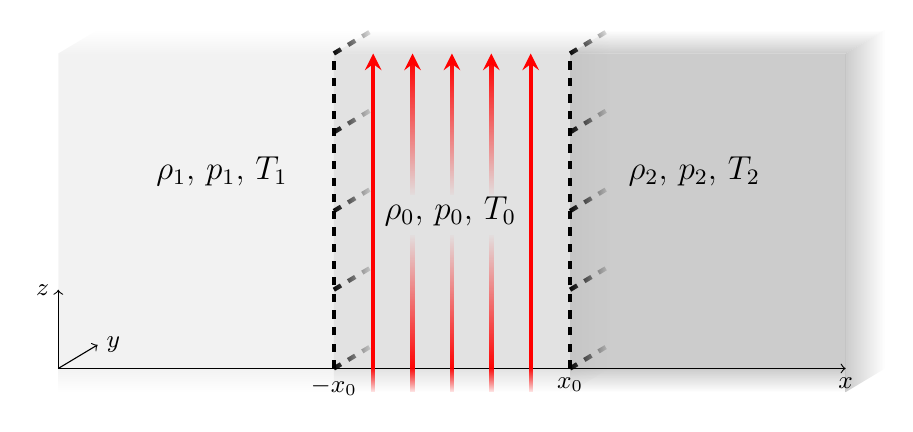
\begin{tikzpicture}
	\path [fill=lightgray, opacity=0.45] (3.5,0) -- (3.5,4) -- (6.5,4) -- (6.5,0) -- (3.5,0);
	\shade[left color=lightgray,right color=white, opacity=0.45] (6.5,0) -- (6.5,4) -- (7,4.3) -- (7,0.3) -- (6.5,0);
	\shade[top color=lightgray,bottom color=white, opacity=0.45] (3.5,0) -- (6.5,0) -- (6.5,-0.3) -- (3.5,-0.3) -- (3.5,0);
	\shade[top color=white,bottom color=lightgray, opacity=0.45] (3.5,4) -- (4,4.3) -- (7,4.3) -- (6.5,4) -- (3.5,4);
	\shade[left color=lightgray,right color=white, opacity=0.45] (6.5,0) -- (6.5,-0.3) -- (7,0) -- (7,0.3) -- (6.5,0);
	
	\path [fill=lightgray, opacity=0.8] (6.5,0) -- (6.5,4) -- (10,4) -- (10,0) -- (6.5,0);
	\shade[top color=lightgray,bottom color=white, opacity=0.8] (6.5,0) -- (10,0) -- (10,-0.3) -- (6.5,-0.3) -- (6.5,0);
	\shade[top color=white,bottom color=lightgray, opacity=0.8] (6.5,4) -- (7,4.3) -- (10.5,4.3) -- (10,4) -- (6.5,4);
	\shade[left color=lightgray,right color=white, opacity=0.8] (10,-0.3) -- (10,4) -- (10.5,4.3) -- (10.5,0) -- (10,-0.3);
	
	\path [fill=lightgray, opacity=0.2] (0,0) -- (0,4) -- (3.5,4) -- (3.5,0) -- (0,0);
	\shade[top color=lightgray,bottom color=white, opacity=0.2] (0,0) -- (3.5,0) -- (3.5,-0.3) -- (0,-0.3) -- (0,0);
	\shade[top color=white,bottom color=lightgray, opacity=0.2] (0,4) -- (0.5,4.3) -- (4,4.3) -- (3.5,4) -- (0,4);
	
	\draw [<->] (0,1) -- (0,0) -- (10,0);
	\draw [->] (0,0) -- (0.5,0.3);
	
	\draw [ultra thick, dashed] (3.5,0) -- (3.5,4);
	\draw [ultra thick, dashed, path fading=east] (3.5,0) -- (4,0.3);
	\draw [ultra thick, dashed, path fading=east] (3.5,4) -- (4,4.3);
	\draw [ultra thick, dashed, path fading=east] (3.5,2) -- (4,2.3);
	\draw [ultra thick, dashed, path fading=east] (3.5,1) -- (4,1.3);
	\draw [ultra thick, dashed, path fading=east] (3.5,3) -- (4,3.3);
	\draw [ultra thick, red, -stealth] (4,0) -- (4,4);
	\draw [ultra thick, red, path fading=south] (4,-0.3) -- (4,0);
	\draw [ultra thick, red, path fading=north] (4.5,0) -- (4.5, 1.7);
	\draw [ultra thick, red, path fading=south] (4.5,-0.3) -- (4.5,0);
	\draw [ultra thick, red, path fading=south] (4.5,2.2) -- (4.5,3.9);
	\draw [ultra thick, red, -stealth] (4.5,3.9) -- (4.5,4);
	\draw [ultra thick, red, path fading=north] (5,0) -- (5, 1.7);
	\draw [ultra thick, red, path fading=south] (5,-0.3) -- (5, 0);
	\draw [ultra thick, red, path fading=south] (5,2.2) -- (5,3.9);
	\draw [ultra thick, red, -stealth] (5,3.9) -- (5,4);
	\draw [ultra thick, red, path fading=north] (5.5,0) -- (5.5, 1.7);
	\draw [ultra thick, red, path fading=south] (5.5,-0.3) -- (5.5, 0);
	\draw [ultra thick, red, path fading=south] (5.5,2.2) -- (5.5,3.9);
	\draw [ultra thick, red, -stealth] (5.5,3.9) -- (5.5,4);
	\draw [ultra thick, red, -stealth] (6,0) -- (6,4);
	\draw [ultra thick, red, path fading=south] (6,-0.3) -- (6,0);
	\draw [ultra thick, dashed] (6.5,0) --(6.5,4);
	\draw [ultra thick, dashed, path fading=east] (6.5,0) -- (7,0.3);
	\draw [ultra thick, dashed, path fading=east] (6.5,4) -- (7,4.3);
	\draw [ultra thick, dashed, path fading=east] (6.5,2) -- (7,2.3);
	\draw [ultra thick, dashed, path fading=east] (6.5,1) -- (7,1.3);
	\draw [ultra thick, dashed, path fading=east] (6.5,3) -- (7,3.3);
	
	\small
	\node [below] at (3.5,0) {$-x_0$};
	\node [below] at (6.5,0) {$x_0$};
	\node [below] at (10,0) {$x$};
	\node [left] at (0,1) {$z$};
	\node [right] at (0.5,0.3) {$y$};
	
	\large
	\node [right] at (1.1,2.5) {$\rho_1$, $p_1$, $T_1$};
	\node [right] at (4,2) {$\rho_0$, $p_0$, $T_0$};
	\node [right] at (7.1,2.5) {$\rho_2$, $p_2$, $T_2$};
	\end{tikzpicture}
	\caption{The equilibrium state inside the slab, ($|x| \leq x_0$) and outside the slab, ($x < -x_0$ and $x > x_0$). The red arrows illustrate magnetic field lines, $B(x)\mathbf{\widehat{z}}$, and the dashed black lines indicate the boundaries of the slab. \textcolor{red}{Change to mag outside}}
	\label{fig:eq}
\end{figure}

To ensure that the model is in equilibrium, the total pressure in each external region must balance the total pressure in the internal region, namely
\begin{equation}
	p_1 + \frac{B_1^2}{2\mu_0} = p_0 + \frac{B_0^2}{2\mu_0} = p_2 + \frac{B_2^2}{2\mu_0}, \label{pressure balance}
\end{equation}
where $\mu_0$ is the permeability of free space. Defining the sound speed in each region by $c_j=\sqrt{\gamma p_j/\rho_j}$ for $j = 0, 1, 2$, where $\gamma$ is the adiabatic index\footnote{The adiabatic index is assumed uniform across the whole domain under the single-fluid approximation.}, we can rewrite Equation~\eqref{pressure balance} as
\begin{equation}
\rho_i\left(c_i^2 + \frac{\gamma}{2}v_{Ai}^2\right) = \rho_j\left(c_j^2 + \frac{\gamma}{2}v_{Aj}^2\right). \label{sound speeds}
\end{equation}


\subsection{The dispersion relation}

In the derivation of the dispersion relation, we decompose the linearised ideal MHD equations into Fourier forms then combine them into an ordinary differential equation (ODE) for the transverse velocity perturbation for each of the three plasma regions. After finding the general solution to each of these ODEs, we match the solutions across each interface at $\pm x_0$. The condition for the existence of non-trivial solutions will lead to the dispersion relation. In mathematical terms, we're converting a set of partial differential equations into ordinary differential equations into algebraic equations, into a single equation. From a form we cannot solve into a form we can.


\subsubsection{Derivation}

After linearising about a static equilibrium state, we can combine the governing equations and seek solutions of the form
\begin{equation}
\bv(\mathbf{x},t)=(\hat{v}_x(x)\textrm{e}^{i(kz-\omega{t})}, 0, \hat{v}_z(x)\textrm{e}^{i(kz-\omega{t})}),
\label{vcomponents}
\end{equation}
where $\mathbf{k} = (0, 0, k)$ is the wavenumber vector and $\omega$ is the angular frequency. This restricts the investigation to waves propagating parallel to the equilibrium magnetic field, with velocity perturbation amplitude $\hat{v}_x(x)$ in the $x$-direction, and $\hat{v}_z(x)$ in the $z$-direction. With this ansatz, the $x$ and $z$-components of the linearised momentum equation (Equation~\eqref{mom eqn lin}), describing the plasma dynamics within plasma region $j$, become
\begin{align}
&-\omega^2\hat{v}_x = (c_j^2+v_\textrm{Aj}^2)(\hat{v}_x'' + ik\hat{v}_z') - v_\textrm{Aj}^2ik\hat{v}_z'-v_\textrm{Aj}^2k^2\hat{v}_x, \label{I} \\
&-\omega^2\hat{v}_z = c_j^2ik(\hat{v}_x' + ik\hat{v}_z), \label{J}
\end{align}
where $v_\textrm{Aj}$ is the Alfv\'{e}n speed in region $j$ and $'=\textrm{d}/\textrm{d}x$. These equations can be combined to give an ordinary differential equation for $\hat{v}_x$, namely
\begin{equation}
\hat{v}_x'' - m_j^2\hat{v}_x = 0, \quad \text{where} \quad
m_j^2 = \frac{(k^2v_\textrm{Aj}^2 - \omega^2)(k^2c_j^2 - \omega^2)}{(c_j^2 + v_\textrm{Aj}^2)(k^2c_\textrm{Tj}^2 - \omega^2)}, \label{O}
\end{equation}
where $j = 0, 1, 2$. This is identical to the corresponding equation for a symmetric slab derived by \cite{rob81c}.

Solutions of Equations~\eqref{O} and~\eqref{P} are a linear combination of hyperbolic functions. We restrict our model to waves trapped by the slab by imposing the boundary condition $\hat{v}_x \to 0$ as $|x| \to \infty$. Thus, the general solution for the velocity perturbation in the $x$-direction is
\begin{equation}
\hat{v}_x(x)=
\begin{cases}
A(\cosh{m_1x} + \sinh{m_1x}), & \text{if } x < -x_0, \\
B\cosh{m_0x} + C\sinh{m_0x}, & \text{if } |x| \leq {x_0}, \\
D(\cosh{m_2x} - \sinh{m_2x}), & \text{if  } x > x_0, 
\end{cases} \label{vsoln}
\end{equation}
where $A$, $B$, $C$, and $D$ are arbitrary constants (with respect to $x$). The plasma pressure perturbation can be assumed to be of the form $p(\mathbf{x},t)=\hat{p}(x)e^{i(kz - \omega t)}$, then the perturbation in total pressure (plasma pressure plus magnetic pressure) across the whole domain has amplitude
\begin{equation}
\hat{P}(x) = \hat{v}_x'(x)
\begin{cases}
\Lambda_1/m_1, & \text{if } x < -x_0, \\
\Lambda_0/m_0, & \text{if } |x| \leq x_0, \\
\Lambda_2/m_2, & \text{if } x > x_0,
\end{cases}
\end{equation}
where
\begin{equation}
\Lambda_j=-\frac{i\rho_j(k^2v_\textrm{Aj}^2 - \omega^2)}{m_j\omega}. \label{Lambdas}
\end{equation}
The remaining boundary conditions are continuity of velocity and total pressure across the slab boundaries at $x = \pm{x_0}$, which gives the four coupled homogeneous algebraic equations
\begin{equation}
\left(
\begin{matrix}
c_1-s_1             &-c_0           &s_0            &0                   \\
0                   &c_0            &s_0            &s_2-c_2             \\
\Lambda_1(c_1-s_1)  &\Lambda_0s_0  &-\Lambda_0c_0   &0                   \\
0                   &\Lambda_0s_0  &\Lambda_0c_0  &-\Lambda_2(s_2-c_2)
\end{matrix}
\right)
\left(
\begin{matrix}
A \\
B \\
C \\
D
\end{matrix}
\right)
=
\left(
\begin{matrix}
0 \\
0 \\
0 \\
0
\end{matrix}
\right),
\label{coefmatrix}
\end{equation}
where $c_j = \cosh{m_jx_0}$ and $s_j = \sinh{m_jx_0}$ for $j=0,1,2$, for brevity. The condition for the existence of non-trivial solutions to this system of equations is that the determinant of the matrix is zero. Applying this condition gives us the dispersion relation for an asymmetric slab, namely
\begin{equation}
(\Lambda_0^2 + \Lambda_1\Lambda_2) + \Lambda_0(\Lambda_1 + \Lambda_2)\coth{2m_0x_0} = 0. \label{DR lambda}
\end{equation}
By expanding $\Lambda_j$, we can write this as
\begin{align}
&m_0^2(k^2v_{A1}^2 - \omega^2)(k^2v_{A1}^2 - \omega^2) + \frac{\rho_0}{\rho_1}m_1\frac{\rho_0}{\rho_2}m_2(k^2v_\textrm{A0}^2 - \omega^2)^2 \notag \\
& + m_0(k^2v_\textrm{A0}^2-\omega^2)\left[\frac{\rho_0}{\rho_1}m_1(k^2v_{A2}^2 - \omega^2) + \frac{\rho_0}{\rho_2}m_2(k^2v_{A1}^2 - \omega^2)\right]\coth{2m_0x_0} = 0. \label{DR}
\end{align}


\subsubsection{First-order symmetric slab}

There is an intrinsic difference between perturbations along symmetric and asymmetric magnetic slabs. The dispersion relation governing an asymmetric slab is a single equation, whereas the dispersion relation governing a symmetric slab \citep{rob81a} consists of two independent equations, corresponding to the sausage and kink eigenmodes.

Under the approximation that the densities and temperatures of the external plasma are of the same order, the dispersion relation, Equation~\eqref{DR}, can be factorised to give the approximate dispersion relation
\begin{equation}
\left[\Lambda_0(\Lambda_1+\Lambda_2)+2\Lambda_1\Lambda_2\tanh{m_0x_0}\right]\left[\Lambda_0(\Lambda_1+\Lambda_2)+2\Lambda_1\Lambda_2\coth{m_0x_0}\right]=0.
\end{equation}
To show this, define each bracket as the following functions
\begin{align}
D_k(\omega) &:= \Lambda_0 (\Lambda_1 + \Lambda_2) + 2\Lambda_1\Lambda_2\coth{m_0x_0}, \\
D_s(\omega) &:= \Lambda_0(\Lambda_1 + \Lambda_2) + 2\Lambda_1\Lambda_2\tanh{m_0x_0}.
\end{align}
There product is then
\begin{align}
D_k(\omega) D_s(\omega) &= \left[ \Lambda_0 (\Lambda_1 + \Lambda_2) + 2\Lambda_1\Lambda_2\coth{m_0x_0} \right] \left[ \Lambda_0(\Lambda_1 + \Lambda_2) + 2\Lambda_1\Lambda_2\tanh{m_0x_0} \right] \\
&= \Lambda_0^2 (\Lambda_1 + \Lambda_2)^2 + 2\Lambda_0(\Lambda_1 + \Lambda_2)\Lambda_1\Lambda_2(\tanh{m_0x_0} + \coth{m_0x_0}) + 4\Lambda_1^2\Lambda_2^2 \\
&= 4\Lambda_1\Lambda_2 \left[ (\Lambda_0^2F + \Lambda_1\Lambda_2) + \Lambda_0(\Lambda_1 + \Lambda_2)\coth(2m_0x_0) \right] \\
\end{align}
where
\begin{equation}
F = \frac{(\Lambda_1 + \Lambda_2)^2}{4\Lambda_1\Lambda_2},
\end{equation}
which, when the conditions on each side of the slab are approximately symmetric, \textit{i.e.} $\Lambda_2 = \Lambda_1 (1 + \epsilon L)$, with $\epsilon \ll 1$ and $L \approx 1$, becomes
\begin{equation}
F = \frac{(2 + \epsilon L)^2}{4(1 + \epsilon L)} = 1 + \mathcal{O}(\epsilon^2).
\end{equation}
Therefore, 
\begin{align}
D(\omega) &= (\Lambda_0^2 + \Lambda_1\Lambda_2) + \Lambda_0(\Lambda_1 + \Lambda_2)\coth(2m_0x_0), \\
&= \frac{1}{4\Lambda_1\Lambda_2} D_k(\omega) D_s(\omega) + \mathcal{O}(\epsilon^2).
\end{align}
Therefore, to linear order, the approximate dispersion relation is satisfied if the waveguide asymmetry is small.

The expressions for the variables $\Lambda_i$ for $i=0,1,2$ in Equations~\eqref{Lambdas} can be employed to yield the approximately symmetric dispersion relation
\begin{equation}
(k^2v_\textrm{A0}^2-\omega^2)\left(\frac{\rho_0}{\rho_1}\frac{m_1}{(k^2v_\textrm{A1}^2-\omega^2)} + \frac{\rho_0}{\rho_2}\frac{m_2}{k^2v_\textrm{A2}^2-\omega^2}\right) + 2m_0\left(\begin{matrix}\tanh \\ \coth \end{matrix}\right)(m_0x_0) = 0. \label{DRapprox}
\end{equation}
This equation is now in an analogous form to the dispersion relation corresponding to MHD waves along a symmetric magnetic slab \citep{rob81b}, namely
\begin{equation}
(k^2v_\textrm{A}^2-\omega^2)\frac{\rho_0}{\rho_\textrm{e}}m_\textrm{e}=\omega^2m_0\left(\begin{matrix}\tanh \\ \coth \end{matrix}\right)(m_0x_0), \label{DRsym}
\end{equation}
where external parameters are denoted by subscript $\textrm{e}$.


%------------------------------------------------------------------------------
\section{Asymmetric slab in a non-magnetic environment}
\label{sec: EVP non-mag}
%------------------------------------------------------------------------------

By letting $B_1 = B_2 = 0$, the plasma in the external regions is non-magnetic.

\subsection{Analytical solutions}

\subsubsection{Spurious solutions}

\subsubsection{Limiting case - incompressible plasma}

\subsubsection{Limiting case - zero-beta}

\subsubsection{Limiting case - thin slab}

\subsubsection{Limiting case - wide slab}

\subsection{Numerical solutions}

\subsubsection{Varying the degree of asymmetry}

\subsection{Eigenfunctions}

\subsubsection{Analogy to coupled spring and mass oscillator}
Actually do the maths for this.


%------------------------------------------------------------------------------
\section{Asymmetric slab in a magnetic environment}
\label{sec: EVP mag}
%------------------------------------------------------------------------------

\subsection{Model description}

\subsection{The dispersion relation}

\subsection{Implications for observations}

\subsubsection{Quasi-symmetric modes}

\subsubsection{Asymmetric mode or superposition of symmetric modes?}
Table of observable indicators of each case.

\subsubsection{Possible alternative causes of observed asymmetry}
Possibilities: 
\begin{itemize}
	\item Asymmetric ICs
	\item Non-collective oscillations
	\item Observational artefact
\end{itemize}
Include discussion about how to differentiate between these.



\bibliographystyle{plainnat}
\bibliography{../main/references}  

\end{document}


%------------------------------------------------------------------------------
\chapter{Ray theory}
\label{chap: ray}
%------------------------------------------------------------------------------

%------------------------------------------------------------------------------
\section{Chapter introduction}
\label{sec: ray intro}
%------------------------------------------------------------------------------

	In this section, we give an introduction to MHD ray theory, use ray theory to characterise guided and leaky modes of MHD waveguides, and provide an alternative derivation of the dispersion relation for MHD slab waveguides. The significance of this approach is that it could present a method of deriving a dispersion relation in cases where the differential equation approach is intractable.
	
	Ray theory (also known as ray optics or geometric optics) is an approach to studying wave propagation that models waves as continuous lines, known as \textit{rays}. It is extensively used in electromagnetic wave theory but has largely been neglected in MHD and solar physics. It provides a mathematically tractable description of phenomena such as reflection and refraction, but is inadequate to describe phenomena such as diffraction which require a wave-based approach.
	
	Due to the dominance of its use in electromagnetism, ray theory is mostly encountered in isotropic media, that is, media for which wave propagation is independent of propagation direction. While MHD wave propagation is inherently anisotropic due to the magnetic field, isotropic ray theory remains instructive for MHD because some limiting cases in MHD exhibit isotropic wave propagation.
	
	The seminal text for ray theory is \cite{bor_etal99}, which covers electromagnetic wave propagation in both isotropic and anisotropic media. Also, \cite{vei_etal10} gives a particularly intuitive description of electromagnetic wave propagation in uniaxial crystals which demonstrates the type of optical anisotropy that is a most similar to MHD media. The authors define a crystal axis is a direction along which propagating light suffers no birefringent, that is, rays are refracted in one, rather than many, direction. Uniaxial crystals are crystals which have one crystal axis. Light propagation along the plane perpendicular to the single crystal axis in a uniaxial crystal is isotropic. In this sense, the magnetic field direction is to MHD waves as the crystal axis is to light waves. 
	
	The slab waveguide, the centrepiece of this thesis, is a prototypical model for guiding electromagnetic waves. The electromagnetic slab waveguide is formed by dielectric layers and is used in, for example, integrated optical circuits and optical fibres \citep{ram_etal84}. Modes analogous to MHD body modes, that is, modes which are spatially oscillatory within the waveguide, are guided by right-handed electromagnetic slabs. They are termed \textit{right-handed} because the electric field vector, magnetic field vector, and wavevector form a right-handed orthogonal set \citep{ram_etal84}. Modes analogous to MHD surface modes, that is, modes that are evanescent within the waveguide where the wave energy is confined to the interfaces, are guided by left-handed electromagnetic slabs \citep{wan_etal08,ash13,sha_etal03}. Left-handed optical waveguides are more esoteric than right-handed optical waveguides because of the engineering complexity of meta-materials that are required to construct such waveguides.
	
	\cite{Hu_etal09} give an overview of the theory and applications of electromagnetic slab waveguides. They focus on leaky modes, giving a particularly intuitive description of energy leakage as the result of partial internal reflection leading to energy being transmitted to the external region. Minimising energy leakage is key to avoiding energy losses in optical communication infrastructure. They also expand the theory of the W-type slab waveguide, which is constructed by two adjacent slab waveguides. \cite{mar74} generalises the theory of optical slab waveguides to an asymmetric slab, analogous to the asymmetric slab MHD waveguide modelled in this thesis.
	
	Severe inhomogeneities exists across a broad range of length scales in the solar atmosphere, from the global scale at the transition region between the chromosphere and the corona, to the smallest scales that we can currently resolve in magnetic bright points in inter-granular lanes. When waves are incident on these structures, the wave's energy is partially reflected and partially transmitted, with the remainder of the energy dissipated into the background plasma or converted to a different MHD wave mode. Ray theory is an appropriate model for the reflection and transmission of MHD waves.
	
	The basic theory of MHD ray theory has been established for some time. \cite{mck70} calculated the reflection and transmission coefficients for MHD waves incident on the magnetopause. \cite{ver73} extended this by calculating the transmitted energy and \cite{wol_etal75} comparing to instances of large perturbations of the magnetopause by oscillations in the solar wind. The ray theory behind these results is particularly well explained by \cite{wal04}. Nonlinear MHD ray theory has recently been investigated by \cite{nun18} and \cite{nun20}.
	
	MHD waves have long been a considered mechanism for plasma heating. Wave eating of plasma in the Sun's corona would require energy to be efficiently transported from the solar interior and dissipated at a given height, but there is no wave mode that is both efficient at energy transportation and energy dissipation. One possibility is that mode conversion occurs between a mode with efficient energy transportation to a mode with efficient energy dissipation \citep{par_etal12}. To incorporate mode conversion to MHD ray theory, \cite{shu_etal06} developed a \textit{generalized ray theory}. This theory has also been used in helioseismology. \cite{cal06} numerically investigated the mode conversion of MHD waves in the Sun's interior at the position of equipartition between the sound and Alfv\'{e}n speeds and the acoustic cut-off position.
	
	\cite{lee_etal02a} utilise a numerical method known as \textit{invariant embedding} to solve a system of nonlinear boundary value differential equations to derive expressions for the reflection and transmission coefficients (that is, the amplitude modulation factor that a wave undergoes upon reflection or transmission) of MHD waves when propagating through arbitrary non-uniform regions. They then use this to derive a relationship between the reflection and transmission coefficients (that is, the amplitude modulation factor that a wave undergoes upon reflection or transmission) and the damping time of MHD waves.
	
	Using ray theory of MHD waves normally incident on a multi-layered plasma model of the interface between the solar wind and Earth's magnetosphere, \cite{leo_etal03} estimated that 40\% of the wave energy flux incident on the magnetosphere is transmitted into the magnetosphere. This is enough to explain the energy in moderate geomagnetic sub-storms.
	
	This chapter uses ray theory to determine the discrete spectrum of eigenfrequencies of MHD waveguides. This is manifested by imposing the condition that rays that are internally reflected from the boundaries of the waveguide must have equal phase to rays that travel the same distance without reflection. This technique has been employed in standard electromagnetic ray theory \citep{bor_etal99}. In MHD, it has been explored for simple waveguides such as a symmetric slab waveguide modelling waves guided by a coronal hole \citep{dav_85}.
	
	
	%------------------------------------------------------------------------------
	\section{Anisotropic ray theory}
	\label{sec: aniso ray}
	%------------------------------------------------------------------------------
		
	There are two notions of a wave's direction: phase velocity and group velocity. The phase velocity, $\mathbf{v_{ph}} = \omega / |k| \mathbf{\widehat{k}}$ is the velocity with which each peak and trough travels and the group velocity, $\mathbf{v_g} = \partial \omega / \partial \mathbf{k}$, is the velocity with which the envelope of a wave packet travels. In general, these directions are different. However, in the ray theory of isotropic media, there is an unambiguous notion of direction of the wave. This can be proven as follows.
	
	Using the quotient rule, we can show that the group and phase velocities are related by
	\begin{equation}
	\mathbf{v_g} = \mathbf{v_{ph}} + k\nabla_k v_{ph}, \label{group vel}
	\end{equation}
	where $v_{ph} = |\mathbf{v_{ph}}|$ and $\nabla_k = (\partial/\partial k_x, \partial/\partial k_y)$. Let's restrict the domain to the $xy$-plane for ease of algebra and define the angle that $\mathbf{k}$ makes with the $x$-axis to be $\theta$. Now, by the chain rule,
	\begin{equation}
	\frac{\partial}{\partial \theta} = -k_y \frac{\partial}{\partial k_x} + k_x \frac{\partial}{\partial k_y}.
	\end{equation}
	Therefore, taking the magnitude of the cross product of Equation~\eqref{group vel} with $\mathbf{k}$ leads to
	\begin{equation}
	|\mathbf{k} \times \mathbf{v_g}| = \frac{\partial v_{ph}}{\partial \theta}.
	\end{equation}
	Therefore, if the medium is isotropic, \textit{i.e.} if the right-hand side of the above equation is zero, then the group velocity is parallel to $\mathbf{k}$ and hence is parallel to the phase velocity, which concludes the proof. The proof for a general three-dimensional domain is similar but each direction is uniquely determined by two angles, rather than one.
	
	When the medium is anisotropic, then the phase speed is dependent on the angle of propagation, therefore is is possible for the group speed to have a component perpendicular to the phase speed (see Figure~\ref{fig: anisotropic ray direction}).
	\begin{figure}
		\centering
		\includegraphics[width=0.7\textwidth]{\figdirIII ray.eps}
		\caption{In an anisotropic fluid, wave packets and wavefronts can travel in different directions.}
		\label{fig: anisotropic ray direction}
	\end{figure}
	For anisotropic ray theory, a natural question to ask is: along which direction does the ray travel? The answer to this is dependent on the purpose. Of course, ray theory is merely a model of reality; its importance is in virtue of its utility rather than its truthfulness, \textit{per se}. So we are free to choose which is most useful. Ray theory using the phase direction, \textit{i.e.} the direction normal to wavefronts, is known as \textit{geometric optics} and ray theory using the group direction, \textit{i.e.} the direction along which the wave energy propagates, is known as \textit{Hamiltonian optics}. For our purpose, which is to derive the dispersion relation for guided MHD waves, we will be required to impose a condition of matching the phase of two reflected waves. This motivates the use of the phase direction for MHD rays. Therefore, geometrical optics is more suitable for the present purpose. This disambiguation is laid out more fully for electromagnetic ray theory by \cite{has88} and for MHD ray theory by \cite{wal77}.
	
	A third characteristic speed is the \textit{ray velocity}, which is the speed of the energy ray, defined by $v_r = v_{ph}/\cos{\alpha}$, where $\alpha$ is the angle between the group velocity and the phase velocity. In other words, the ray velocity is the component of the phase velocity parallel to the group velocity. For an isotropic fluid, $\alpha = 0$, therefore making the ray velocity equal to the phase velocity.
	
	A key principle for ray theory is Fermat's Principle of Least Time, which states that the path taken by an energy ray between two points is that which takes least time for the ray to cover. We can use this to define the energy ray path. Then we can use this definition to determine a relationship between the phase angles of incident, reflection, and transmitted rays when a ray is incident on a planar interface as follows.
	
	\begin{figure}
		\centering
		\includegraphics[width=0.7\textwidth]{\figdirIII snell.eps}
		\caption{An isotropic ray is incident on a planar interface between two plasmas with refractive indices $n_1$ and $n_2$, respectively. The energy ray path is from point $A$ to $B$ via $O$. The phase ray path, which propagates at an angle $\alpha$ to the energy ray path, is from point $A$ to $B'$ via $O'$. The phase ray path makes an angle of $\theta_1$ with the interface.}
		\label{fig: fermat}
	\end{figure}
	
	Fermat's principle applied to paths connecting points $A$ and $B$ can be written as
	\begin{equation}
	\delta T = \delta \int_A^B \frac{1}{v_r} ~ds = 0,
	\end{equation}
	where $s$ is the arc length measured along the path from $A$ to $B$ and $T$ is the time for the energy ray to travel between $A$ and $B$ \citep{bor_etal99}. The symbol $\delta$ denotes a small change in a quantity. When the domain is divided by an interface parallel to the $z$-axis, with uniform plasma on each side, making a change of variables $p = s \cos{\alpha}$ leads to $dp = \cos{\alpha} ~ds$ in each uniform region. Therefore, 
	\begin{equation}
	T = \int_A^O \frac{1}{v_r} ~ds + \int_O^B \frac{1}{v_r} ~ds = \int_A^{O'} \frac{1}{v_{ph}} ~dp + \int_{O'}^{B'} \frac{1}{v_{ph}} ~dp,
	\end{equation}
	which has effectively changed the contour of the integral from the energy ray path to the phase ray path. Using the notation defined in Figure~\ref{fig: fermat}, $T$ can be written as
	\begin{equation}
	T = \frac{\sqrt{z^2 + a^2}}{v_{ph1}} + \frac{\sqrt{b^2 + (s-z)^2}}{v_{ph2}}.
	\end{equation}
	Each region in homogeneous, so the ray is a straight line in each region. Therefore,
	\begin{equation}
	\frac{dT}{dz} = \frac{z}{v_{ph1}\sqrt{z^2 + a^2}} - \frac{s - z}{v_{ph2}\sqrt{b^2 + (s - z)^2}}.
	\end{equation}
	By noticing that
	\begin{equation}
	\cos{\theta_1} = \frac{z}{\sqrt{z^2 + a^2}} \quad \text{and} \quad \cos{\theta_2} = \frac{s - z}{\sqrt{b^2 + (s - z)^2}},
	\end{equation}
	we can write
	\begin{equation}
	\frac{dT}{dz} = \frac{1}{v_{ph1}}\cos{\theta_1} - \frac{1}{v_{ph2}}\cos{\theta_2}.
	\end{equation}
	By Fermat's Principle, this must vanish, hence,
	\begin{equation}
	\frac{1}{v_{ph1}}\cos{\theta_1} = \frac{1}{v_{ph2}}\cos{\theta_2}. \label{snell}
	\end{equation}
	This is Snell's law, which we have shown to still hold for the phase ray in anisotropic media.
	
	If we instead position point $B$ (and hence point $B'$) on the same side of the interface as point $A$, then Equation~\eqref{snell} reduces to $\theta_i = \theta_r$, known as the \textit{Law of Reflection}, which we have shown holds for the phase ray. Snell's law does not hold for the energy ray but the law of reflection does.
	
	
	%------------------------------------------------------------------------------
	\section{Low-beta ray theory of a slab waveguide}
	\label{sec: low beta}
	%------------------------------------------------------------------------------
	
	In general, magneto-acoustic waves are anisotropic, that is, they propagate with different speed depending on their propagation angle. The phase speeds of fast and slow magneto-acoustic waves are given by
	\begin{equation}
	v_\mathrm{ph}^2 = \frac{\omega^2}{k^2} = \frac{1}{2}\left[ (v_A^2 + c_0^2) \pm \sqrt{(v_A^2 + c_0^2)^2 - 4v_A^2c_0^2\frac{k_z^2}{k^2}} \right]. \label{MHD DR}
	\end{equation}
	When kinetic pressure is negligible compared to the magnetic pressure, \textit{i.e.} $v_A \gg c_0$, then the fast speed is approximately $v_A$, and the slow speed is approximately $0$. That is, the fast mode propagates isotropically at the Alfv\'{e}n speed and the slow mode degenerates. Clearly, the group velocity is also $\mathbf{v_g} = v_A \mathbf{\widehat{k}}$, where $\mathbf{\widehat{k}} = \mathbf{k}/k$, so is equal to the phase velocity. Hence, there is an unambiguous ray direction. Therefore, the ray theory of isotropic optical waveguides is isomorphic to low-beta MHD ray theory.
	
	Consider an asymmetric slab MHD waveguide of low-beta plasma. Since MHD wave propagation in low-beta plasma is isotropic, the dispersion relation for guided low-beta MHD waves along an asymmetric slab can be derived in the same way as for guided electromagnetic waves in an asymmetric dielectric slab waveguide. The derivations differ only by notation.
	
	\cite{ram_etal84} used ray theory to show that the eigenfrequencies, $\omega$, of (transverse electric mode\footnote{In general, guided electromagnetic waves propagate in a superposition of transverse electric modes and transverse magnetic modes. The transverse electric modes have no electric field in the direction of propagation, and the transverse magnetic modes have no magnetic field in the direction of propagation. The transverse electric mode is analogous to the MHD modes due to their polarisation with respect to the slab boundaries.}) electromagnetic waves guided by an asymmetric dielectric waveguide satisfy the dispersion relation (their Equation~7 in Chapter~14.7)
	\begin{equation}
	\tan{hd} = \frac{h(q + p)}{h^2 - pq}, \label{EM DR}
	\end{equation}
	where $d$ is the width of the waveguide, waves propagate in proportion to $e^{i\beta z}$ in the $z$-direction, and\footnote{Note that we have changed the subscripts to be in keeping with the notation in this thesis.} 
	\begin{equation}
	q^2 := \beta^2 - k_1^2, \quad h^2 := k_0^2 - \beta^2, \quad p^2 := \beta^2 - k_2^2.
	\end{equation}
	The rays in each dielectric medium $i$ travel at speed $\omega/k_i = v_i$. Therefore, $q^2 = \beta^2 - \omega^2/v_1^2$, $h^2 = \omega^2/v_0^2 - \beta^2$, and $p^2 = \beta^2 - \omega^2/v_2^2$. Therefore, Equation~\eqref{EM DR} is equivalent to
	\begin{equation}
	\Lambda_0(\Lambda_1 + \Lambda_2) + (\Lambda_0^2 + \Lambda_1\Lambda_2)\tanh{d\Lambda_0} = 0, \label{EM DR 2}
	\end{equation}
	where $\Lambda_i = \sqrt{\beta^2 - \omega^2/v_i^2}$ and we have used $\tan{i\theta} = i \tanh{\theta}$. Equation~\eqref{EM DR 2} is isomorphic to the dispersion relation for guided low-beta MHD modes (see \citealp{all_etal17}) of an asymmetric slab by setting the phase speeds of the rays to be the Alfv\'{e}n speed, $v_i = v_{Ai}$, for $i = 0, 1, 2$.
	
	
	%------------------------------------------------------------------------------
	\section{Finite-beta ray theory of a slab waveguide}
	\label{sec: finite beta}
	%------------------------------------------------------------------------------
	
	Next, we relax the low-beta condition. This allows for anisotropic wave propagation. This is most clearly illustrated in the Friedrichs diagrams which demonstrate how the phase and group speeds of MHD waves depend on the angle of propagation (see, for example, \citealp{goe_etal04,pri14}). In this section, we use MHD ray theory to derive the dispersion for an asymmetric slab.
	
	Consider a small-amplitude magnetoacoustic phase ray propagating incident on the interface between plasma regions 0 and 2 at an angle of $\theta_i$. The velocity perturbation associated with this incident wave can be written $\mathbf{v_i} = (v_{ix}, 0, v_{iz})$ as we have already shown that the magnetoacoustic modes have no component perpendicular to the magnetic field and parallel to the slab boundaries. Only the Alfv\'{e}n mode perturbs the plasma in this direction, and that mode is decoupled from the magnetoacoustic modes. In general, the incident ray will be partially reflected and partially transmitted. Each of these waves can be decomposed into a linear superposition of plane waves, whose transverse velocity components have the form
	\begin{align}
	v_{ix} &= \widehat{v}_{ix} e^{i(\mathbf{k_i}\cdot \mathbf{x} + \omega t)}, \\
	v_{rx} &= \widehat{v}_{rx} e^{i(\mathbf{k_r}\cdot \mathbf{x} - \omega t)}, \\
	v_{tx} &= \widehat{v}_{tx} e^{i(\mathbf{k_t}\cdot \mathbf{x} - \omega t)},
	\label{fourier}
	\end{align}
	where subscripts $i, r, t$ refer to the \textit{incident}, \textit{reflected}, and \textit{transmitted} waves. Let the angles that the incident, reflected, and transmitted rays make with the interface be $\theta_i$, $\theta_r$, and $\theta_t$, respectively.
	
	The interfaces between the plasmas are free surfaces with tangential magnetic field, so the dynamic and kinematic boundary conditions are equivalent to the normal velocity component and total pressure perturbation being continuous at the interface \citep{goe_etal04}. Continuity of normal velocity at $x = 0$ gives
	\begin{equation}
	\widehat{v}_{ix}e^{i(k_{iz}z - \omega t)} + \widehat{v}_{rx}e^{i(k_{rz}z - \omega t)} = \widehat{v}_{tx}e^{i(k_{tz}z - \omega t)}. \label{norm vel 1}
	\end{equation}
	The Law of Reflection tells us that $\theta_r = \theta_i$. The incident, reflected, and transmitted ways must have equal phase at the interface $x = 0$, known as the phase matching condition. This implies that the frequency on each side must be equal. Thus, Snell's Law tells us that the tangential components of the wave-vector components obey
	\begin{equation}
	k_i\cos{\theta_i} = k_r\cos{\theta_r} = k_t\cos{\theta_t}. \label{tang comp}
	\end{equation}
	Therefore, by the Law of Reflection $k_r = k_i$. In particular, $k_{rx} = -k_{ix}$ and $k_{rz} = k_{iz}$. Therefore, Equation~\eqref{norm vel 1} reduces to
	\begin{equation}
	\widehat{v}_{ix} + \widehat{v}_{rx} = \widehat{v}_{tx}. \label{cont vel}
	\end{equation}
	
	The total pressure perturbation for a ray with wave-vector $\mathbf{k} = (k_x, 0, k_z)$ is derived as follows. The linearised perturbation in magnetic pressure is $p_m = B_0b_{iz}/\mu_0$, where $B_0$ and $b_{iz}$ are the equilibrium and $z$-component of the magnetic field in the slab region and $\mu_0$ is the magnetic permeability. Using the $z$-component of the induction equation,
	\begin{equation}
	\widehat{b}_{iz} = \frac{B_0}{\omega}k_{ix}\widehat{v}_x, \label{ind eq z}
	\end{equation}
	where $b_{iz} = \widehat{b}_{iz} e^{i(\mathbf{k_i}\cdot \mathbf{x} + \omega t)}$. The energy and continuity equations can be combined to
	\begin{equation}
	\frac{\partial p}{\partial t} = - \rho_0 c_0^2 \nabla \cdot \mathbf{v}.
	\end{equation}
	A Fourier decomposition of this equation yields
	\begin{equation}
	\widehat{p} = -\frac{\rho_0c_0^2}{\omega} (k_x\widehat{v}_x + k_z\widehat{v}_z). \label{pressure eq}
	\end{equation}
	The $z$-component of the momentum equation is
	\begin{equation}
	\frac{\partial^2 v_z}{\partial t^2} = c_0^2 \frac{\partial}{\partial z}(\nabla \cdot \mathbf{v}),
	\end{equation}
	which, when taking Fourier forms, reduces to
	\begin{equation}
	\widehat{v}_z = - \frac{ic_0^2k_z}{k_zc_0^2 - \omega^2}k_x\widehat{v}_x. \label{vx vz}
	\end{equation}
	Equations~\eqref{ind eq z},~\eqref{pressure eq}, and~\eqref{vx vz} combine to give an expression for the total pressure perturbation, namely
	\begin{equation}
	\widehat{p}_T = \widehat{p} + \widehat{p}_m = \frac{\Lambda_0}{m_0}ik_x\widehat{v}_x,
	\end{equation}
	where, as defined in \cite{all_etal17},
	\begin{equation}
	\Lambda_j = \frac{i\rho_j(\omega^2 - k_z^2v_{Aj}^2)}{\omega m_j}, \quad m_j^2 = \frac{(k_z^2 v_{Aj}^2 - \omega^2)(k_z^2 c_{j}^2 - \omega^2)}{(c_j^2 + v_{Aj}^2)(k_z^2 c_{Tj}^2 - \omega^2)}.
	\end{equation}
	Equation~\eqref{MHD DR} can be rearranged to give
	\begin{equation}
	k_x^2 = -\frac{(k_z^2 v_{A0}^2 - \omega^2)(k_z^2 c_{0}^2 - \omega^2)}{(c_0^2 + v_{A0}^2)(k_z^2 c_{T0}^2 - \omega^2)}.
	\end{equation}
	Therefore, $k_{rx} = -k_{ix} = -im_0$ and $k_{tx} = im_2$. Hence, the condition of continuity of total pressure at the interface is equivalent
	\begin{equation}
	\Lambda_0(\widehat{v}_{ix} - \widehat{v}_{rx}) = \Lambda_2 \widehat{v}_{tx}. \label{cont pressure}
	\end{equation}
	Equations~\eqref{cont vel} and~\eqref{cont pressure} can be solved simultaneously to find
	\begin{align}
	\widehat{v}_{ix} &= \frac{1}{2}\widehat{v}_{tx}\left(1 + \frac{\Lambda_2}{\Lambda_0}\right) \\
	\widehat{v}_{rx} &= \frac{1}{2}\widehat{v}_{tx}\left(1 - \frac{\Lambda_2}{\Lambda_0}\right).
	\end{align}
	The ratio of these is the reflection coefficient, namely
	\begin{equation}
	r_2 := \frac{\widehat{v}_{rx}}{\widehat{v}_{ix}} = \frac{\Lambda_0 - \Lambda_2}{\Lambda_0 + \Lambda_2}. \label{reflection coefficient}
	\end{equation}
	
	Total internal reflection occurs for $\theta_i < \theta_c$, where $\cos{\theta_c} = k_t / k_i$. In this case,
	\begin{align}
	k_{tx}^2 &= k_t^2 \sin^2{\theta_t} \\
	&= k_t^2(1 - \cos^2{\theta_t}) \\
	&= k_t^2 - k_i^2\cos^2{\theta_i} \\
	&< k_t^2 - k_i^2\cos^2{\theta_c} \\
	&= k_t^2 - k_i^2 \left(\frac{k_t^2}{k_i^2}\right) \\
	&= 0.
	\end{align}
	Therefore, $k_{tx}$, and hence $\Lambda_2$, is imaginary. Therefore, define $L_2$ by $\Lambda_2 = i L_2$, with $L_2 \in \mathbb{R}$ so that we can write
	\begin{equation}
	r_2 = \frac{\Lambda_0 - iL_2}{\Lambda_0 + iL_2}. \label{reflection coefficient 2}
	\end{equation}
	The variable $\Lambda_0$ can be real or imaginary. First, we consider the case when $\Lambda_0$ is real.
	
	
	\subsection{Body modes}
	When $\Lambda_0$ is real, $k_{ix}$ is real, therefore Equation~\eqref{fourier} tells us that this corresponds to spatially oscillatory (rather than evanescent) incident rays. It will become clear that this necessitates guided body modes.
	
	In this case, $r_2$ is complex. In accordance with ray theory theory, the real part gives the ratio of amplitudes of the reflected and incident rays, and the imaginary part gives a phase shift that the incident ray undergoes upon reflection \citep{bor_etal99}. The reflection coefficient $r_2$ given by Equation~\eqref{reflection coefficient 2} has complex argument
	\begin{equation}
	\phi_2 = -2 \arctan\left(\frac{L_2}{\Lambda_0}\right).
	\end{equation}
	This is the phase shift that the incident ray undergoes after total internal reflection on the interface between plasma 0 and 2. Similarly, the phase shift that an incident ray undergoes after total internal reflection on the interface between plasma 0 and 1 is
	\begin{equation}
	\phi_1 = -2 \arctan\left(\frac{L_1}{\Lambda_0}\right).
	\end{equation}
	
	\begin{figure}
		\centering
		\includegraphics[width=\textwidth]{\figdirIII ray-slab.pdf}
		\caption{Ray paths (dashed) travelling in an asymmetric slab made up of three plasma regions of different refractive indices $n_0$, $n_1$, and $n_3$. The dotted lines indicate the wavefronts of the waves at specific points.}
		\label{fig: ray slab}
	\end{figure}
	Figure~\ref{fig: ray slab} illustrates the internal reflection of an MHD ray starting from the left-hand side. The ray (dashed line) travels through plasma region 0 at an angle of $\theta$ to the until it reflects off the interface between region 0 and region 2. The reflected ray reflects again off the other interface at point $C$ and again off the first interface at point $D$. The wavefront associated with the ray just before it reaches point $C$ (dotted line) is at a right angle to the direction of the phase ray, by definition.
	
	A second ray is travelling parallel to the first. The point on the second ray with equal phase as the first ray at point $C$ is denoted by point $A$ and it is incident on the interface between region 0 and 1 at point $B$. By construction, the phase difference of the first ray between points $C$ and $D$ is equal to the phase difference of the second ray between points $A$ and $B$. The phase difference of the first ray between points $C$ and $D$ is a sum of the phase difference accumulated by travelling the distance between $C$ and $D$ with that accumulated through each of the two internal reflections.
	
	The geometrical distance $CD$ is calculated using geometry of the right-angled triangle $CDD'$,	\begin{equation}
	CD = \frac{2x_0}{\sin{\theta}}.
	\end{equation}
	By normalising the refractive index within the slab to $1$, the optical distance that the ray travels between points $C$ and $D$ is equal to the geometrical distance.
	
	Calculating the optical distance that the second ray travels between points $A$ and $B$ is more involved, but still a geometrical exercise. By the geometry of the right-angled triangle $BDD'$,
	\begin{equation}
	BD' = 2x_0\tan{\theta}.
	\end{equation}
	By the geometry of the right-angled triangle $CDD'$,
	\begin{equation}
	CD' = 2x_0\cot{\theta}.
	\end{equation}
	Therefore,
	\begin{equation}
	CB = CD' - BD' = 2x_0(\cot{\theta} - \tan{\theta}).
	\end{equation}
	Geometry of the right-angled triangle $CAB$ yields
	\begin{equation}
	AB = CB \cos{\theta} = 2x_0\cos{\theta}(\cot{\theta} - \tan{\theta}) = \frac{2x_0}{\sin{\theta}}(\cos^2{\theta} - \sin^2{\theta}).
	\end{equation}
	Again, by normalising the refractive index in the slab to $1$, the optical distance between points $A$ and $B$ is equal to the geometrical distance, that is, $AB$.
	
	For the first ray at point $D$ to be in phase with the second ray at point $B$ it is required that
	\begin{equation}
	CD k_i  + \phi_2 + \phi_1 = AB k_i + 2N\pi, \label{self-consistency}
	\end{equation}
	where $N \in \mathbb{Z}$.
	This is known as the self-consistency condition\footnote{The self-consistency condition is also known as the \textit{transverse resonance condition} in the study of optical waveguides \citep{sym_etal92} or the \textit{Bohr-Sommerfeld quantization condition} in quantum mechanics \citep{mes61}.}. It is this self-consistency rule that ensures that there are only a discrete set of angles for rays that are associated with guided modes. Using basic trigonometry, $1 - (\cos^2{\theta_i} - \sin^2{\theta_i}) = 2\sin^2{\theta_i}$, therefore, Equation~\eqref{self-consistency} becomes
	\begin{equation}
	\arctan\left(\frac{L_2}{\Lambda_0}\right) + \arctan\left(\frac{L_1}{\Lambda_0}\right) = 2x_0k_i \sin{\theta} - N\pi.
	\end{equation}
	Applying $\tan$ to this equation, using the identity $\tan(\arctan{a} + \arctan{b}) = (a + b) / (1 - ab)$, and noticing that $k_i\sin{\theta_i} = k_{ix} = im_0$, yields
	\begin{equation}
	\tan(2im_0x_0) = \frac{\Lambda_0 (L_1 + L_2)}{\Lambda_0^2 - L_1L_2}.
	\end{equation}
	Recall that $\Lambda_2 = iL_2$ and $\Lambda_1 = iL_1$, therefore, using the fact that $\tan(i\theta) = i\tanh{\theta}$ \citep{abr_etal65}, the above equation can be rewritten as
	\begin{equation}
	\Lambda_0 (\Lambda_1 + \Lambda_2) + (\Lambda_0^2 + \Lambda_1\Lambda_2)\tanh(2m_0x_0) = 0,
	\end{equation}
	where $m_0^2 < 0$. This is precisely the dispersion relation for MHD body modes guided by an asymmetric magnetic slab.
	
	The procedure in this subsection of matching amplitudes is analogous to the analysis of left-handed slab waveguides of electromagnetic waves. The discrete spectrum of guided MHD modes is equivalent to the discrete set of angles for rays to ensure total internal reflection.
	
	
	\subsection{Surface modes}
	Next, we consider the case when $\Lambda_0$ is imaginary. In this case, $k_{ix}$ is imaginary, therefore Equation~\eqref{fourier} tells us that this corresponds to evanescent incident rays. It will become clear that this is leads to guided surface modes.
	
	Let $\Lambda_0 = iL_0$, then the reflection coefficient in Equation~\eqref{reflection coefficient 2} becomes
	\begin{equation}
	r_2 = \frac{L_0 - L_2}{L_0 + L_2},
	\end{equation}
	which is purely real. This is the amplitude change that the incident ray undergoes when it is reflected. No phase shift occurs because $r_2$ has no imaginary part. Instead, the self-consistency condition must be imposed on the amplitudes. Referring to Figure~\ref{fig: ray slab}, let the amplitude of the evanescent ray at point $C$ be $A_C$. The amplitude at point $D$ is then $A_D = e^{-2m_0x_0}A_C$. This ray is reflected, which modulates the amplitude by $r_1$ and is incident again on the interface between regions $0$ and $2$. When this ray is incident on this interface, its amplitude is $A_E = e^{-2m_0x_0}A_D = e^{-4m_0x_0}A_C$. It undergoes amplitude modulation of $r_2$ upon reflection. Now, the self-consistency condition imposes that this doubly reflected ray must have the same amplitude as the initial ray at point $C$, that is
	\begin{equation}
	e^{-4m_0x_0}r_1r_2 = 1.
	\end{equation}
	By definition, for any $x$,
	\begin{equation}
	\tanh{x} = \frac{1 - e^{-2x}}{1 + e^{-2x}}.
	\end{equation}
	Therefore,
	\begin{align}
	\tanh{2m_0x_0} &= \frac{1 - e^{-4m_0x_0}}{1 + e^{-4m_0x_0}} \\
	&= \frac{r_1r_2 - 1}{r_1r_2 + 1} \\
	&= -\frac{\Lambda_0(\Lambda_1 + \Lambda_2)}{\Lambda_0^2 + \Lambda_1\Lambda_2}.
	\end{align}
	This equation is rearranged into
	\begin{equation}
	\Lambda_0 (\Lambda_1 + \Lambda_2) + (\Lambda_0^2 + \Lambda_1\Lambda_2)\tanh(2m_0x_0) = 0,
	\end{equation}
	where $m_0^2 > 0$, which is the dispersion relation for MHD surface modes guided by an asymmetric magnetic slab.
	
	The procedure in this subsection of matching amplitudes is analogous to the analysis of left-handed slab waveguides of electromagnetic waves.
	
	
	%------------------------------------------------------------------------------
	\section{Leaky modes}
	\label{sec: leaky}
	%------------------------------------------------------------------------------
	
	The condition imposed after Equation~\eqref{reflection coefficient}, where total internal reflection is supposed, restricts the dispersion relation to guided modes only. If this condition is relaxed, then a portion of the incident energy is transmitted into the external medium. Energy \textit{leaks} from the waveguide. The ray theory approach to leaky modes gives an intuitive explanation of energy leakage and a simple method of computing the power loss per unit length of the waveguide.
	
	Let $k_{tx}$ be real. Then, the transmitted ray is spatially oscillatory. In this case, it is physically impossible for the incident ray (and hence the reflected ray) to be evanescent. This is because evanescent rays do not transport energy in the evanescent direction, so there would be no energy source for the leakage in the external region \citep{goe_etal04}. Hence, if $k_{tx}$ is real, then so is $k_{ix}$ (and $k_{rx}$). Therefore, $\Lambda_{0, 2}$ are real. Hence, the reflection coefficient $r$ is real.
	
	Let the power lost per unit length transverse to the waveguide through the first and second interfaces be $\Delta P_1$ and $\Delta P_2$. Concentrating on the first interface initially, the power reflection coefficient, that is, the proportion of power that is reflected, is $r_{P1} = |r_1|^2$, where $r_1$ is the change in amplitude of the reflected ray compared to the incident ray \citep{mar74}. Therefore, the proportion of power transmitted into the region 1 is $1 - |r_1|^2$. It follows that the power leaked in into the external plasma region is
	\begin{align}
	\Delta P_1 &= (1 - |r_1|^2)F\sin{\theta} \\
	&= \frac{4\Lambda_0\Lambda_1}{(\Lambda_0 + \Lambda_1)^2}F\sin{\theta},
	\end{align}
	where $F$ is the magnitude of the energy flux per unit area of the internal ray and $\theta$ is its angle of incidence. The power carried by the plane wave that remains in the waveguide is
	\begin{equation}
	P = 2x_0F\cos{\theta}.
	\end{equation}
	Therefore, the power loss coefficient for a leaky wave in an asymmetric slab is
	\begin{align}
	\alpha_P &= \frac{\Delta P_1 + \Delta P_2}{P} \\
	&= \frac{2k_x}{k_zx_0}\left( \frac{\Lambda_0\Lambda_1}{(\Lambda_0 + \Lambda_1)^2} + \frac{\Lambda_0\Lambda_2}{(\Lambda_0 + \Lambda_2)^2} \right).
	\end{align}
	
	For an asymmetric slab, the leakage can be asymmetric. That is, energy can leak out of one side of the waveguide compared to the other. In fact, it is possible that one side leaks energy whilst the other side does not. This occurs when, without loss of generality, $m_1$ is imaginary and $m_2$ is real. That is, in the intersection of the frequency ranges
	\begin{equation}
	c_{T1} < \frac{\omega}{k_z} < \min\{c_1, v_{A1}\} \quad \text{or} \quad \max\{c_1, v_{A1}\} < \frac{\omega}{k_z},
	\end{equation}
	and
	\begin{equation}
	\frac{\omega}{k_z} < c_{T2} \quad \text{or} \quad \min\{c_2, v_{A2}\} < \frac{\omega}{k_z} < \max\{c_2, v_{A2}\}.
	\end{equation}
	In this case, the power loss coefficient is 
	\begin{equation}
	\alpha_P = \frac{2k_x}{k_zx_0}\frac{\Lambda_0\Lambda_1}{(\Lambda_0 + \Lambda_1)^2}.
	\end{equation}
	Most notable is the inverse proportionality between the power loss coefficient and the non-dimensionalised slab width, $k_z x_0$. The thinner the slab is compared to the wavelength, the greater the proportion of power lost to the surrounding medium via lateral wave leakage.
	
	
	%------------------------------------------------------------------------------
	\section{Chapter conclusions}
	\label{sec: ray theory conclusions}
	%------------------------------------------------------------------------------
	
	In this chapter, we have made use of a mathematical approach known as ray theory to asymmetric MHD waves. In ray theory, a wave is modelled as having only a speed and a direction. MHD waves have two notions of direction, defined by the phase velocity and the group velocity. In general, these two directions are not parallel. This presents two options for defining the ray direction in a ray theory approach to MHD waves. We used the phase velocity to define the ray direction in this chapter because it allows us to impose a quantisation condition on the rays after reflecting of the interfaces that bound the waveguide.
	
	Using the phase ray approach, we first derived the dispersion relation for MHD waves in a zero-beta asymmetric slab. In a zero-beta plasma, the slow magneto-acoustic mode degenerates and the fast magneto-acoustic mode propagated isotropically. Given this isotropic propagation, the phase and group velocities are parallel so ray direction is not ambiguous. Next, we derived the dispersion relation for MHD waves in finite-beta plasma. In this more general case, we utilised anisotropic ray theory to derive the dispersion relation for an asymmetric slab. This demonstrates a novel technique for deriving dispersion relations in MHD that does not require the solution of sophisticated differential equations.
	
	Leaky modes are intuitive in the ray theory framework. Leaky modes occur when total internal reflection is not achieved by rays propagating within the waveguide. Instead, upon intersecting the interface, the ray splits into two. One ray reflects back into the waveguide, and the other is refracted through the interface and propagates into the half-planar plasma region outside the slab. This external ray is not free to propagate energy from the oscillating slab laterally away. After each internal reflection, the energy of the internal ray is diminished, as more and more energy is leaked as kinetic energy in the surrounding plasma.
	
	
	
	
	
	
	

%------------------------------------------------------------------------------
\chapter{Initial value problem}
\label{chap: IVP}
%------------------------------------------------------------------------------

%------------------------------------------------------------------------------
\section{Chapter introduction}
\label{sec: IVP intro}
%------------------------------------------------------------------------------

Eigenmodes are rightfully considered the building blocks of linear oscillations of complex MHD models. They define natural oscillation frequencies and describe how wave power is spatially distributed across a waveguide. However, when solving an MHD wave problem using an EVP approach, such as was used in Section~\ref{chap: EVP}, we use a Fourier decomposition in time, so that the eigenmodes have time dependence proportional to $\exp(i\omega t)$. This is a simple time-dependence: a sinusoidal oscillation with frequency $\omega$, and allows an effectively time-independent amplitude to be found. Whilst this approach is useful for understanding the spatial properties of the wave, eigenmodes do not paint the whole picture. A more complete description involves studying the time-evolution by solving the associated initial value problem (IVP).

The IVP approach to MHD wave problems has been utilised by several authors, developing the theory of time-dependant wave phenomena including phase mixing and resonant absorption. The first use of an IVP approach to solar MHD waveguides was by \cite{sed71} who, quite ahead of their time, showed that the discrete spectrum\footnote{The term spectrum is being used here in the functional analytical sense.} of the cold magnetic cylindrical waveguide contains more than just eigenmodes. They derived the existence of exponentially damped collective oscillations. The damping mechanism of these oscillations was later shown to be lateral wave leakage due to the waveguide not fully containing the collective oscillation \citep{rud_etal06b}.

The IVP approach has been particularly useful for studying leaky modes. \cite{cal03} catalogued the possible types of wave leakage that a cylindrical waveguide could have, with their associated damping rate, by solving the IVP of a cold magnetic flux tube. Of particular note is what \cite{cal03} described as the ``principal leaky kink mode", which is the leaky analogue of the principal kink mode, that is, the first-order trapped kink body mode. \cite{rud_etal06b} showed that it is not possible to observe this proposed leaky mode because it is not a physical solution of the dispersion equation. More precisely, it is a solution that is found only on the non-physical Riemann sheet. After some debate \citep{cal06,rud_etal06}, it has been shown numerically and later analytically that the principal leaky kink mode does not contribute to the IVP solution. In particular, \cite{ter_etal06} solved the IVP numerically and in doing so demonstrated that the principal leaky kink mode does not contribute to the solution for the initial conditions that they tested and \cite{and_etal07} used spectral theory to show that the principal leaky kink mode is not part of the physical spectrum.

The timescale of amplitude attenuation due to wave leakage is much longer than the damping timescale of resonant absorption \citep{rob19}. This has quite rightly led the solar physics community to focus on resonant absorption as the more plausible mechanism for the damping of coronal loop oscillations. It is worth noting, however, that waveguide curvature can amplify wave leakage \citep{sel_etal07}.

The utility of the IVP approach in the present chapter is to determine a time-scale over which collective and coherent asymmetric oscillations can be expected to develop following an initial perturbation of an MHD waveguides. The structure of this chapter is as follows. Leaky waves play a key role in IVPs in MHD waveguides so Section~\ref{sec: IVP leaky} discusses leaky waves in the IVP context. In Section~\ref{sec: IVP int}, we solve the IVP for an interface between two plasmas, correcting several significant errors made in previous research. In Section~\ref{sec: IVP slab}, we solve the MHD IVP for a symmetric slab and discuss how this generalises to an asymmetric slab.


%------------------------------------------------------------------------------
\section{Leaky waves}
\label{sec: IVP leaky}
%------------------------------------------------------------------------------

Small-amplitude MHD waves guided by an isolated plasma inhomogeneity are made up of \textit{trapped} and \textit{leaky} wave components. Trapped waves maintain a constant (when averaged over a period) amplitude through time and are spatially evanescent away from the waveguide. Trapped waves were the subject of the analysis in Chapter~\ref{chap: EVP}. One can then ask whether there can exist any modes with attenuated amplitude through time. Without any damping mechanism\footnote{The discontinuous Alfv\'{e}n speed profile used in the asymmetric slab model avoids resonant absorption and phase mixing and neglecting viscosity avoids viscous damping.}, there is no way for this energy to be converted into heat. The energy is not \textit{lost}, rather, it is \textit{transported}. Energy must be transported orthogonal to the propagation direction.

To see this mathematically, consider the \textit{Poynting flux}, which represents the directional energy flux of a magnetic field. The Poynting flux is defined as $\mathbf{S} = (\mathbf{E} \times \bB)/\mu_0$ (see, for example, \citealp{pri14}). In ideal MHD, Ohm's law tells us that the electric field is approximately $\mathbf{E} = -(\bv \times \bB)$. Therefore, using a standard vector calculus identity, the Poynting flux can be written as $\mathbf{S} = [B^2\bv - (\bv \cdot \bB)\bB] / \mu_0$. Under the assumption that the wave is temporally attenuating, the angular frequency must be complex (with a negative imaginary part), $\omega = \omega_R + i\omega_I$. The time-averaged Poynting flux over a wave period, $T = 2\pi/\omega_R$, is a more instructive quantity because it neglects the small changes in energy flux that do not contribute to the energy flux over time-scales longer than a wave period. The velocity perturbation time-averaged from an initial time $t_0$ is
\begin{align}
	\langle \bv \rangle &= \frac{1}{T} \int_{t_0}^{t_0 + T} \bv ~dt \\
	&= \frac{1}{T} \int_{t_0}^{t_0 + T} \mathbf{\widehat{v}} e^{i(kz - \omega t)} ~dt \\
	&= \frac{i}{\omega T} \mathbf{\widehat{v}} e^{i(kz - \omega t_0)} (e^{\omega_I T} - 1).
\end{align}
To linear order, the time-averaged Poynting flux due to an MHD wave in our model is
\begin{align}
\langle \mathbf{S} \rangle &= \frac{1}{\mu_0}[B_0^2\langle\bv\rangle - (\langle\bv\rangle \cdot \bB_0)\bB_0] \\
&= \frac{iB_0^2}{\omega T \mu_0} \widehat{v}_x e^{i(kz - \omega t_0)} (e^{\omega_I T} - 1) \mathbf{\widehat{x}}.
\label{p flux}
\end{align}
For trapped waves, the frequency is purely real, \textit{i.e.} $\omega_I = 0$, hence $\langle \bv \rangle = \mathbf{0}$, giving a vanishing time-averaged Poynting flux (to linear order). Equation~\eqref{p flux} shows that for non-trapped waves, the time-averaged Poynting flux is in the $x$-direction, orthogonal to the direction of propagation. Energy leaks laterally away from the waveguide, balancing the amplitude attenuation in the propagation direction. Waves of this type are known as \textit{leaky}.

As discussed in Chapter~\ref{chap: ray}, wave leakage can occur for incidence angles greater then the critical angle for total internal reflection. A proportion of the energy is transmitted into the external plasma. When posed as an eigenvalue problem, the leaky modes have eigenfunctions that are spatially oscillatory in the external plasma (Figure~\ref{fig: leaky eigenfunction}) as opposed to trapped modes, which have eigenfunctions that are evanescent in the external plasma (Figure~\ref{fig: trapped eigenfunction}).
\begin{figure}
	\subfloat[Trapped]{
		\includegraphics[width=\textwidth]{\figdirIV trapped.pdf}
		\label{fig: trapped eigenfunction}
	} \\
	\subfloat[Leaky]{
		\includegraphics[width=\textwidth]{\figdirIV leaky.pdf}
		\label{fig: leaky eigenfunction}
	}
	\caption{Typical eigenfunctions for trapped and leaky modes of an MHD waveguide. The arrows denote the direction of energy flux.}
	\label{fig: eigenfunction}
\end{figure}
Leaky modes are not normal eigenmodes of the true sense, in that they do not contribute to the orthogonal set of elements of the MHD Hilbert space. This is equivalent to the frequencies of leaky modes not being elements of the discrete spectrum\footnote{The spectrum of a bounded operator on a Hilbert space is the set of scalars $\omega$ such that the operator $\mathbf{F} - \lambda\mathbf{I}$ does not have a bounded inverse on the Hilbert space. Here, $\mathbf{F}$ and $\mathbf{I}$ are the ideal MHD force operator and the identity operator, respectively. The discrete spectrum is made up of the eigenvalue of the operator $\mathbf{F}$. The spectrum is a generalisation of the set of eigenvalues of an operator in the sense that the discrete spectrum is a subset of the spectrum.}. This is clearly seen by the fact that they perturb plasma at an arbitrary distance from the waveguide, therefore input an infinite amount of energy on the plasma. Instead, they contribute to the continuous spectrum\footnote{The continuous spectrum is the subset of the spectrum whose elements $\lambda$ are dense and that $\mathbf{F} - \lambda\mathbf{I}$ is injective but not surjective.}. For the slab waveguide, the spectral measure associated with the continuous spectrum has peaks at specific frequencies. These peaks are the allowed frequencies of the leaky modes. This gives the erroneous impression that they contribute to the discrete spectrum. Leaky modes of a slab waveguide are analysed in more detail from the perspective of spectral theory by \cite{and_etal07}.

The physical nature of leaky modes is that they can dominate the time-dependent solution for intermediate time scales, \textit{i.e.} much longer than the period of the dominant eigenmode and less than (or of the order of) the timescale of damping due to energy leakage, and at intermediate length scales from the waveguide \citep{rud_etal06b,rud_etal02}. This means that they contribute a finite amount of energy, rather than an infinite amount if they were superposed as a standard eigenmode. This is shown in Section~\ref{sec: compressible slab} for an MHD slab.


%------------------------------------------------------------------------------
\section{Wave evolution on a tangential interface}
\label{sec: IVP int}
%------------------------------------------------------------------------------

In seminal research, and one of the earlier uses of the IVP approach to an MHD wave problem, \cite{rae_etal81} modelled surface waves propagating along an isolated tangential interface, parallel to the $z$-axis, separating two distinct plasmas. In this section, we bring to attention several ways in which the derivation and results of that paper are incorrect and correct the analysis. To our knowledge, this is the first time these errors have been reported.

Consider a stationary, inviscid plasma that is stratified in the $x$-direction only that has unidirectional magnetic field $\bB = (0, 0, B(x))$. Following \cite{rae_etal81}, we let the plasma be incompressible. First, taking Fourier components in the $z$-direction\footnote{To maintain consistency with the remainder of this thesis, we look for parameters proportional to $e^{ikz}$ instead of $e^{-ikz}$ as was taken by \cite{rae_etal81}.}
\begin{equation}
v_x(x,y,z,t) = \widehat{v}_x(x,t)e^{ikz},
\end{equation}
the linearised ideal incompressible MHD equations can be simplified to a single equation for the transverse velocity perturbation, namely \citep{pri14}
\begin{equation}
\frac{\partial}{\partial x}\left\{\rho_0\left(\frac{\partial^2}{\partial t^2} + k^2v_A^2\right) \frac{\partial\widehat{v}_x}{\partial x}\right\} - k^2\rho_0\left(\frac{\partial^2}{\partial t^2} + k^2v_A^2\right)\widehat{v}_x = 0.
\label{gov fourier}
\end{equation}
Next, we take the Laplace transform\footnote{The choice of Laplace transform convention is discussed in Appendix~\ref{app: laplace trans}.}, of this equation, where we define
\begin{equation}
\tilde{v}_x(x) = \mathcal{L}\{\widehat{v}_x(x,t)\} = \int_0^\infty \widehat{v}_x(x,t)e^{i\omega t} dt.
\end{equation}
Firstly,
\begin{align}
\mathcal{L}\left\{\frac{\partial^2 \widehat{v}_x}{\partial t^2}\right\} & = \left[\dot{\widehat{v}}_x e^{i\omega t}\right]_0^\infty - i\omega \int_0^\infty \dot{\widehat{v}}_x e^{i\omega t} dt \\
& = -\dot{\widehat{v}}_{x0} - i\omega\left[\widehat{v}_x e^{i\omega t}\right]_0^\infty -\omega^2 \int_0^\infty \widehat{v}_x e^{i\omega t} dt \\
& = i\omega \widehat{v}_{x0} - \dot{\widehat{v}}_{x0} - \omega^2 \tilde{v}_x,
\end{align}
where $\dot{\widehat{v}}_x = \partial\widehat{v}_x/\partial t$, and we have used the assumption that $\lim_{t \to \infty} \dot{\widehat{v}}_{x}(x,t) = \lim_{t \to \infty} \widehat{v}_{x}(x,t) = 0$, for all $x$. Therefore, Equation~\eqref{gov fourier} becomes
\begin{align}
\frac{d}{dx} &\left[\rho_0\left(\left\{i\omega \widehat{v}_{x0}' - \dot{\widehat{v}}_{x0}' - \omega^2\tilde{v}_x'\right\} + k^2v_A^2 \tilde{v}_x'\right)\right] \notag \\
&- k^2\rho_0 \left(\left\{i\omega \widehat{v}_{x0} - \dot{\widehat{v}}_{x0} - \omega^2\tilde{v}_x\right\} + k^2v_A^2 \tilde{v}_x\right) = 0, \notag
\end{align}
where $\tilde{v}'_x = \partial\tilde{v}_x/\partial x$. By defining $\epsilon = \epsilon(x) = \rho_0(x)(k^2v_A(x)^2 - \omega^2)$, this equation is equivalent to
\begin{align}
\frac{d}{dx} \left[\epsilon \tilde{v}_x'\right] - k^2\epsilon \tilde{v}_x & = - \rho_0 k^2\left(\dot{\widehat{v}}_{x0} - i\omega\widehat{v}_{x0}\right) + \frac{\partial}{\partial x}\left[\rho_0\left(\dot{\widehat{v}}_{x0}' - i\omega\widehat{v}_{x0}'\right)\right] \notag \\
& = - \rho_0 k^2\left(\dot{\widehat{v}}_{x0} - i\omega\widehat{v}_{x0}\right) + \rho_0\left(\dot{\widehat{v}}_{x0}'' - i\omega\widehat{v}_{x0}''\right) + \frac{d\rho_0}{dx}\left(\dot{\widehat{v}}_{x0}' - i\omega\widehat{v}_{x0}'\right) \notag \\
& = \rho_0\left[\left(\dot{\widehat{v}}_{x0}'' - k^2\dot{\widehat{v}}_{x0}\right) - i\omega\left(\widehat{v}_{x0}'' - k^2\widehat{v}_{x0}\right)\right] + \frac{d\rho_0}{dx}\left(\dot{\widehat{v}}_{x0}' - i\omega\widehat{v}_{x0}'\right)
\label{gov reduced}
\end{align}
Two equations that will help simplify this equation are derived from the assumption of incompressibility and the definition of vorticity:
\begin{itemize}
	\item $\nabla\cdot\mathbf{v} = 0$, from which it follows that $\widehat{v}_x' = -ik \widehat{v}_z$.
	\item The vorticity, defined by $\Omega(\mathbf{x},t)\mathbf{\widehat{y}} = \widehat{\Omega}(x,t)e^{ikz}\mathbf{\widehat{y}} = \nabla \times \mathbf{v}(\mathbf{x},t)$, is given by	\begin{equation}
	\widehat{\Omega}(x,t) = -\frac{i}{k}\left(\widehat{v}''_x - k^2 \widehat{v}_x\right).
	\end{equation}
\end{itemize}
Using the above two equations, Equation~\eqref{gov reduced} simplifies to
\begin{equation}
\frac{d}{dx} \left[\epsilon \frac{d \tilde{v}_x}{d x}\right] - k^2\epsilon \tilde{v}_x = f(x), \label{gov}
\end{equation}
where
\begin{equation}f(x) = ik\left\{\rho_0\left[\dot{\widehat{\Omega}}_0 - i\omega\widehat{\Omega}_0\right] \textcolor{red}{-} \frac{d\rho_0}{dx}\left(\dot{\widehat{v}}_{z0} - i\omega\widehat{v}_{\textcolor{red}{z}0}\right)\right\}.
\end{equation}
This function is the corrected version of Equations~(11)-(13) of \cite{rae_etal81}. The red operator is the corrected version. However, because \cite{rae_etal81} assumed that $\partial \rho_0 / \partial x = 0$, this error was inconsequential. Additionally, a typographical error was made in the above equation, where they wrote subscript $x$ in place of our subscript $\textcolor{red}{z}$. Note that there is a factor of -1 discrepancy between this function and that of \cite{rae_etal81} due to taking different Fourier forms. For future utility, we define $\Psi_0 = \Psi(x, 0)$ by function $\Psi(x, t) = k[\rho_0\widehat{\Omega}(x, t) - \rho_0'\widehat{v}_z(x, t)]$ so that $f(x, \omega) = \omega \Psi_0 + i\frac{\partial \Psi_0}{\partial t}$.

Consider an equilibrium structuring of this plasma with magnetic field and density profiles given by
\begin{equation}
B(x)=
\begin{cases}
B_- & \text{for  }x \leq 0, \\
B_+ & \text{for  }x > 0,
\end{cases}
\quad \text{and} \quad
\rho(x)=
\begin{cases}
\rho_- & \text{for  }x \leq 0, \\
\rho_+ & \text{for  }x > 0, \\
\end{cases}
\end{equation}
where $B_j$ and $\rho_j$ are uniform for $j = -, +$. In this equilibrium, Equation~\eqref{gov} tells us that transverse velocity perturbation is related to initial perturbations by
\begin{equation}
\frac{d^2\tilde{v}_x}{dx^2} - k^2\tilde{v}_x = 
\begin{cases}
f(x)/\epsilon_-, & \text{for  } x \leq 0,\\
f(x)/\epsilon_+, & \text{for  } x > 0,
\end{cases}
\label{ivp interface gov}
\end{equation}
and satisfies the boundary conditions
\begin{equation}
\lim_{x \to -\infty}\tilde{v}_x(x) = \lim_{x \to \infty}\tilde{v}_x(x) = 0 \text{ and } \lim_{x \to 0^-}\tilde{v}_x(x) = \lim_{x \to 0^+}\tilde{v}_x(x).
\label{ivp interface BC}
\end{equation}
The first of these boundary conditions ensures that plasma far from the interface is unaffected by its oscillation. The second ensure that the plasma at the interface remains connected. The latter these is referred to as the \textit{kinematic boundary condition} for a free surface in fluid mechanics \citep{goe_etal04}.

The problem given by Equation~\eqref{ivp interface gov} with boundary conditions~\eqref{ivp interface BC} is a \textit{Sturm-Liouville problem} \citep{boy_etal12}. Sturm-Liouville theory tells us that the Green's function, $G(x; s)$, corresponding to Equation~\eqref{ivp interface gov} must satisfy 
\begin{equation}
\frac{\partial^2G}{\partial x^2} - k^2 G = \delta(x-s), \quad G(-\infty; s) = G(\infty; s) = 0,
\end{equation}
where $\delta$ denotes the Dirac delta function. It is instructive to piecewise define the Green's function as
\begin{equation}
G(x; s) = 
\begin{cases}
G_-(x; s), & \text{for } x \leq 0, \\
G_+(x; s), & \text{for } x > 0.
\end{cases}
\end{equation}
The general solution of the equation for $G_-$ for $x < 0$ is
\begin{equation}
G_-(x; s) = c_1e^{kx} + c_2e^{-kx},
\end{equation}
where $c_1$ and $c_2$ are constants with $c_2 = 0$ for $x < s$ and $c_1 = 0$ for $x > s$. Ensuring that $G_-$ and $\partial G_- / \partial x$ have respective jumps of 0 and 1 at $x = s$ determines $c_1$ and $c_2$, so that $G_-(x;s)$ is
\begin{equation}
\begin{aligned}
G_-(x; s) & = -\frac{1}{2k} 
\begin{cases}
e^{kx}e^{-ks}, & \text{for } -\infty < x < s, \\
e^{-kx}e^{ks}, & \text{for } s< x < 0,
\end{cases} \\
& = - \frac{1}{2k}\left[e^{ks}e^{-kx}H(x-s) + e^{-ks}e^{kx}H(s-x)\right],
\end{aligned}
\end{equation}
The Sturm-Liouville problem for each plasma ($x < 0$ and $x > 0$) has an inhomogeneous boundary condition at the interface. Therefore, we must add to the standard Green's function solution a term that is a solution to the homogeneous version of Equation~\eqref{ivp interface gov} with inhomogeneous boundary conditions. In this manner, we find that the solution for $x < 0$ is
\begin{equation}
\tilde{v}_x(x) = \tilde{A}_-e^{kx} \textcolor{red}{+} \frac{1}{\epsilon_-}\int_{-\infty}^{0} G(x; s) f(s) ds. \label{sol -}
\end{equation}
Similarly, the solution for $x > 0$ is
\begin{equation}
\tilde{v}_x(x) = \tilde{A}_+e^{-kx} + \frac{1}{\epsilon_+}\int_{0}^{\infty} G(x; s) f(s) ds. \label{sol +}
\end{equation}
where
\begin{equation}
G(x; s) = - \frac{1}{2k}\left[e^{ks}e^{-kx}H(x-s) + e^{-ks}e^{kx}H(s-x)\right].
\end{equation}
Equation~\eqref{sol -} is the corrected version of Equation~(16) in \cite{rae_etal81}. In \cite{rae_etal81}, they have a $-$ instead of a $+$. The erroneous solution is shown to not satisfy Equation~\eqref{ivp interface gov} in Appendix~\ref{app: error}.

By imposing continuity of transverse velocity perturbation, we can determine the constants $A_-$ and $A_+$ to be
\begin{align}
\tilde{A}_+ & = \frac{1}{k(\epsilon_- + \epsilon_+)}\left[\textcolor{red}{-} \: \int_{-\infty}^0 f(s)e^{ks} ds - \frac{1}{2}\left(1 - \frac{\epsilon_-}{\epsilon_+}\right)\int_0^\infty f(s)e^{-ks} ds\right], \\
\tilde{A}_- & = \frac{1}{k(\epsilon_- + \epsilon_+)}\left[-\int_0^\infty f(s)e^{-ks} ds \: \textcolor{red}{-} \: \frac{1}{2}\left(1 - \frac{\epsilon_+}{\epsilon_-}\right)\int_{-\infty}^0 f(s)e^{ks} ds\right],
\end{align}
which differs to that given by \cite{rae_etal81} by the red operators.

The solution in time is found by taking the inverse Laplace transform of Equations~\eqref{sol -} and~\eqref{sol +}. This is not possible for arbitrary initial conditions. In the following subsection, we derive the solution for several specific initial conditions.


\subsection{Solution for specific initial conditions}

The corrected solutions for specific initial conditions used by \cite{rae_etal81} are given below:

\begin{enumerate}
	\item \label{IC1} \textit{Vorticity constant everywhere at $t = 0$}. When the initial vorticity is constant with respect to $x$, \textit{i.e.} $\Omega(x,0) = \Omega_0$, Equation~\eqref{ivp interface sol correct} tells us that the velocity perturbation is	\begin{equation}
	\tilde{v}_x = -\frac{\rho_0\omega\Omega_0}{k}
	\begin{cases}
	\left(1 + \frac{\epsilon_- - \epsilon_+}{\epsilon_- + \epsilon_+}e^{kx}\right)/\epsilon_-, & \text{for } x \leq 0, \\
	\left(1 + \frac{\epsilon_+ - \epsilon_-}{\epsilon_- + \epsilon_+}e^{-kx}\right)/\epsilon_+, & \text{for } x > 0.
	\end{cases}
	\end{equation}
	\item \label{IC2} \textit{Step function vorticity at $t = 0$}. When the initial vorticity is given by $\Omega(x,0) = \Omega_0H(-x)$, Equation~\eqref{ivp interface sol correct} tells us that the velocity perturbation is
	\begin{equation}
	\tilde{v}_x = -\frac{\rho_0\omega\Omega_0}{k}
	\begin{cases}
	\left(1 - \frac{\epsilon_+}{\epsilon_- + \epsilon_+}e^{kx}\right)/\epsilon_-, & \text{for } x \leq 0, \\
	\frac{1}{\epsilon_- + \epsilon_+}e^{-kx}, & \text{for } x > 0.
	\end{cases}
	\end{equation}
	\item  \label{IC3} \textit{Impulsive vorticity at $t = 0$}. When the initial vorticity\footnote{Note that \cite{rae_etal81} incorrectly use the impulsive initial condition $\Omega(x,0) = \Omega_0\delta(x-x_0)$. This can be shown to be erroneous by considering that the dimensions of the left-hand side, $\Omega(x,0)$, are $[\mathrm{Time}^{-1}]$ and therefore not equal to the dimensions of the right-hand side, $\Omega_0\delta(x-x_0)$, namely $[\mathrm{Distance}^{-1}\mathrm{Time}^{-1}]$. They also omit, without explanation, the density, $\rho_0$, from their solutions. Neither of these errors are consequential.} is given by {$\Omega(x,0) = \Omega_0\delta(k(x-x_0))$}, for $x_0>0$, Equation~\eqref{ivp interface sol correct} tells us that the velocity perturbation is
	\begin{equation}
	\tilde{v}_x = -\frac{\rho_0\omega\Omega_0}{k}
	\begin{cases}
	\frac{1}{\epsilon_- + \epsilon_+}e^{-k(x_0 - x)}, & \text{for } x \leq 0, \\
	\frac{\epsilon_+ - \epsilon_-}{2\epsilon_+(\epsilon_- + \epsilon_+)}e^{-k(x + x_0)} + \frac{e^{-k(x_0 - x)}}{2\epsilon_+}, & \text{for } 0 < x \leq x_0, \\
	\frac{\epsilon_+ - \epsilon_-}{2\epsilon_+(\epsilon_- + \epsilon_+)}e^{-k(x + x_0)} + \frac{e^{-k(x - x_0)}}{2\epsilon_+}, & \text{for } x > x_0.
	\end{cases}
	\end{equation}
\end{enumerate}
%
\begin{figure}
	\includegraphics[width=\textwidth]{\figdirIV v_x.png}
	\caption{Original \cite{rae_etal81} (blue) and corrected (green) solutions for the velocity perturbation, $\tilde{v}_x$, for initial condition~\ref{IC1} (left),~\ref{IC2} (middle), and~\ref{IC3} (right). The blue and green curved are the same in the right panel.}
	\label{fig: vx}
\end{figure}
Figure~\ref{fig: vx} illustrates the solutions for the transverse velocity perturbation, $\tilde{v}_x$, for the three specific initial conditions given above, showing both the original and corrected initial transverse velocities.

The full solution for the transverse velocity, $v_x(x, z, t) = \widehat{v}_x(x,t)e^{ikz}$ is found by taking the inverse Laplace transform of $\tilde{v}_x$, such that
\begin{equation}
\widehat{v}_x(x,t) = \frac{1}{2\pi} \lim_{L \to \infty} \int_{-L + i\sigma}^{L + i\sigma} \tilde{v}_x(x)e^{-i\omega t} d\omega,
\end{equation}
where $\sigma$ is real and such that all the singularities of the integrand lie below the contour of integration in the complex plane. The singularities in the solutions in Laplace space are all poles. Therefore, using Cauchy's Residue Theorem, it follows that
\begin{equation}
\widehat{v}_x(x, t) = -i\sum \mathrm{Res}\left\{\tilde{v}_xe^{-i\omega t}\right\},
\end{equation}
where the summation is over all the poles of the argument.

Considering initial condition~\ref{IC1}, with uniform vorticity, the singularities of this function occur at $\epsilon_- = 0$, $\epsilon_+ = 0$, and $\epsilon_- + \epsilon_+ = 0$. This corresponds to simple poles at $\omega = \pm kv_{A-}$, $\omega = \pm kv_{A+}$, and $\omega = \pm kv_s$, respectively, where
\begin{equation}
v_s = \sqrt{\frac{v_{A-}^2 + v_{A+}^2}{2}}.
\end{equation}
The residues associated with each singularity are
\begin{align}
\mathrm{Res}\left\{\tilde{v}_x e^{-i\omega t}; \pm kv_{A+}\right\} &= \frac{\Omega_0}{2k} e^{\mp ikv_{A+}t}
\begin{cases}
0, & \text{for  } x \leq 0, \\
1 - e^{-kx}, & \text{for  } x > 0, 
\end{cases} \\
\mathrm{Res}\left\{\tilde{v}_x e^{-i\omega t}; \pm kv_{A-}\right\} &= \frac{\Omega_0}{2k} e^{\mp ikv_{A-}t}
\begin{cases}
1 - e^{kx}, & \text{for  } x \leq 0, \\
0, & \text{for  } x > 0,
\end{cases} \\
\mathrm{Res}\left\{\tilde{v}_x e^{-i\omega t}; \pm kv_{s}\right\} &= \frac{\Omega_0}{2k} e^{\mp ikv_st} 
\begin{cases}
e^{kx}, & \text{for  } x \leq 0, \\
e^{-kx}, & \text{for  } x > 0.
\end{cases}
\end{align}
By summing these residues,
\begin{equation}
\widehat{v}_x(x, t) = -\frac{i\Omega_0}{k} \begin{cases}
\cos(kv_{A-}t)\left(1-e^{kx}\right) + \cos(kv_st)e^{kx}, & \text{for  } x \leq 0, \\
\cos(kv_{A+}t)\left(1-e^{-kx}\right) + \cos(kv_st)e^{-kx}, & \text{for  } x > 0. \\
\end{cases}
\label{sol int}
\end{equation}
This solution differs from that given by \cite{rae_etal81} most notably by a contribution from surface waves (second term), not just body waves (first term). The solution given by \cite{rae_etal81} contained only body modes.

The full solution for $v_x$ when the initial disturbance is of the form of a single wave, is recovered by multiplying the above expression by $e^{ikz}$. In reality, an initial disturbance will be of finite extent. Solutions for such a disturbance are the subject of the following subsection.


\subsection{Solution for an initial disturbance of finite extent}

The response to a disturbance of finite extent is obtained by a superposition over all the Fourier modes. That is, we must integrate over the wavenumber $k$ using the inverse Fourier transform, namely
\begin{equation}
v_x(x, z, t) = \frac{1}{2\pi}\int_{-\infty}^{\infty} \widehat{v}_x(x, t) e^{ikz} ~dk.
\end{equation}

Let's consider an initial impulse that has uniform vorticity with respect to $x$ and is uniform over a finite range $[-z_0, z_0]$, outside of which it is zero. Precisely, the initial velocity is
\begin{equation}
v_x(x, z, 0) = \frac{v_0}{2z_0}\left[H(z + z_0) - H(z - z_0)\right],
\end{equation}
where $H$ is the Heaviside step function and $v_0$ is constant. The division by $2z_0$ ensures that the integral of the initial velocity is not dependent on the size of the domain of the initial initial disturbance, $2z_0$. In particular, it means that in the limit as $z_0 \to 0$, the initial velocity is a Dirac delta function of $z$. Therefore, the initial vorticity is
\begin{equation}
\Omega(x, z, 0) \mathbf{\widehat{y}} = \nabla \times \bv = \frac{v_0}{2z_0}\left[\delta(z + z_0) - \delta(z - z_0)\right] \mathbf{\widehat{y}},
\end{equation}
which has Fourier transform
\begin{equation}
\widehat{\Omega}(x, 0) = \int_{-\infty}^{\infty} \Omega(x, z, 0) e^{-ikz} ~dz = i\frac{v_0}{z_0}\sin(kz_0).
\end{equation}
The temporal evolution of this initial velocity pulse over a finite $z$-domain is, for the region $\pm x > 0$,
\begin{alignat}{3}
v_x &= -\frac{v_0}{2\pi z_0} \int_{\infty}^{\infty} && \frac{1}{k}\sin(kz_0) [(\cos(kv_{A\pm}t) - \cos(kv_st))e^{-|k||x|} \notag \\ & &&- \cos(kv_{A\pm}t)] e^{ikz} ~dk \notag \\
& = -\frac{v_0}{\pi z_0} \int_{0}^{\infty} && \frac{1}{k} [\sin(k(z + z_0)) - \sin(k(z - z_0))] \notag \\ & && \left[(\cos(kv_{A\pm}t) - \cos(kv_st))e^{-k|x|} - \cos(kv_{A\pm}t)\right] ~dk. \label{vx intermediate}
\end{alignat}
Here, we have used the fact that an odd function integrated over the real line vanishes and an even function integrated over the real line is twice its integral over the positive real line. We also used the product-to-sum identity $2\cos{\theta}\sin{\phi} = \sin(\theta + \phi) - \sin(\theta - \phi)$. Further, by use of the similar identity $2\sin{\theta}\cos{\phi} = \sin(\theta + \phi) + \sin(\theta - \phi)$, Equation~\eqref{vx intermediate} can be reduced to a series of integrals of the form
\begin{equation}
\int_{0}^{\infty} \frac{1}{k}\sin(k(z + z_0 + v_{A\pm}))e^{-k|x|} ~dk,
\end{equation}
and
\begin{equation}
\int_{0}^{\infty} \frac{1}{k}\sin(k(z + z_0 + v_{A\pm})) ~dk.
\end{equation}
Both of these are known integrals (see, for example, \citealp{abr_etal65}). The general form of the first integral can be evaluated like
\begin{equation}
\int_{0}^{\infty} \frac{1}{x}\sin(ax) e^{-bx} ~dx = \tan^{-1}\left(\frac{a}{b}\right),
\end{equation}
for $b > 0$. The second of these is a limiting case of the \textit{sine integral}, $\mathrm{Si}(x)$, which can be evaluated in its general form as
\begin{align}
\int_{0}^{\infty} \frac{1}{t}\sin(at) ~dt &= \lim_{x \to \infty}\int_{0}^{ax} \frac{1}{t}\sin{t} ~dt \\
&= \lim_{x \to \infty} \mathrm{Si}(ax)  \\
&=
\begin{cases}
-\pi/2, &\text{if  } a < 0, \\
0, &\text{if  } a = 0, \\
\pi/2, &\text{if  } a > 0,
\end{cases} \\
&= \frac{\pi}{2} \left[2H(a) - 1\right].
\end{align}
Using the above results leads us to the solution
\begin{align}
v_x = \frac{v_0}{4\pi z_0} \bigg[ &-\tan^{-1}\left( \frac{z + z_0 + v_{A\pm}t}{|x|} \right) - \tan^{-1}\left( \frac{z + z_0 - v_{A\pm}t}{|x|} \right)  \notag \\
&+ \tan^{-1}\left( \frac{z - z_0 + v_{A\pm}t}{|x|} \right) + \tan^{-1}\left( \frac{z - z_0 - v_{A\pm}t}{|x|} \right) \notag \\
&+ \tan^{-1}\left( \frac{z + z_0 + v_st}{|x|} \right) + \tan^{-1}\left( \frac{z + z_0 - v_st}{|x|} \right) \notag \\
&- \tan^{-1}\left( \frac{z - z_0 + v_st}{|x|} \right) - \tan^{-1}\left( \frac{z - z_0 - v_st}{|x|} \right) \notag \\
&+ \pi \left\{ H(z + z_0 + v_{A\pm}t) + H(z + z_0 - v_{A\pm}t) \right.  \notag \\
&\left. - H(z - z_0 + v_{A\pm}t) - H(z - z_0 - v_{A\pm}t) \right\} \bigg]. \label{sol top hat}
\end{align}
By taking $t = 0$ in Equation~\eqref{sol top hat}, the initial velocity profile is recovered.

The solution given by Equation~\eqref{sol top hat} is plotted in Figure~\ref{fig: vx incomp sol contour}. The initial perturbation is illustrated in the upper left panel, showing a band of constant velocity between $-z_0 < z < z_0$, where $z_0 = 1$. It is clear that the waves in the left half-plane are propagating more slowly than the waves in the right half-plane. This is because the Alfv\'{e}n speed in the left half-plane, $v_{A-}$, is half that of the right, $v_{A+}$.

The solution is made up of a superposition of several wave modes:
\begin{enumerate}
	\item The body wave pulses propagating at speed $v_{A\pm}$, depending on the side of the interface. These waves correspond to the four Heaviside functions in Equation~\eqref{sol top hat}. They can be seen in Figure~\ref{fig: vx incomp sol contour} as the propagating bands of positive velocity (blue).
	\item The wakes at the front and back on the body waves, which correspond to the first four $\tan^{-1}$ functions in Equation~\eqref{sol top hat}. They can be seen in Figure~\ref{fig: vx incomp sol contour} as the regions of weakly positive velocity (blue) in front of the body waves and regions of weakly negative velocity (red) behind the body waves.
	\item The surface wave pulses propagating at speed $v_{s}$. These waves correspond to the last four $\tan^{-1}$ functions in Equation~\eqref{sol top hat}. They can be seen in Figure~\ref{fig: vx incomp sol contour} as the regions of positive velocity (blue) close to the interface, propagating at an intermediate speed between the two Alfv\'{e}n speeds.
\end{enumerate}
Each wave mode propagates in the positive and negative $z$-directions because the system has reflectional symmetry about the $z = 0$ axis.

\begin{figure}
	\centering
	\includegraphics[width=\textwidth]{\figdirIV contour_subplots.png}
	\caption{Evolution of waves propagating along a tangential interface between incompressible plasmas. Time increases along the rows and down the columns. The interface is at $x = 0$ and the initial perturbation is a constant velocity confined to the band $-z_0 < z < z_0$, where $z_0 = 1$. The Alfv\'{e}n speeds in each half-plane are related by $v_{A+} = 2v_{A-}$.}
	\label{fig: vx incomp sol contour}
\end{figure}


A limiting case that allows for direct comparison with \cite{rae_etal81} is that of an infinitely thin initial pulse at $z = 0$. We can recover this limit from Equation~\eqref{sol top hat}. In the limit as $z_0 \to 0$, the initial velocity becomes $v_x(x, z, 0) = v_0 \delta(z)$, and its evolution obeys
\begin{align}
v_x(x, z, t) = \frac{v_0}{2\pi} \bigg[ &- \frac{|x|}{x^2 + (z + v_{A\pm}t)^2} - \frac{|x|}{x^2 + (z - v_{A\pm}t)^2} \notag \\
&+ \frac{|x|}{x^2 + (z + v_st)^2} + \frac{|x|}{x^2 + (z - v_st)^2} \notag \\
&+ \pi\{\delta(z + v_{A\pm}t) + \delta(z - v_{A\pm}t)\} \bigg]. \label{sol dirac delta}
\end{align}
In deriving the above limit we have used the results that, by definition of the Dirac delta function,
\begin{equation}
\lim_{z_0 \to 0} \left[\frac{1}{2z_0} \left\{H(z + z_0) - H(z - z_0)\right\}\right] = \delta(z),
\end{equation}
and, by L'Hopital's rule,
\begin{align}
&\lim_{z_0 \to 0} \left[\frac{1}{2z_0}\left\{\tan^{-1}\left( \frac{z + z_0 + v_{A\pm}t}{|x|} \right) - \tan^{-1}\left( \frac{z - z_0 + v_{A\pm}t}{|x|} \right)\right\}\right] \notag \\
&= \frac{1}{2} \lim_{z_0 \to 0} \frac{d}{dz_0} \left[\tan^{-1}\left( \frac{z + z_0 + v_{A\pm}t}{|x|} \right) - \tan^{-1}\left( \frac{z - z_0 + v_{A\pm}t}{|x|} \right)\right] \notag \\
&= \frac{1}{2} \lim_{z_0 \to 0} \left[ \frac{|x|}{x^2 + (z + z_0 + v_{A\pm}t)^2} + \frac{|x|}{x^2 + (z - z_0 + v_{A\pm}t)^2} \right] \notag \\
&= \frac{|x|}{x^2 + (z + v_{A\pm}t)^2}.
\end{align}
Equation~\eqref{sol dirac delta}, where we can see the contribution from the surface mode as well as the body mode, is the corrected version of Equation~(34) in \cite{rae_etal81}.


%------------------------------------------------------------------------------
\section{Wave evolution in a slab waveguide}
\label{sec: IVP slab}
%------------------------------------------------------------------------------


Building up the complexity of IVP, we next derive the evolution of plasma in an initially perturbed slab waveguide. We begin with an asymmetric slab of incompressible plasma (Section~\ref{sec: incomp asym slab}) and later introduce compressibility (Section~\ref{sec: compressible slab}).

\subsection{Incompressible asymmetric slab} \label{sec: incomp asym slab}

Consider equilibrium magnetic field and density profiles given by
\begin{equation}
B(x)=
\begin{cases}
B_1, & \text{if  }x<-x_0, \\
B_0, & \text{if }|x|\leq{x_0}, \\
B_2, & \text{if  }x>x_0,
\end{cases}
\quad \text{and} \quad
\rho(x)=
\begin{cases}
\rho_1, & \text{if  }x<-x_0, \\
\rho_0, & \text{if }|x|\leq{x_0}, \\
\rho_2, & \text{if  }x>x_0,
\end{cases}
\end{equation}
Perturbation to the transverse velocity perturbations are related to initial perturbations of this equilibrium by
\begin{equation}
\frac{d^2\tilde{v}_x}{dx^2} - k^2\tilde{v}_x = 
\begin{cases}
f(x, \omega)/\epsilon_1, & \text{if  } x < -x_0,\\
f(x, \omega)/\epsilon_0, & \text{if  } |x| \leq x_0,\\
f(x, \omega)/\epsilon_2, & \text{if  } x > x_0,
\end{cases}
\label{ivp gov slab 2}
\end{equation}
under the boundary conditions
\begin{equation}
\lim_{x \to -\infty}\tilde{v}_x(x) = \lim_{x \to \infty}\tilde{v}_x(x) = 0, \text{ and } \lim_{x \to \pm x_0^-}\tilde{v}_x(x) = \lim_{x \to \pm x_0^+}\tilde{v}_x(x).
\label{ivp slab BC}
\end{equation}

Sturm-Liouville Theory tells us that the Green's function, $G(x;s)$, corresponding to Equation~\eqref{ivp gov slab 2} must satisfy 
\begin{equation}
\frac{\partial^2G}{\partial x^2} - k^2 G = \delta(x - s), \quad G(-x_0; s) = G(x_0; s) = 0.
\end{equation}
It is instructive to piecewise define the Green's function as
\begin{equation}
G(x; s) = 
\begin{cases}
G_1(x; s), & \text{if } x < -x_0, \\
G_0(x; s), & \text{if } |x| \leq x_0, \\
G_2(x; s), & \text{if } x_0 < x.
\end{cases}
\end{equation}
The general solution, for $|x| \leq x_0$, of the equation for $G_0$ is
\begin{equation}
G_0(x; s) = c_1\sinh(k(x - x_0)) + c_2\sinh(k(x + x_0)),
\end{equation}
where $c_1 = 0$ for $x < s$ and $c_2 = 0$ for $x > s$. Ensuring $G_0$ and $\partial G_0 / \partial x$ have jumps of 0 and 1, respectively, at $x = s$  determines $c_1$ and $c_2$, so that $G_0(x;s)$ is
\begin{equation}
G_0(x;s) = \frac{1}{k\sinh(2k x_0)}
\begin{cases}
\sinh(k(s - x_0))\sinh(k(x + x_0)), & \text{if } -x_0<x<s, \\
\sinh(k(x - x_0))\sinh(k(s + x_0)), & \text{if } s<x<x_0.
\end{cases}
\end{equation}

The boundary conditions at the interfaces are inhomogeneous, therefore we must add to the standard Green's function solution a term that is a solution to the homogeneous equation and the inhomogeneous boundary conditions. In this manner, we find that the solution within the slab is
\begin{align}
\tilde{v}_x(x) = &\frac{1}{\sinh{2kx_0}} \left[ \tilde{A}_1\sinh(k(x_0 - x)) + \tilde{A}_2\sinh(k(x_0 + x)) \right] \notag \\
&+ \frac{1}{\epsilon_0}\int_{-x_0}^{x_0} G_0(x;s) f(s, \omega) ds,
\label{sol 0}
\end{align}
where $\tilde{A}_1 = \tilde{v}_x(-x_0)$ and $\tilde{A}_2 = \tilde{v}_x(x_0)$.

Similarly, we find that the Green's function for the plasma outside the slab is 
\begin{equation}
G_1(x;s) = \frac{1}{k}
\begin{cases}
e^{k(x + x_0)}\sinh(k(s + x_0)), & \text{if } x < s, \\
e^{k(s + x_0)}\sinh(k(x + x_0)), & \text{if } s < x < -x_0,
\end{cases}
\end{equation}
for $x < -x_0$, and
\begin{equation}
G_2(x;s) = -\frac{1}{k}
\begin{cases}
e^{-k(s - x_0)}\sinh(k(x - x_0)), & \text{if } x_0 < x < s, \\
e^{-k(x - x_0)}\sinh(k(s - x_0)), & \text{if } s < x,
\end{cases}
\end{equation}
for $x > x_0$. Therefore, the solution outside the slab is
\begin{equation}
\tilde{v}_x(x) = \tilde{A}_1e^{k(x_0 + x)} + \frac{1}{\epsilon_1}\int_{-\infty}^{-x_0} G_1(x;s) f(s, \omega) ds,
\label{sol 1}
\end{equation}
for $x < -x_0$, and
\begin{equation}
\tilde{v}_x(x) = \tilde{A}_2e^{k(x_0 - x)} + \frac{1}{\epsilon_2}\int_{x_0}^{\infty} G_2(x;s) f(s, \omega) ds,
\label{sol 2}
\end{equation}
for $x > x_0$.

To establish physically relevant solutions, we require that the transverse velocity and the total pressure are continuous over each interface. The construction of Equations~\eqref{sol 0},~\eqref{sol 1}, and~\eqref{sol 2} ensures that the transverse velocity is automatically continuous over the boundaries. Using Equation~\eqref{tot p}, the perturbation in the total pressure for a compressible plasma is given by $\tilde{p}_T(x) = \Lambda\tilde{v}'_x/m$.
%where
%\begin{equation}
%\Lambda = \frac{i\rho(\omega^2 - k^2v_A^2)}{m\omega},
%\quad
%m^2 = \frac{(k^2v_A^2 - \omega^2)(k^2c_0^2 - \omega^2)}{(c_0^2 + v_A^2)(k^2c_T^2 - \omega^2)},
%\quad \text{and} \quad
%c_T^2 = \frac{c_0^2 v_A^2}{c_0^2 + v_A^2}.
%\end{equation}
When the plasma is incompressible, $m^2 \to k^2$. Therefore, continuity in total pressure is equivalent to continuity in $\epsilon(x)\tilde{v}_x'(x)$ for an incompressible plasma. Applying this boundary condition gives
\begin{equation}
\tilde{A}_1(\omega) = \frac{T_1(\omega)}{k D(\omega)}, \quad \tilde{A}_2(\omega) = \frac{T_2(\omega)}{k D(\omega)},
\end{equation}
where
\begin{equation}
D(\omega) = \epsilon_0 \left(\epsilon_1 + \epsilon_2\right)\cosh(2kx_0) + (\epsilon_0^2 + \epsilon_1\epsilon_2)\sinh(2kx_0)
\label{D incomp}
\end{equation}
is called the \textit{dispersion function} and $T_{1,2}$ are functionals given by
\begin{align}
T_1(\omega) &= T_1[f](\omega) = - (I_0^- + I_1) \left[\epsilon_0\cosh(2kx_0) + \epsilon_2\sinh(2kx_0)\right] - \epsilon_0 \left(I_0^+ + I_2\right), \\
T_2(\omega) &= T_2[f](\omega) = - \epsilon_0\left(I_0^- + I_1\right) - \left(I_0^+ + I_2\right)\left[\epsilon_0\cosh(2kx_0) + \epsilon_1\sinh(2kx_0)\right],
\end{align}
where
\begin{align}
I_0^\pm &= I_0^\pm[f](\omega) = \int_{-x_0}^{x_0} \frac{\sinh(k(x_0 \pm s))}{\sinh(2kx_0)} f(s, \omega) ds, \\
I_1 &= I_1[f](\omega) = \int_{-\infty}^{-x_0} e^{k(x_0 + s)} f(s, \omega) ds, \\
I_2 &= I_2[f](\omega) = \int_{x_0}^\infty e^{k(x_0 - s)} f(s, \omega) ds.
\end{align}


\subsubsection{Solution in time}

To recover the transverse velocity, $v_x(x, t)$, we employ the inverse Laplace transform. Focusing firstly on the region $x < -x_0$, the solution is
\newcommand{\e}{\epsilon}
\begin{align}
v_x =& \mathcal{L}^{-1} \left\{ \tilde{A}_1 e^{k(x+x_0)} + \frac{1}{\e_1} \int_{-\infty}^{-x_0} G_1(x;s)f(s, \omega)ds \right\}, \\
=& e^{k(x+x_0)} \mathcal{L}^{-1}\left\{ \tilde{A}_1 \right\} + \int_{-\infty}^{-x_0} G_1(x;s) \mathcal{L}^{-1}\left\{ \frac{f(s, \omega)}{\e_1} \right\} ds, \\
=& e^{k(x+x_0)} \mathcal{L}^{-1}\left\{ \tilde{A}_1 \right\} \\
& + \int_{-\infty}^{-x_0} G_1(x;s) \left[ \Psi (s, 0) \mathcal{L}^{-1}\left\{ \frac{\omega}{\e_1} \right\} + i \frac{\partial \Psi}{\partial t}(s, 0) \mathcal{L}^{-1}\left\{ \frac{1}{\e_1} \right\}\right] ds.
\label{sol incomp}
\end{align}
We evaluate each of the three inverse Laplace transforms in turn.

The first inverse Laplace transform,
\begin{equation}
\mathcal{L}^{-1} \{\tilde{A}_1\} = \frac{1}{2\pi} \lim_{L \to \infty} \int_{-L + i\sigma}^{L + i\sigma} \tilde{A}_1 e^{-i\omega t} ~d\omega,
\end{equation}
is calculated as follows. The functions $\epsilon_{0,1,2}$ are quadratic in $\omega$, and are therefore entire. The integrals $I_{1,2}$ and $I_0^\pm$ are, in general, linear functions of $\omega$ so also contribute no singularities. Therefore, $T_1$ and $T_2$ are entire functions. Hence, the singularities of $\tilde{A}_1$ are precisely the zeros of the dispersion function, $D(\omega)$.

The zeros of $D(\omega)$ are determined by firstly noting that $D=0$ is the dispersion relation of the corresponding eigenvalue problem solved in Chapter~\ref{chap: EVP} and by \cite{zsa_etal18}. To recap, the dispersion relation governing transverse wave propagation parallel to the magnetic field in an asymmetric slab of compressible plasma is given by
\begin{equation}
2(\Lambda_0^2 + \Lambda_1 \Lambda_2) + \Lambda_0(\Lambda_1 + \Lambda_2)[\tanh(m_0x_0) + \coth(m_0x_0)] = 0,
\label{DR2}
\end{equation}
where
\begin{equation}
\Lambda_j = -\frac{i\rho_j(k^2v_{Aj}^2 - \omega^2)}{\omega m_j},
\quad
\text{and}
\quad
m_j^2 = \frac{(k^2c_j^2 - \omega^2)(k^2v_{Aj}^2 - \omega^2)}{(c_j^2 + v_{Aj}^2)(k^2c_{Tj}^2 - \omega^2)},
\end{equation}
for $j = 0, 1, 2$. When compressibility is neglected, such that the sound speeds, $c_j$, approach infinity, we have $c_{Tj}^2 \to v_{Aj}^2$, $m_j^2 \to k^2$, and therefore $\Lambda_j = -i\rho_j(k^2v_{Aj}^2 - \omega^2)/\omega k = -i\epsilon_j / \omega k$, for $j=0,1,2$. Therefore, Equation~\eqref{DR2} can be reduced to the dispersion relation for an incompressible magnetic slab, which is
\begin{equation}
2\left(\epsilon_0^2 + \epsilon_1 \epsilon_2\right) + \epsilon_0(\epsilon_1 + \epsilon_2)[\tanh(m_0x_0) + \coth(m_0x_0)] = 0.
\end{equation}
This equation can easily to shown to be equivalent to $D(\omega) = 0$, where $D(\omega)$ is given by Equation~\eqref{D incomp}. It follows that the zeros of $D(\omega)$ are precisely the eigenvalues of the asymmetric incompressible magnetic slab. This is a specific case of the powerful general result that the solutions of eigenvalue problems contribute to solutions of initial value problems. This is explored in the MHD setting by \cite{goe_etal04}, Chapter~10.2.

The zeros of $D$ are found by writing the equation $D(\omega) = 0$ as
\begin{equation}
\epsilon_0(\epsilon_1 + \epsilon_2) + \left(\epsilon_0^2 + \epsilon_1\epsilon_2\right)\tanh(2kx_0) = 0
\end{equation}
and substituting expressions for $\epsilon(x)$, which gives
\begin{align}
&\rho_0\left(k^2v_{A0}^2 - \omega^2\right)\left[\rho_1\left(k^2v_{A1}^2 - \omega^2\right) + \rho_2\left(k^2v_{A2}^2 - \omega^2\right)\right] \notag \\
&+ \left[\rho_0^2\left(k^2v_{A0}^2 - \omega^2\right)^2 + \rho_1\rho_2\left(k^2v_{A1}^2 - \omega^2\right)\left(k^2v_{A2}^2 - \omega^2\right)\right]\tanh(2kx_0) = 0.
\end{align}
The above equation can be rewritten as a quadratic in $(\omega/k)^2$, namely
\begin{equation}
a \left(\frac{\omega}{k}\right)^4 + b \left(\frac{\omega}{k}\right)^2 + c = 0,
\end{equation}
which has solutions
\begin{equation}
\left(\frac{\omega_{0\pm}}{k}\right)^2 = \frac{-b \pm \sqrt{b^2 - 4ac}}{2a},
\label{quad sol}
\end{equation}
where
\begin{align}
a &= \left(\rho_0^2 + \rho_1\rho_2\right)\tanh(2kx_0) + \rho_0(\rho_1 + \rho_2), \label{solution a} \\
b &= -\left(2\rho_0^2v_{A0}^2 + \rho_1\rho_2\left(v_{A1}^2 + v_{A2}^2\right)\right)\tanh(2kx_0) \notag \\
& \quad - \rho_0 \left\{ \rho_1\left(v_{A0}^2 + v_{A1}^2\right) + \rho_2\left(v_{A0}^2 + v_{A2}^2\right) \right\}, \label{solution b} \\
c &= (\rho_0^2v_{A0}^4 + \rho_1\rho_2v_{A1}^2v_{A2}^2)\tanh(2kx_0) + \rho_0v_{A0}^2(\rho_1v_{A1}^2 + \rho_2v_{A2}^2). \label{solution c}
\end{align}
The solutions, $\pm\omega_{0\pm}$, must be real \citep{goe_etal04}. They are zeroes of the function $D(\omega)$ of order 1 so are simple poles of the integrand $\widehat{A}_1 e^{-i\omega t}$. Additionally, the solutions corroborate with the corresponding incompressible eigenfrequencies for an interface and a symmetric slab, shown in Appendices~\ref{app: interface} and~\ref{app: symmetric}, respectively.

With the location of the singularities of the integrand in hand, we can evaluate the first integral in Equation~\eqref{sol incomp} by making use of the \textit{Residue Theorem} of complex analysis. For this theorem to apply, we must integrate around a closed contour instead of the infinite line in Equation~\eqref{sol incomp}. To accomplish this, we can choose a sequence of contours (known as Bromwich contours) such that the limit of the integrals over these contours is equal to the integral over the infinite line. We use the fact that the function $T_1(\omega)$ is entire to construct a Bromwich contour, $C = C_0 + C_1$, where $C_0$ is a straight line from $(-L, \sigma)$ to $(L, \sigma)$, and $C_1$ connects $(-L, \sigma)$ and $(L, \sigma)$ via a semi-circle to ensure that $C$ encloses the zeros at $\pm\omega_{0\pm}$ (Figure~\ref{fig: brom cont incomp}). In the limit $L \to \infty$, we recover the desired integral.

\begin{figure}
	\centering
	\scalebox{0.9}{
		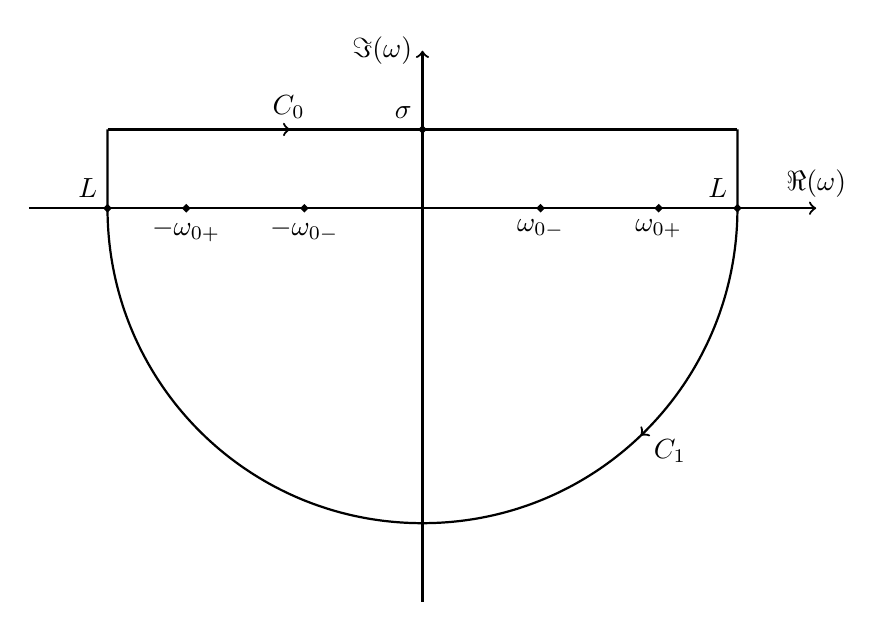
\begin{tikzpicture}[very thick,decoration={
			markings,
			mark=at position 0.29 with {\arrow{>}}}
		]
		\draw [->, thick] (-5,0) -- (5,0) node[above]{$\Re(\omega)$};
		\draw [->, thick] (0,-5) -- (0,2) node[left]{$\Im(\omega)$};
		
		\draw [postaction={decorate}, thick] (-4,1) -- (4,1);
		\draw [postaction={decorate}, thick] (4,1) to (4,0) node[above left]{$L$} to [out=-90,in=0] (0,-4) to [out=180,in=-90] (-4,0) node[above left]{$L$} to (-4,1);
		\node [above left] at (0,1) {$\sigma$};
		
		\draw[fill] (-4,0) circle [radius=0.025];
		\draw[fill] (4,0) circle [radius=0.025];
		\draw[fill] (0,1) circle [radius=0.025];
		
		\draw[fill] (3,0) circle [radius=0.025];
		\node [below] at (3,0) {$\omega_{0+}$};
		
		\draw[fill] (-3,0) circle [radius=0.025];
		\node [below] at (-3,0) {$-\omega_{0+}$};
		
		\draw[fill] (1.5,0) circle [radius=0.025];
		\node [below] at (1.5,0) {$\omega_{0-}$};
		
		\draw[fill] (-1.5,0) circle [radius=0.025];
		\node [below] at (-1.5,0) {$-\omega_{0-}$};
		
		\node [above] at (-1.7,1) {$C_0$};
		\node [below right] at (2.8,-2.8) {$C_1$};
		\end{tikzpicture} 
	}
	\caption{Bromwich contour for the complex integration of $\tilde{A}_{1,2}$.}
	\label{fig: brom cont incomp}
\end{figure}
Considering first the integral along $C_1$, the integrand in question behaves like $T_1(\omega)/kD(\omega) = \mathcal{O}(|\omega|^{-2})$, as $|\omega| \to \infty$. Therefore, the integral around the semi-circle vanishes, \textit{i.e.}
\begin{equation}
\lim_{L \to \infty} \int_{C_1} \frac{T_1(\omega)}{kD(\omega)} e^{-i\omega t} d\omega = 0.
\end{equation}

Next, since the integral along contour $C$ is integrated in the clockwise direction, it is equal to $-2\pi i$ multiplied by the sum of the residues of the poles at $\omega = \pm \omega_{0\pm}$. The residues are evaluated using L'Hopital's Rule (the requirements ensuring the validity L'Hopital's Rule in this case are verified in Appendix~\ref{app: l'hopital}). For an arbitrary choice of initial condition, $f(x,\omega)$, the residue at $\omega = \omega_{0+}$ is
\begin{align}
\mathrm{Res}&\left\{\frac{T_1(\omega)}{kD(\omega)}e^{-i\omega t}; \omega = \omega_{0+} \right\} = 
\lim_{\omega \to \omega_{0+}} \frac{(\omega - \omega_{0+})T_1(\omega)}{kD(\omega)} e^{-i\omega t} \notag \\ 
&= \lim_{\omega \to \omega_{0+}} \frac{1}{kD'(\omega)} [T_1(\omega) + (\omega - \omega_{0+})T'_1(\omega) - it(\omega - \omega_{0+})T_1(\omega)]e^{-i\omega t} \notag \\
&= \lim_{\omega \to \omega_{0+}} \frac{1}{kD'(\omega)} T_1\left[\omega \Psi_0 + i\frac{\partial \Psi_0}{\partial t}\right](\omega) e^{-i\omega t} \notag \\
&= \lim_{\omega \to \omega_{0+}} \frac{1}{kD'(\omega)} \left\{ \omega T_1[\Psi_0](\omega) + iT_1\left[\frac{\partial \Psi_0}{\partial t}\right](\omega) \right\} e^{-i\omega t} \notag \\
&= \left\{ \omega_{0+} \chi_{1+}[\Psi_0] + i\chi_{1+}\left[\frac{\partial \Psi_0}{\partial t}\right] \right\} e^{-i\omega_{0+} t},
\end{align}
where $\chi_{1+}[g] := T_1[g](\omega_{0+}) / kD'(\omega_{0+})$ is a functional mapping an arbitrary function $g$ to the real numbers. Similarly, the residues at $\omega = -\omega_{0+}$ and $\omega = \pm\omega_{0-}$ are
\begin{align}
\mathrm{Res}\left\{\frac{T_1(\omega)}{kD(\omega)}e^{-i\omega t}; \omega = -\omega_{0+} \right\} &= \left\{ \omega_{0+} \chi_{1+}[\Psi_0] - i\chi_{1+}\left[\frac{\partial \Psi_0}{\partial t}\right] \right\} e^{i\omega_{0+} t}, \\
\mathrm{Res}\left\{\frac{T_1(\omega)}{kD(\omega)}e^{-i\omega t}; \omega = \pm \omega_{0-} \right\} &= \left\{ \omega_{0-} \chi_{1-}[\Psi_0] \pm i\chi_{1-}\left[\frac{\partial \Psi_0}{\partial t}\right] \right\} e^{\mp i\omega_{0-} t},
\end{align}
respectively, where we define $\chi_{1-}[g] = T_1[g](\omega_{0-}) / kD'(\omega_{0-})$. To derive these residues, we have used the fact that $D'$ is an odd function of $\omega$, and $D$ and $T_1[g]$ are even functions of $\omega$ when the function $g$ that is constant with respect to $\omega$.

Compiling the above results, the solution of the first inverse Laplace Transform in Equation~\eqref{sol incomp} is
\begin{align}
\mathcal{L}^{-1}\left\{ \tilde{A}_1 \right\} &= \frac{1}{2\pi} \lim_{L \to \infty} \int_{C_0} \frac{T_1(\omega)}{kD(\omega)} e^{-i\omega t} d\omega \\
&= \frac{1}{2\pi} \lim_{L \to \infty} \int_{C} \frac{T_1(\omega)}{kD(\omega)} e^{-i\omega t} d\omega \notag \\
&= -i \sum \mathrm{Res}\left\{\frac{T_1(\omega)}{kD(\omega)}e^{-i\omega t}; \omega = \pm \omega_{0\pm} \right\} \notag \\
&= -i \left\{\omega_{0+}\chi_{1+}[\Psi_0] \left(e^{-i\omega_{0+} t} + e^{i\omega_{0+} t}\right) + i\chi_{1+}\left[ \frac{\partial \Psi_0}{\partial t} \right] \left(e^{-i\omega_{0+} t} - e^{i\omega_{0+} t}\right) \right. \notag \\
& \qquad\quad \left. + \omega_{0-}\chi_{1-}[\Psi_0] \left(e^{-i\omega_{0-} t} + e^{i\omega_{0-} t}\right) + i\chi_{1-}\left[ \frac{\partial \Psi_0}{\partial t} \right] \left(e^{-i\omega_{0-} t} - e^{i\omega_{0-} t}\right)\right\} \notag \\
&= -2 \left\{ i\omega_{0+}\chi_{1+}[\Psi_0] \cos(\omega_{0+} t) - \chi_{1+}\left[ \frac{\partial \Psi_0}{\partial t} \right] \sin(\omega_{0+} t) \right. \notag \\
& \qquad\quad \left. + i\omega_{0-}\chi_{1-}[\Psi_0] \cos(\omega_{0-} t) - \chi_{1-}\left[ \frac{\partial \Psi_0}{\partial t} \right] \sin(\omega_{0-} t) \right\}.
\end{align}


The second inverse Laplace transform in Equation~\eqref{sol incomp} is calculated as follows.
\begin{align}
\mathcal{L}^{-1}\left\{ \frac{\omega}{\e_1} \right\} &= \frac{1}{2\pi}\lim_{L \to \infty} \int_{i\sigma - L}^{i\sigma + L} \frac{\omega e^{-i\omega t}}{\e_1} ~d\omega \notag \\
&= \frac{1}{2\pi\rho_1}\lim_{L \to \infty} \int_{i\sigma - L}^{i\sigma + L} \frac{\omega e^{-i\omega t}}{(kv_{A1} + \omega)(kv_{A1} - \omega)} ~d\omega,
\end{align}
whose integrand has simple poles at $\omega = \pm k v_{A1}$. From Jordan's Lemma it follows that the integrand vanishes as $\omega \to \infty$. Therefore, we can construct a Bromwich contour as shown in Figure~\ref{fig: brom cont incomp 2}. The residues of the integrand at the poles are
\begin{align}
\mathrm{Res}\left\{\frac{\omega e^{-i\omega t}}{k^2v_{A1}^2 - \omega^2}; \omega = \pm kv_{A1} \right\} &= 
\lim_{\omega \to \pm kv_{A1}} \frac{(\omega \mp kv_{A1}) \omega e^{-i\omega t}}{k^2v_{A1}^2 - \omega^2} \\ 
&= -\frac{1}{2}e^{\mp ikv_{A1} t}.
\end{align}
Therefore, the second inverse Laplace transform in Equation~\eqref{sol incomp} is
\begin{equation}
\mathcal{L}^{-1}\left\{ \frac{\omega}{\e_1} \right\} = -\frac{i}{\rho_1} \sum \mathrm{Res} \left\{ \frac{\omega e^{-i\omega t}}{k^2v_{A1}^2 - \omega^2}; \omega = \pm kv_{A1} \right\} = \frac{i}{\rho_1}\cos{kv_{A1}t}.
\end{equation}

The third and final inverse Laplace transform in Equation~\eqref{sol incomp} is calculated as follows.
\begin{align}
\mathcal{L}^{-1}\left\{ \frac{1}{\e_1} \right\} &= \frac{1}{2\pi}\lim_{L \to \infty} \int_{i\sigma - L}^{i\sigma + L} \frac{e^{-i\omega t}}{\e_1} ~d\omega, \notag \\
&= \frac{1}{2\pi\rho_1}\lim_{L \to \infty} \int_{i\sigma - L}^{i\sigma + L} \frac{e^{-i\omega t}}{(kv_{A1} + \omega)(kv_{A1} - \omega)} ~d\omega,
\end{align}
whose integrand has simple poles at $\omega = \pm k v_{A1}$. Again, the integrand vanishes as $\omega \to \infty$, so we can integrate around the Bromwich contour as shown in Figure~\ref{fig: brom cont incomp 2}. The residues of the integrand at the poles are
\begin{align}
\mathrm{Res}\left\{\frac{e^{-i\omega t}}{k^2v_{A1}^2 - \omega^2}; \omega = \pm kv_{A1} \right\} &= 
\lim_{\omega \to \pm kv_{A1}} \frac{(\omega - kv_{A1}) e^{-i\omega t}}{k^2v_{A1}^2 - \omega^2} \notag \\ 
&= \mp \frac{1}{2kv_{A1}} e^{\mp ikv_{A1} t}.
\end{align}
Therefore, the final inverse Laplace transform in Equation~\eqref{sol incomp} is
\begin{align}
\mathcal{L}^{-1}\left\{ \frac{1}{\e_1} \right\} &= -\frac{i}{\rho_1} \sum \mathrm{Res} \left\{ \frac{e^{-i\omega t}}{k^2v_{A1}^2 - \omega^2}; \omega = \pm kv_{A1} \right\} \notag \\
&= \frac{1}{\rho_1kv_{A1}} \sin{kv_{A1}t}.
\end{align}

\begin{figure}
	\centering
	\scalebox{0.9}{
		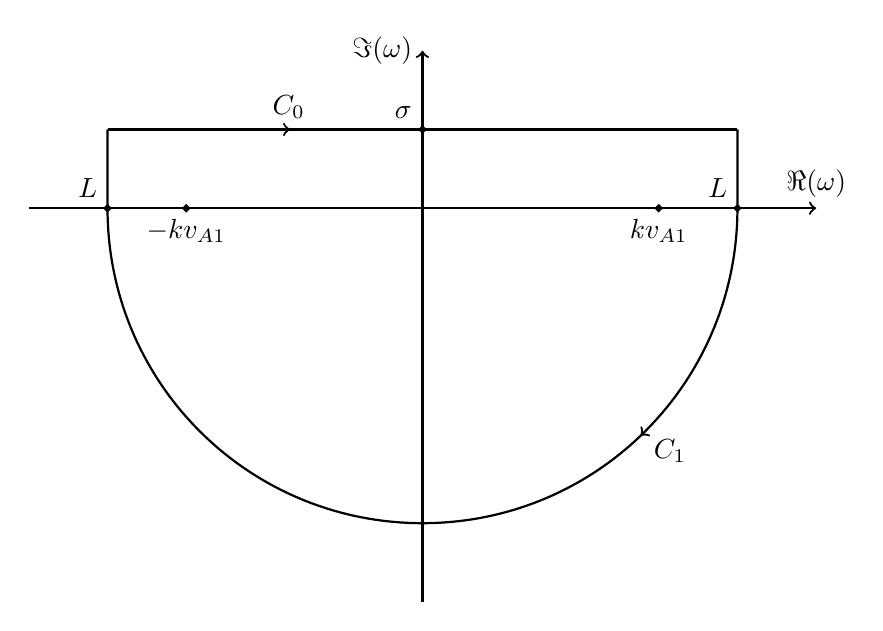
\begin{tikzpicture}[very thick,decoration={
			markings,
			mark=at position 0.29 with {\arrow{>}}}
		]
		\draw [->, thick] (-5,0) -- (5,0) node[above]{$\Re(\omega)$};
		\draw [->, thick] (0,-5) -- (0,2) node[left]{$\Im(\omega)$};
		
		\draw [postaction={decorate}, thick] (-4,1) -- (4,1);
		\draw [postaction={decorate}, thick] (4,1) to (4,0) node[above left]{$L$} to [out=-90,in=0] (0,-4) to [out=180,in=-90] (-4,0) node[above left]{$L$} to (-4,1);
		\node [above left] at (0,1) {$\sigma$};
		
		\draw[fill] (-4,0) circle [radius=0.025];
		\draw[fill] (4,0) circle [radius=0.025];
		\draw[fill] (0,1) circle [radius=0.025];
		
		\draw[fill] (3,0) circle [radius=0.025];
		\node [below] at (3,0) {$kv_{A1}$};
		
		\draw[fill] (-3,0) circle [radius=0.025];
		\node [below] at (-3,0) {$-kv_{A1}$};
		
		\node [above] at (-1.7,1) {$C_0$};
		\node [below right] at (2.8,-2.8) {$C_1$};
		\end{tikzpicture} 
	}
	\caption{Bromwich contour for the complex integration of the integrand of $J_1$.}
	\label{fig: brom cont incomp 2}
\end{figure}
Combining the above expressions for the three inverse Laplace transforms, the transverse velocity solution for $x<-x_0$ is
\begin{align}
v_x(x, t) = &-2 e^{k(x+x_0)} \left\{ i\omega_{0+}\chi_{1+}[\Psi_0] \cos(\omega_{0+} t) - \chi_{1+}\left[ \frac{\partial \Psi_0}{\partial t} \right] \sin(\omega_{0+} t) \right. \\
&\left. + i\omega_{0-}\chi_{1-}[\Psi_0] \cos(\omega_{0-} t) - \chi_{1-}\left[ \frac{\partial \Psi_0}{\partial t} \right] \sin(\omega_{0-} t) \right\} \\
&+ \frac{i}{\rho_1} \int_{-\infty}^{-x_0} G_1(x;s) \left[ \Psi(s, 0) \cos{kv_{A1}t} + \frac{\partial \Psi}{\partial t}(s, 0) \frac{\sin{kv_{A1}t}}{kv_{A_1}} \right]~ds.
\end{align}
Similarly, the transverse velocity for the region $x>x_0$ is
\begin{align}
v_x(x, t) = &-2 e^{k(x_0 - x)} \left\{ i\omega_{0+}\chi_{2+}[\Psi_0] \cos(\omega_{0+} t) - \chi_{2+}\left[ \frac{\partial \Psi_0}{\partial t} \right] \sin(\omega_{0+} t) \right. \notag \\
&\left. + i\omega_{0-}\chi_{2-}[\Psi_0] \cos(\omega_{0-} t) - \chi_{2-}\left[ \frac{\partial \Psi_0}{\partial t} \right] \sin(\omega_{0-} t) \right\} \notag \\
& + \frac{i}{\rho_2} \int_{x_0}^{\infty} G_2(x;s) \left[ \Psi(s, 0) \cos{kv_{A2}t} + \frac{\partial \Psi}{\partial t}(s, 0) \frac{\sin{kv_{A2}t}}{kv_{A_2}} \right]~ds.
\end{align}
Finally, for the region $|x| \leq x_0$, it is
\begin{align}
v_x(x, t) =& -\frac{2}{\sinh{2kx_0}} \left[ \left\{ i\omega_{0+}\chi_{1+}[\Psi_0] \cos(\omega_{0+} t) - \chi_{1+}\left[ \frac{\partial \Psi_0}{\partial t} \right] \sin(\omega_{0+} t) \right. \right. \notag \\
& \left. + i\omega_{0-}\chi_{1-}[\Psi_0] \cos(\omega_{0-} t) - \chi_{1-}\left[ \frac{\partial \Psi_0}{\partial t} \right] \sin(\omega_{0-} t) \right\} \sinh(k(x_0 - x)) \notag \\ 
& + \left\{ i\omega_{0+}\chi_{2+}[\Psi_0] \cos(\omega_{0+} t) - \chi_{2+}\left[ \frac{\partial \Psi_0}{\partial t} \right] \sin(\omega_{0+} t) \right. \notag \\
& \left. \left. + i\omega_{0-}\chi_{2-}[\Psi_0] \cos(\omega_{0-} t) - \chi_{2-}\left[ \frac{\partial \Psi_0}{\partial t} \right] \sin(\omega_{0-} t) \right\} \sinh(k(x_0 + x)) \right] \notag \\
& + \frac{i}{\rho_0} \int_{-x_0}^{x_0} G_0(x;s) \left[ \Psi(s, 0) \cos{kv_{A0}t} + \frac{\partial \Psi}{\partial t}(s, 0) \frac{\sin{kv_{A0}t}}{kv_{A0}} \right]~ds.
\end{align}

These solutions are not particularly illuminating in there general form, so we evaluate the solutions using specific initial conditions in the next subsections.


\subsubsection{Uniform initial vorticity}

Let $\Omega(x, 0) = \Omega_0$ be constant. Therefore, $\Psi_0 = k\rho_0\Omega_0$ and $\partial \Psi_0 / \partial t = 0$. To evaluate the solution, we evaluate the Green's function integral for each regions of the waveguide separately. Firstly, for $x < -x_0$, 
\begin{align}
\int_{-\infty}^{-x_0} G_1(x;s) \Psi_0 ~ds &= \Omega_0 \rho_1 \left[ \sinh(k(x+x_0)) \int_{-\infty}^{x} e^{k(s + x_0)} ~ds \right . \notag \\
&\qquad \qquad \left.+ e^{k(x+x_0)} \int_{x}^{-x_0} \sinh(k(s+x_0)) ~ds \right] \notag \\
&= \frac{\Omega_0 \rho_1}{k} \left[ e^{k(x+x_0)} - 1 \right].
\end{align}
Secondly, for $|x| \leq x_0$,
\begin{align}
\int_{-x_0}^{x_0} G_0(x;s) \Psi_0 ~ds &= \frac{\Omega_0 \rho_0}{\sinh{2kx_0}} \left[ \sinh(k(x-x_0)) \int_{-x_0}^{x} \sinh(k(s+x_0)) ~ds \right. \notag \\
&\qquad \qquad \qquad \left. + \sinh(k(x+x_0)) \int_{x}^{x_0} \sinh(k(s-x_0)) ~ds \right], \notag \\
&= \frac{\Omega_0 \rho_0}{k} \left( \frac{\cosh{kx}}{\cosh{kx_0}} - 1 \right).
\end{align}
Finally, for $x > x_0$,
\begin{align}
\int_{x_0}^{\infty} G_2(x;s) \Psi_0 ~ds &= - \Omega_0 \rho_2 \left[ e^{-k(x-x_0)} \int_{x_0}^{x} \sinh(k(s-x_0)) ~ds \right. \notag \\
&\qquad \qquad \quad \left. + \sinh(k(x-x_0)) \int_{x}^{\infty} e^{-k(s-x_0)} ~ds \right], \notag \\
&= \frac{\Omega_0 \rho_2}{k} \left[ e^{-k(x-x_0)} - 1 \right].
\end{align}
The other integrals that need to be evaluated are
\begin{align}
I_0^\pm &= \frac{\Omega_0\omega\rho_0k}{\sinh{2kx_0}} \int_{-x_0}^{x_0} \sinh(k(s \pm x_0)) ds, \\
&= \pm \frac{\Omega_0 \omega \rho_0}{\sinh{2kx_0}} (\cosh{2kx_0 - 1}),
\end{align}
\begin{align}
I_1 &= \Omega_0\omega\rho_1k \int_{-\infty}^{-x_0} e^{k(s + x_0)} ds, \\
&= \Omega_0 \omega \rho_1,
\end{align}
and
\begin{align}
I_2 &= \Omega_0\omega\rho_2k \int_{x_0}^{\infty} e^{k(x_0 - s)} ds, \\
&= \Omega_0 \omega \rho_2.
\end{align}
Using the above integrals, the transverse velocity through time for an initially constant vorticity is
\begin{equation}
v_x = -\frac{i}{k}\begin{cases}
2 e^{k(x+x_0)} A^*_1 + \Omega_0 \left\{1 - e^{k(x+x_0)}\right\} \cos{kv_{A1}t} \quad &\text{ for } x<-x_0, \\
\frac{2}{\sinh{2kx_0}} \left[ A^*_1 \sinh(k(x_0 - x)) + A^*_2 \sinh(k(x_0 + x)) \right] & \\
+ \Omega_0 \left( 1 - \frac{\cosh{kx}}{\cosh{kx_0}} \right)\cos{kv_{A0}t} \quad &\text{ for } x < |x_0|, \\
2 e^{k(x_0-x)} A^*_2 + \Omega_0 \left\{1 - e^{k(x_0-x)}\right\} \cos{kv_{A2}t} \quad &\text{ for } x>x_0, \\
\end{cases}
\label{sol slab}
\end{equation}
where
\begin{equation}
A^*_{1,2} = \omega_{0+} \frac{T_{1,2}[\psi_0](\omega_{0+})}{D'(\omega_{0+})} \cos(\omega_{0+} t) + \omega_{0-}\frac{T_{1,2}[\psi_0](\omega_{0-})}{D'(\omega_{0-})} \cos(\omega_{0-} t),
\end{equation}
and
\begin{align}
T_{1,2}[\Psi_0](\omega) = &-\Omega_0\{ (\rho_0 \tanh(kx_0) + \rho_{1,2}) (\e_0 \cosh(2kx_0) + \e_{2,1}\sinh(2kx_0)) \notag \\
&+ \e_0(\rho_0 \tanh(kx_0) + \rho_{2,1}) \}.
\end{align}

When $\rho_1 = \rho_2 = \rho_0$ and $x_0 = 0$, the solution given by Equation~\eqref{sol slab} reduces with that of a tangential interface, Equation~\eqref{sol int}.

The time-dependant evolution of a perturbation of an incompressible asymmetric magnetic slab are thus purely superposition of normal modes. There is no contribution from the continuous spectrum. There is instantaneous set-up of coherently oscillating collective modes. It is the introduction of compressibility that introduces a continuous spectrum, and therefore a leaky component to the oscillation. This is the subject of the following subsection.


\subsection{Compressible slab} \label{sec: compressible slab}

In this subsection, we solve the initial value problem of a compressible asymmetric slab. 

The more general compressible version of Equation~ \eqref{gov reduced} is
\begin{equation}
\tilde{v}_x'' - m^2 \tilde{v}_x = g(x, \omega),
\end{equation}
where
\begin{equation}
g(x, \omega) = \frac{1}{(c_0^2 + v_A^2)(\omega_T^2 - \omega^2)}\left[ (\omega_0^2 - \omega^2)\left(\dot{\widehat{v}}_{x0} - i\omega \widehat{v}_{x0}\right) + ikc_0^2\left( \dot{\widehat{v}}_{z0}' - i\omega \widehat{v}_{z0}'\right) \right]. \label{ODE compressible}
\end{equation}
This equation can be reduced to the corresponding equation for incompressible plasma in the limit of infinite sound speed, \textit{i.e.} $c_0 \to \infty$.
Equation~\eqref{ODE compressible} corroborates with the general initial value problem considered by \cite{and_etal07}, although some algebra is required to transform between velocity and total pressure coordinates.

Considering a magnetic slab in a non-magnetic environment, we have
\begin{align}
m_0^2 &= \frac{(\omega_0^2 - \omega^2)(\omega_A^2 - \omega^2)}{(c_0^2 + v_A^2)(\omega_T^2 - \omega^2)}, \quad m_{1,2}^2 = \frac{\omega_{1,2}^2 - \omega^2}{c_{1,2}^2}, \\
g_{1,2}(x, \omega) &= \frac{1}{c_0^2\omega^2} \left[ (\omega_0^2 - \omega^2)\left(\dot{\widehat{v}}_{x0} - i\omega \widehat{v}_{x0}\right) + ikc_0^2\left( \dot{\widehat{v}}_{z0}' - i\omega \widehat{v}_{z0}'\right) \right].
\end{align}


\subsubsection{Solution in Laplace space}

For the solution inside the slab, $|x| \leq x_0$, $\widehat{v}_x(x)$ satisfies
\begin{equation}
\left( \frac{\partial^2}{\partial x^2} - m_0^2 \right) \tilde{v}_x = g_0(\omega, x), \label{vx eq inside}
\end{equation}
under the boundary conditions $\tilde{v}_x(-x_0) = \tilde{A}_1$ and $\tilde{v}_x(-x_0) = \tilde{A}_2$. To solve this we construct the Green's function, $G_0(x;s)$ that satisfies
\begin{equation}
\frac{d^2G_0}{dx^2} - m_0^2 G_0 = \delta(x-s), \quad G_0(-x_0;s) = G_0(x_0;s) = 0.
\end{equation}
The general solution of this equation is
\begin{equation}
G_0(x;s) = c_1\sinh(m_0(x - x_0)) + c_2\sinh(m_0(x + x_0)),
\end{equation}
where $c_1 = 0$ for $x < s$ and $c_2 = 0$ for $x > s$. Ensuring $G_0$ and $\partial G_0 / \partial x$ have jumps of 0 and 1 at $x = s$, respectively, determines $c_1$ and $c_2$ so that $G_0(x;s)$ is
\begin{equation}
G_0(x;s) = \frac{-1}{m_0\sinh(2m_0 x_0)}
\begin{cases}
\sinh(m_0(x_0 - s))\sinh(m_0(x_0 + x)), & \text{if } -x_0<x<s, \\
\sinh(m_0(x_0 - x))\sinh(m_0(x_0 + s)), & \text{if } s<x<x_0.
\end{cases}
\end{equation}
Then the solution of Equation~\eqref{vx eq inside} is
\begin{align}
\tilde{v}_x(x) = &\frac{1}{m_0\sinh{2m_0 x_0}} \left[ \tilde{A}_1\sinh(m_0(x_0 - x)) + \tilde{A}_2\sinh(m_0(x_0 + x)) \right] \notag \\
&+ \int_{-x_0}^{x_0} G_0(x;s) g_0(\omega, s) ~ds.
\label{V sol 0}
\end{align}
This is the sum of the Green's function term and a two terms that are independent solutions to the homogeneous version of Equation~\eqref{vx eq inside} that ensure that the inhomogeneous boundary conditions are satisfied.

For the solution outside and to the left of the slab, $x < -x_0$, $\tilde{v}_x(x)$ satisfies
\begin{equation}
\left(\frac{d^2}{dx^2} - m_1^2 \right) \tilde{v}_x = g_1(\omega, x),
\end{equation}
and the boundary conditions $\tilde{v}_x(-\infty) = 0$, $\tilde{v}_x(-x_0) = \tilde{A}_1$. By following a Green's function method, the solution of this Sturm-Liouville system is
\begin{equation}
\tilde{v}_x(x) = \tilde{A}_1e^{m_1(x_0+x)} + \int_{-\infty}^{-x_0} G_1(x; s) g_1(\omega, s) ds,
\label{V sol 1}
\end{equation}
where $m_1 > 0$ and the Green's function, $G_1$, is defined by
\begin{equation}
G_1(x; s) = \frac{1}{m_1}
\begin{cases}
e^{m_1(x_0 + x)}\sinh(m_1(x_0 + s)), & \text{if } x < s, \\
e^{m_1(x_0 + s)}\sinh(m_1(x_0 + x)), & \text{if } s < x < -x_0.
\end{cases}
\end{equation}

Similarly, the solution outside and to the right of the slab, $x > x_0$, is
\begin{equation}
\tilde{v}_x(x) = \tilde{A}_2e^{m_2(x_0-x)} + \int_{x_0}^{\infty} G_2(x; s) g_2(\omega, s) ~ds,
\label{P sol 2}
\end{equation}
where $m_2 > 0$ and the Green's function, $G_2$, is defined by
\begin{equation}
G_2(x; s) = \frac{1}{m_2}
\begin{cases}
e^{m_2(x_0 - s)}\sinh(m_2(x_0 - x)), & \text{if } x_0 < x < s, \\
e^{m_2(x_0 - x)}\sinh(m_2(x_0 - s)), & \text{if } s < x.
\end{cases}
\end{equation}

Putting all of this together, the Laplace transform of the transverse velocity is
\begin{equation}
\tilde{v}_x(x) = 
\begin{cases}
\tilde{A}_1e^{m_1(x_0 + x)} + \int_{-\infty}^{-x_0} G_1(x; s) g_1(\omega, s) ~ds, & \text{if } -\infty < x < -x_0, \\

\frac{1}{\sinh{2m_0x_0}} \left[ \tilde{A}_1\sinh(m_0(x_0 - x)) + \tilde{A}_2\sinh(m_0(x_0 + x)) \right]  \\
+ \int_{-x_0}^{x_0} G_0(x; s) g_0(\omega, s) ~ds, & \text{if } |x| \leq x_0, \\

\tilde{A}_2e^{m_2(x_0 - x)} + \int_{x_0}^{\infty} G_2(x; s) g_2(\omega, s) ~ds, & \text{if } x_0 < x < \infty.
\end{cases}
\label{V sol}
\end{equation}


\subsubsection{Matching solutions}

For physically relevant solutions, we require that the transverse velocity and the total pressure be continuous across the interfaces at $x = \pm x_0$.

Continuity in transverse velocity, $\tilde{v}_x$, is satisfied automatically by considering the solutions inside and outside the slab given by Equations~\eqref{V sol}, and our definition of $\tilde{A}_1 = \tilde{v}_x(-x_0)$ and $\tilde{A}_2 = \tilde{v}_x(x_0)$.

Continuity in total pressure can be dealt with as follows. The perturbation in total pressure is related to the velocity gradient by\footnote{Found by combining that induction equation with the momentum equation, see, for example, the bottom row of Equation~(2) by \cite{and_etal07}.}
\begin{equation}
\frac{\partial p_T}{\partial t} = -\rho\left[ \left(c_0^2 + v_A^2\right) \frac{\partial v_x}{\partial x} + c_0^2\frac{\partial v_z}{\partial z} \right].
\end{equation}
Looking for solutions proportional to $\exp{ikz}$ and taking Laplace transforms in time leads to
\begin{equation}
\tilde{p}_T = -\frac{i\rho}{\omega} \frac{(c_0^2 + v_A^2)(\omega_T^2 - \omega^2)}{(\omega_0^2 - \omega^2)} \tilde{v}_x' + \frac{i}{\omega} \widehat{p}_{T0} + \frac{\rho \omega^2}{k\omega(\omega_0^2 - \omega^2)} \left(\dot{\widehat{v}}_{z0} - i\omega\widehat{v}_{z0}\right).
\end{equation}
Therefore, if we make the simplification\footnote{This simplification is not as strict as it might first seem. For example, any pressure perturbation-free transverse kick, such as you might expect from a nearby flare, would do.} to the prescribed initial conditions such that
\begin{equation}
\widehat{p}_{T0} - \frac{\rho \omega_0^2}{k(\omega_0^2 - \omega^2)} \left(i\widehat{v}_{z0} + \omega\dot{\widehat{v}}_{z0}\right) = 0,
\end{equation}
then the continuity in total pressure boundary condition is equivalent to
\begin{equation}
\left[ \left[ \frac{\Lambda}{m} \frac{\partial \tilde{v}_x}{\partial x} \right] \right]_{x=\pm x_0} = 0,
\end{equation}
where double brackets indicate a jump in the quantity,
\begin{equation}
[[f]]_{x=x_0} = \lim_{\epsilon \to 0} [f(x_0 + \epsilon) - f(x_0 - \epsilon)].
\end{equation}

Substituting the solutions given by Equation~\eqref{V sol} into these boundary conditions gives
\begin{equation}
\tilde{A}_1(\omega) = \frac{T_1(\omega)}{D(\omega)}, \quad \tilde{A}_2(\omega) = \frac{T_2(\omega)}{D(\omega)},
\end{equation}
where
\begin{align}
T_1(\omega) = T_1[f](\omega) = & -(\Lambda_0\cosh{2m_0 x_0} + \Lambda_2\sinh{2m_0 x_0})(\Lambda_0 I_0^- + \Lambda_1 I_1) \notag \\
& - \Lambda_0(\Lambda_0 I_0^+ + \Lambda_2 I_2), \\
T_2(\omega) = T_2[f](\omega) = & - (\Lambda_0\cosh{2m_0 x_0} + \Lambda_1\sinh{2m_0 x_0})(\Lambda_0 I_0^+ + \Lambda_2 I_2) \notag \\
& -\Lambda_0(\Lambda_0 I_0^- + \Lambda_1 I_1), \\
D(\omega) = & \Lambda_0(\Lambda_1 + \Lambda_2)\cosh(2m_0x_0) + (\Lambda_0^2 + \Lambda_1\Lambda_2)\sinh(2m_0x_0),
\label{D}
\end{align}
where $\Lambda_j = \rho_j (\omega^2 - \omega_{Aj}^2) /  m_j$, for $j = 0, 1, 2$, and
\begin{align}
I_0^\pm &= I_0^\pm[f] = \frac{1}{m_0} \int_{-x_0}^{x_0} \frac{\sinh(m_0(x_0 \pm s))}{\sinh(2m_0x_0)} f(\omega, s) ~ds, \\
I_1 &= I_1[f] = \frac{1}{m_1} \int_{-\infty}^{-x_0} e^{m_1(s + x_0)} f(\omega, s) ~ds, \\
I_2 &= I_2[f] = \frac{1}{m_2} \int_{x_0}^\infty e^{m_2(x_0 - s)} f(\omega, s) ~ds.
\end{align}


\subsubsection{Solution in time}

To recover the transverse velocity, $v_x(x, t)$, we employ the inverse Laplace transform (non-standard, discussed in Appendix~\ref{app: laplace trans}), such that
\begin{equation}
\widehat{v}_x(x,t) = \mathcal{L}^{-1}\{\tilde{v}_x(x)\} = \frac{1}{2\pi} \lim_{L \to \infty} \int_{i\sigma - L}^{i\sigma + L} \tilde{v}_x(x) e^{-i\omega t} d\omega,
\label{laplace transform}
\end{equation}
where $\sigma$ is a real number such that all the singularities of the integrand are below the contour of integration to ensure that all singularities contribute to the integral. The integral is evaluated along an infinite horizontal line in the upper half of the complex plane and is dependent on the singularities (with respect to $\omega$) of $\tilde{v}_x$, whose residues determine the value of the contour integral. Focusing firstly on the region $x < -x_0$, the solution is
\begin{align}
\widehat{v}_x(x, t) &= \mathcal{L}^{-1} \left\{ \tilde{A}_1 e^{m_1(x + x_0)} + \int_{-\infty}^{-x_0} G_1(x; s)f_1(\omega, s)ds \right\}, \\
&= \mathcal{L}^{-1} \left\{ \tilde{A}_1 e^{m_1(x + x_0)} \right\} + \mathcal{L}^{-1} \left\{ \int_{-\infty}^{-x_0} G_1(x; s)f_1(\omega, s)ds \right\}.
\label{vx sol inv LPT}
\end{align}

To study the time-dependent behaviour of the transverse velocity, we start by studying the asymptotic behaviour of
\begin{equation}
A_1(t) = v_x(-x_0, t) = \frac{1}{2\pi} \lim_{L \to \infty} \int_{i\sigma - L}^{i\sigma + L} \frac{T_1(\omega)}{D(\omega)} e^{-i\omega t} d\omega.
\label{A inv laplace}
\end{equation}
Since the problem of finding the solution is now reduced to solving a complex integral, it is dependent on the singularities (with respect to $\omega$) of $T_1$, $T_2$, and $D$ and the zeros of $D$. Identifying the singularities allows us to modify the contour so that it is confined to a single-valued branch and the zeroes of $D$ are poles of the integrand whose residues determine the value of the modified contour integral.

To determine the singularities of  $T_1$, $T_2$, and $D$, we determine the singularities of the constituent functions, as follows:
\begin{itemize}
	\item The functions $\Lambda_j^2$ are rational functions of $\omega$ with simple poles at $\omega = \pm \omega_{0j}$, for $j = 0, 1, 2$.
	
	\item $\Lambda_j$, for $j = 0, 1, 2$, involve radicals and have branch points at $\omega = \pm \omega_{Aj}$, $\pm \omega_{0j}$, and $\pm \omega_{Tj}$, respectively.\footnote{More precisely, $\omega = \pm \omega_{Aj}$, $\pm \omega_{0j}$, and $\pm \omega_{Tj}$ are the ramification points corresponding to the branch points $\Lambda_j(\omega)$, each with ramification index 2. However, the language used in the main text is common shorthand that is considered synonymous.}
	
	\item The functions $\cosh{z}$ and $\sinh{z}$ are entire functions of $z$ with only even and odd terms in their respective series expansions. Therefore, $\cosh{z}$ and $z\sinh{z}$ are entire functions of $z^2$. Hence, $\cosh{2m_0x_0}$ and $\Lambda_0\sinh{2m_0x_0}$ have only simple poles at $\omega = \pm\omega_{T0}$.
	
	\item The integrands of $I_0^\pm$ are integrated with respect to $s$. Therefore, the singularities of $I_{1,2}$ are precisely the singularities of the integrands. The function $g(z) = \sinh(az) / \sinh(bz)$, for constants $a$ and $b \neq 0$ are entire functions of $z$, containing only even powers (once $g$ has been redefined as to remove the removable singularity at $z = 0$). Therefore, for another complex function $h$, the singularities of the composition $g \cdot h$ are precisely the singularities of the function $h(z^2)$. Hence, by letting $h(\omega) = m_0$, $a = s \pm x_0$, and $b = 2x_0$, it follows that $\sinh(m_0(s - x_0)) / \sinh(2m_0x_0)$ has simple poles at $\omega = \pm \omega_{T0}$.
	
	\item To determine the singularities of $I_{1,2}$, we need consider the singularities of the integrands. The functions $e^{\pm a\sqrt{z}}$, for constant $a \neq 0$ have branch points at $z = 0$ that are algebraic (of ramification index 2). Therefore, by setting $a = x_0 \pm s$, it follows that the functions $e^{m_j(x_0 \pm s)}$, and therefore $I_j$, have algebraic branch points at $\omega = \pm \omega_{Aj}$, $\pm \omega_{0j}$, and $\pm \omega_{Tj}$.
\end{itemize}
The set of branch points of a sum of functions is the union of the branch points of the constituent functions. Therefore, the branch points of both $T_1$, $T_2$, and $D$ are $\omega = \pm \omega_{A0,1,2}$, $\pm \omega_{00,1,2}$, $\pm \omega_{T0,1,2}$.

$T_1$ and $T_2$ have no other singularities. Therefore, the poles of $\tilde{A}_1$ and $\tilde{A}_2$ are precisely the zeroes of the dispersion function $D$. The subset of these zeroes that are real are the eigenfrequencies of the asymmetric slab studied in Chapter~\ref{chap: EVP} and the subset that are complex are the leaky modes. There is a rich spectrum of eigenmodes which,in the absence of any simplification to the model, are not possible to describe analytically.

The integrand has 18 branch points and an infinite number of poles that are not possible to describe analytically. This is a very difficult problem to solve analytically. Therefore, we will instead solve the simplified problem of a thin symmetric slab with zero-beta plasma. From there, we will study what would happen when symmetry is broken (Section~\ref{sec: generalising to asym slab}).

\subsubsection{Solving a simplified case - thin zero-beta symmetric slab}

When simplifying to a symmetric slab, we use the notation subscript $e$ to denote the symmetric \textit{external} environment, rather than subscripts 1 and 2. Now that we are considering a symmetric slab, the parameters on each side of the slab are equal. Under the zero-beta approximation, the tube speed is identical to the sound speed. Therefore, the branch points at $\omega = \pm \omega_{00,e}$ and $\omega = \pm\omega_{T0,e}$ degenerate. The remaining branch points are $\omega = \pm \omega_{A0,e}$.

Under the zero-beta approximation, the dispersion relation for a symmetric slab simplifies to
\begin{equation}
\rho_ev_{Ae}^2m_e\left(
\begin{matrix}
\tan \\
-\cot
\end{matrix} \right)(n_0x_0) = -\rho_0v_{A0}^2n_0,
\end{equation}
where $n_0^2 = -m_0^2 \approx \omega^2/v_{A0}^2 - k^2$ and $m_e^2 \approx k^2 - \omega^2/v_{Ae}^2$. \cite{edw_etal82} noticed that this is precisely the dispersion relation for Love waves, which are horizontally polarized surface wave that appears in Earth seismology \citep{lov11}. Equilibrium pressure balance requires that $\rho_ev_{Ae}^2 = \rho_0v_{A0}^2$, therefore, the dispersion relation reduces to
\begin{equation}
\left(
\begin{matrix}
\tan \\
-\cot
\end{matrix} \right)(n_0x_0) = -\frac{n_0}{m_e}.
\end{equation}
The $\tan$ version of this equation describes sausage modes and the $\cot$ version describes kink modes.

With the aim of finding solutions to this dispersion relation, we start with the equation describing kink modes. By letting the non-dimensional slab width, $kx_0$, be small, we can expand the eigenfrequencies of the first-order kink body mode as a polynomial in $kx_0$, the largest two terms of which are
\begin{equation}
\omega = \pm kv_{Ae}\left[ 1 - \frac{1}{2}\left( \frac{v_{Ae}^2}{v_{A0}^2} - 1 \right) (kx_0)^2 \right].
\end{equation}
This is the only eigenmode of the low-beta slab. It is equivalent to the fast principal kink mode in a magnetic flux tube described by \cite{cal03}. For this reason, we refer to this mode as the fast principal kink mode of a magnetic slab. The other zeros have non-zero imaginary part and therefore have a decreasing amplitude over time. They are leaky modes. To find these, we must first investigate on which Riemann sheet we expect them to be. In this case, the branch points are due to the square root functions in $m_e$ and $n_0$. These functions are double-valued so each contribute two branches. The branches of the function $m_e$ determine the behaviour of the velocity outside the slab. Outside the slab, the transverse velocity has the form $\tilde{v}_x = \tilde{A}_1e^{m_e(x_0 + x)}$ plus terms due to the inverse Laplace transform of the Green's function term (Equation~\ref{V sol}). Trapped modes require that $v_x \to 0$ as $x \to \infty$. This is only possible when $\mathrm{Re}\{m_e\} > 0$, which for trapped modes simplifies to $m_e > 0$. For the trapped mode, we have $\omega < \omega_{Ae}$, therefore to ensure that $m_e > 0$, we must take the positive square root in the definition of $m_e$. This ensures that the trapped modes are physical, by which we mean that they do not perturb plasma far from the slab. Therefore, we define the positive branch of $m_e$ as the \textit{principle sheet}\footnote{Due to it's physically relevant solutions, the equivalent of this sheet in the cylindrical problem has been labelled as the \textit{physical sheet} \citep{rud_etal06b}.}.

On the other hand, for leaky modes, we require that $v_x \nrightarrow 0$ as $x \to \infty$. Therefore, these modes must exist on the Riemann sheet defined by the negative square root in $m_e$. This is the \textit{non-principle sheet}\footnote{Also known as the \textit{non-physical sheet} \citep{rud_etal06b}}.

Leaky kink modes on the non-principle sheet are complex solutions to the equation
\begin{equation}
\tan\left(kx_0\sqrt{\frac{\omega^2}{\omega_0^2} - 1}\right) = -\frac{\sqrt{1 - \frac{\omega^2}{\omega_e^2}}}{\sqrt{\frac{\omega^2}{\omega_0^2} - 1}}.
\end{equation}
This equation admits solutions where the argument of the $\tan$ function remains finite as $kx_0 \to \infty$. For this to be satisfied, the solution must be of the form $\omega = \nu / kx_0$, where $\nu$ is independent of $kx_0$. Substituting this ansatz into the above equation and using the fact that $\tan$ is $\pi$-periodic, we find that the leaky kink mode solutions, for small $kx_0$, are
\begin{equation}
\omega = \frac{v_{A0}}{x_0}\left[ n\pi - i\tanh^{-1}\left( \frac{v_{A0}}{v_{Ae}} \right) \right],
\end{equation}
for $n \in \mathbb{Z}$.

Similarly, the leaky sausage modes on the non-principle sheet are complex solutions to the equation
\begin{equation}
\tan\left(kx_0\sqrt{\frac{\omega^2}{\omega_0^2} - 1}\right) = \frac{\sqrt{\frac{\omega^2}{\omega_0^2} - 1}}{\sqrt{1 - \frac{\omega^2}{\omega_e^2}}}
\end{equation}
and are given by
\begin{equation}
\omega = \frac{v_{A0}}{x_0}\left[ (n + \frac{1}{2})\pi - i\tanh^{-1}\left( \frac{v_{A0}}{v_{Ae}} \right) \right],
\end{equation}
for small $kx_0$ and for $n \in \mathbb{Z}$. It is easy to see that, for each pole, one can construct an open ball centred on the pole that contains no other poles, therefore all the poles are isolated. These sausage and kink leaky modes are the slab versions of the ``leaky trig mode" defined in a magnetic flux tube by \cite{cal03}.

The integrals in question given in Equation~\eqref{A inv laplace} can be calculated using the Bromwich contour in Figure~\ref{fig: brom contour}. To ensure that the contour remains on a single Riemann surface, it is modified around the branch cuts so as to encircle the poles. The closed contour $C$ is a sum of the following sub-contours:
\begin{itemize}
	\item $C_0$: the horizontal line with imaginary part $\sigma$.
	\item $C_1$: the horizontal line from $L + \delta i$ to $\omega_{Ae} + \delta i$, round the semicircle of radius $\delta$ and back along the horizontal line from $\omega_{Ae} - \delta i$ to $L - \delta i$.
	\item $C_2$: the vertical lines from $\pm L + \sigma i$ to $\pm L + \delta i$ and the arcs of the large semicircle centred at the origin with radius $L$.
	\item $C_3$: the vertical line up to, around, and back down from $\omega_{A0}$.
	\item $C_4$: the vertical line up to, around, and back down from $-\omega_{A0}$.
	\item $C_5$: the horizontal line from $-L - \delta i$ to $-\omega_{Ae} - \delta i$, round the semicircle of radius $\delta$ and back along the horizontal line from $-\omega_{Ae} + \delta i$ to $-L + \delta i$.
\end{itemize}
The integral in the inverse Laplace transform along the horizontal line is the same as the integral along the closed contour minus the integrals along the other constituent contours, \textit{i.e.} $C_0 = C - \sum_{n = 1}^{5}C_n$. The integrals along each of the contours $C$ and $C_1$ to $C_5$ are calculated in the following subsections.

\begin{figure}
	\centering
	\scalebox{0.9}{
		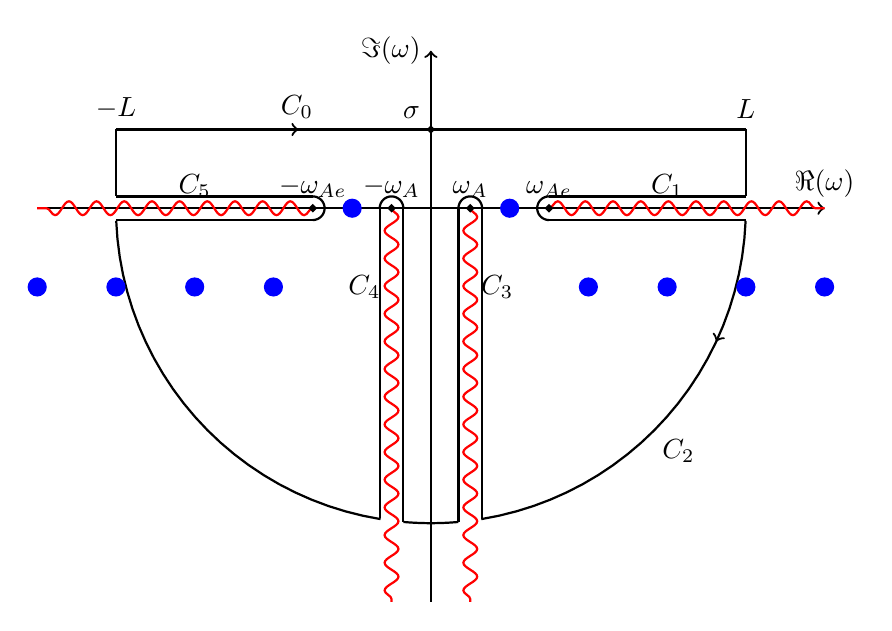
\begin{tikzpicture}[very thick, decoration={
			markings,
			mark=at position 0.29 with {\arrow{>}}}
		]
		
		\tikzset{
			branchcut/.style={decorate, decoration={snake}, draw=red}, 
		}
		
		\draw [->, thick] (-5,0) -- (5,0) node[above]{$\Re(\omega)$};
		\draw [->, thick] (0,-5) -- (0,2) node[left]{$\Im(\omega)$};
		
		\draw [postaction={decorate}, thick] (-4,1) -- (4,1);
		\draw [thick] (-4,1) -- (-4,0.15);
		\draw [thick] (4,1) -- (4,0.15);
		\draw [thick] (-4,0.15) -- (-1.5,0.15);
		\draw [thick] (4,0.15) -- (1.5,0.15);
		\draw [thick] (-4,-0.15) -- (-1.5,-0.15);
		\draw [thick] (4,-0.15) -- (1.5,-0.15);
		
		\draw [branchcut, thick] (0.5, 0) -- (0.5, -5);
		\draw [branchcut, thick] (-0.5, 0) -- (-0.5, -5);
		\draw [branchcut, thick] (1.5, 0) -- (5, 0);
		\draw [branchcut, thick] (-1.5, 0) -- (-5, 0);
		
		\draw [thick,domain=90:-90] plot ({0.15*cos(\x) - 1.5}, {0.15*sin(\x)});
		\draw [thick,domain=90:270] plot ({0.15*cos(\x) + 1.5}, {0.15*sin(\x)});
		
		\draw [postaction={decorate}, thick,domain=-2.3:-80.8] plot ({4*cos(\x)}, {4*sin(\x)});
		\draw [thick,domain=-85:-95] plot ({4*cos(\x)}, {4*sin(\x)});
		\draw [thick,domain=182.3:260.8] plot ({4*cos(\x)}, {4*sin(\x)});
		
		\draw [thick] (-0.35,0) -- (-0.35,-3.99);
		\draw [thick] (0.35,0) -- (0.35,-3.99);
		
		\draw [thick] (-0.65,0) -- (-0.65,-3.94);
		\draw [thick] (0.65,0) -- (0.65,-3.94);
		
		\draw [thick,domain=180:0] plot ({0.15*cos(\x) - 0.5}, {0.15*sin(\x)});
		\draw [thick,domain=180:0] plot ({0.15*cos(\x) + 0.5}, {0.15*sin(\x)});
		
		\node [above left] at (0,1) {$\sigma$};
		
		\draw[fill] (0,1) circle [radius=0.025];
		
		\draw[fill] (1.5,0) circle [radius=0.025];
		\node [above] at (1.5,0) {$\omega_{Ae}$};
		
		\draw[fill] (-1.5,0) circle [radius=0.025];
		\node [above] at (-1.5,0) {$-\omega_{Ae}$};
		
		\draw[fill] (0.5,0) circle [radius=0.025];
		\node [above] at (0.5,0) {$\omega_{A}$};
		
		\draw[fill] (-0.5,0) circle [radius=0.025];
		\node [above] at (-0.5,0) {$-\omega_{A}$};
		
		\draw[fill, blue] (-1,0) circle [radius=0.1];
		
		\draw[fill, blue] (1,0) circle [radius=0.1];
		
		\draw[fill, blue] (-2,-1) circle [radius=0.1];
		
		\draw[fill, blue] (-3,-1) circle [radius=0.1];
		
		\draw[fill, blue] (-4,-1) circle [radius=0.1];
		
		\draw[fill, blue] (-5,-1) circle [radius=0.1];
		
		\draw[fill, blue] (2,-1) circle [radius=0.1];

		\draw[fill, blue] (3,-1) circle [radius=0.1];
		
		\draw[fill, blue] (4,-1) circle [radius=0.1];
		
		\draw[fill, blue] (5,-1) circle [radius=0.1];
		
		\node [above] at (-1.7,1) {$C_0$};
		\node [above] at (3,0) {$C_1$};
		\node [below right] at (2.8,-2.8) {$C_2$};
		
		\node [right] at (0.5,-1) {$C_3$};
		\node [left] at (-0.5,-1) {$C_4$};
		\node [above] at (-3,0) {$C_5$};
		
		\node [above] at (4,1) {$L$};
		\node [above] at (-4,1) {$-L$};
		\end{tikzpicture} 
	}
	\caption{The Bromwich contour, $C = \sum_{n = 0}^{5}C_n$, for the complex integration of $\tilde{A}_{1,2}$ in the inverse Laplace transform in Equation~\eqref{A inv laplace}. The radius of the large semicircle is $L$ and the radius of the small semicircles around the points $\pm \omega_0$ and $\pm \omega_T$ is $\delta$. The blue circles are the poles and the red lines indicate the branch cuts.}
	\label{fig: brom contour}
\end{figure}

\subsubsection{Integral along $C$}
The contour $C$ is closed and has been chosen such that the integrand can be made to be meromorphic on this contour, given a particular choice of Riemann sheet. Therefore, we would like to use the Residue Theorem to calculate this integral. While the Residue Theorem is often quoted with a restriction to a finite number of isolated poles, it is also valid when there are infinitely many isolated poles \citep{ahl79}.

The residue of the principal kink mode is calculated as follows. First, we must determine the order of the pole. The order of the pole is equivalent to the order of the corresponding zero of the dispersion function. The dispersion function for a symmetric slab can be factorised into a product of a functions governing sausage and kink modes, namely
\begin{equation}
D(\omega) = -2\rho_0^2v_{A0}^4 \frac{\cosh{2m_0x_0}}{\tanh{m_0x_0} + \coth{m_0x_0}} D_s(\omega) D_k(\omega),
\end{equation}
where
\begin{equation}
D_s(\omega) = m_0 + m_e\tanh{m_0x_0} \quad \text{and} \quad D_k(\omega) = m_0 + m_e\coth{m_0x_0}.
\end{equation}
Denote the principal kink eigenfrequency by $\omega_k$. We know that $D_s(\omega_k) \neq 0$. We can expand the function $D_k$ as a Taylor series about the frequency $\omega_k$ as
\begin{equation}
D_k(\omega) = D_k(\omega_k) + D_k'(\omega)(\omega - \omega_k) + O((\omega - \omega_k)^2).
\end{equation}
Then, the order of $\omega_k$ as a zero of $D_k$ (and hence of $D$) is determined by the order of the first derivative of $D_k$ that is not small when evaluated at $\omega_k$. First, we check the order of $D_k'(\omega_k)$. Using the product and chain rules,
\begin{equation}
D_k'(\omega) = \omega\left[ \frac{1}{v_{A0}^2m_0} (m_e\text{csch}^2{m_0x_0} - 1) - \frac{1}{v_{Ae}^2m_e}\coth{m_0x_0} \right].
\end{equation}
Evaluated at $\omega = \omega_k$, it can easily be shown that $D_k'(\omega_k) = O(1)$ with respect to the small quantity $kx_0$. In particular, $D_k'(\omega_k)$ is not small. Therefore, $\omega_k$ is a simple pole of the integrand.

The residues of the forwards and backwards propagating principal kink modes are thus
\begin{align}
\text{Res}&\left\{ \frac{T_1}{D} e^{-i\omega t} ; \omega = \omega_k \right\} = \lim_{\omega \to \omega_k} (\omega - \omega_k)\frac{T_1(\omega)}{D(\omega)} e^{-i\omega t} \notag \\
&= \lim_{\omega \to \omega_k}\frac{1}{D'(\omega)} [T_1(\omega) + (\omega - \omega_k)T_1'(\omega) - it(\omega - \omega_k)T_1(\omega)]e^{-i\omega t} \notag \\
&= \lim_{\omega \to \omega_k} \frac{T_1(\omega)}{D'(\omega)}e^{-i\omega t} \notag \\
&= \chi_1^{(k)} e^{-i\omega_k t},
\end{align}
where $\chi_1^{(k)} = T_1(\omega_k)/D(\omega_k)$. L'Hopital's rule was used in the above derivation. Similarly, 
\begin{equation}
\text{Res}\left\{ \frac{T_1}{D} e^{-i\omega t} ; \omega = -\omega_k \right\} = -\chi_1^{(k)} e^{i\omega_k t},
\end{equation}
because $T_1$ is an even functions of $\omega$ and $D'$ is an odd function of $\omega$. The sum of these two residues is
\begin{equation}
-2i\chi_1^{(k)}\sin{\omega_k t}.
\end{equation}

The residues at the leaky kink modes can be calculated as follows. We denote the eigenfrequency of the $n$th leaky kink mode as $\omega_{kn}$. Following the same line of reasoning as for the principal kink mode, $D'(\omega_{kn}) = O(1)$ with respect to $kx_0$, so $D'(\omega_{kn})$ is not small. Therefore, these poles are simple. The residue at $\omega_{kn}$, for $n \in \mathbb{Z}$, is
\begin{equation}
\text{Res}\left\{ \frac{T_1}{D} e^{-i\omega t} ; \omega = \omega_{kn} \right\} = \chi_1^{(kn)} e^{-i\omega_{kn} t},
\end{equation}
where $\chi_1^{(kn)} = T_1(\omega_{kn})/D(\omega_{kn})$. Since, $\omega_{kn}$ is complex, it is instructive to split it up into its real and imaginary parts by writing the residue as
\begin{equation}
\chi_1^{(kn)} \exp\left\{-i \pi tn\frac{v_{A0}}{x_0}\right\} e^{-\gamma t},
\end{equation}
where $\gamma = \frac{v_{A0}}{x_0}\tanh^{-1}(v_{A0}/v_{Ae})$.

Similarly, we denote the eigenfrequencies of the leaky sausage modes by $\omega_{sn}$, for $n \in \mathbb{Z}$. These poles have resides
\begin{equation}
\text{Res}\left\{ \frac{T_1}{D} e^{-i\omega t} ; \omega = \omega_{sn} \right\} = \chi_1^{(sn)} \exp\left\{-i \pi t\left(n + \frac{1}{2}\right)\frac{v_{A0}}{x_0}\right\} e^{-\gamma t},
\end{equation}
where $\chi_1^{(sn)} = T_1(\omega_{sn})/D(\omega_{sn})$.

In the residues for the leaky sausage and kink modes, the first exponential has an imaginary argument and therefore contributes an oscillatory component. The second exponential has a negative real argument and therefore contributes a decaying component with decrement $\gamma$.


\subsubsection{Integral along $C_1$, $C_3$, $C_4$, and $C_5$}
In the limit as $\delta \to 0$, the integral along the semicircular part of $C_1$ vanishes because the integrand is analytic in this limit and the length of the contour approaches zero.

As $L \to \infty$ the integrals along the horizontal parts of $C_1$ become
\begin{align}
I_{C_1}
&= \int_{\infty}^{\omega_{Ae}} \frac{T_1^+}{D^+} e^{-i\omega t} d\omega + \int_{\omega_{Ae}}^{\infty} \frac{T_1^-}{D^-} e^{-i\omega t} d\omega \\
&= \int_{\omega_{Ae}}^{\infty} \left( \frac{T_1^-}{D^-} - \frac{T_1^+}{D^+} \right) e^{-i\omega t} d\omega,
\end{align}
where superscripts $+$ and $-$ indicate the value of the function above and below the horizontal branch cut $[\omega_{Ae}, \infty)$, respectively. For values of $\omega$ close to the branch cut, the integrand is analytic, except at the branch point. In particular, the integrand is analytic except at the endpoint of the integral, therefore, we can use integration by parts to show that
\begin{align}
I_{C_1} &= \frac{i}{t} \left\{ \left[ \left( \frac{T_1^-}{D^-} - \frac{T_1^+}{D^+} \right) e^{-i\omega t}\right]_{\omega_{Ae}}^{\infty} - \int_{\omega_{Ae}}^{\infty} \frac{d}{d\omega} \left( \frac{T_1^-}{D^-} - \frac{T_1^+}{D^+} \right) e^{-i\omega t} d\omega \right\}.
\end{align}
Given that $T_1^+/D^+ = T_1^-/D^-$ when evaluated at the branch point and that $T_1^\pm(\omega)/D^\pm(\omega) \to 0$ as $|\omega| \to \infty$, the first term on the right hand side vanishes. On the second term, we can perform integration by parts again to see that the $I_{C_1} = O(t^{-2})$ as $t \to \infty$. 

Similarly, $I_{C_3}, I_{C_4}, I_{C_5} = \mathcal{O}(t^{-2})$ as $t \to \infty$.


\subsubsection{Integral along \texorpdfstring{$C_2$}{C2}}
Points on the curve $C_2$ will behave like $|\omega| \to \infty$ as $L \to \infty$. When $|\omega| \to \infty$, $T_1 = \mathcal{O}(|\omega|)$ and $D = \mathcal{O}(|\omega|^2)$ (except when the contour intersects one or more of the poles), therefore the integrands behave like $T_1/D = \mathcal{O}(1/|\omega|)$. Therefore, the integral around $C_2$ approaches $0$ as $L \to \infty$.

Since there is an infinite number of isolated poles that stretch out infinitely in the positive and negative imaginary direction, it is possible to choose a sequence of contours where $L \to \infty$ such that the above result does not hold. Any sequence of contours such that an infinite number of contours pass through poles as $L \to \infty$ would suffice for this. Given that we are free to choose the sequence of contours, we can choose a sequence that does not contain an infinite number of contours that pass through poles.


\subsubsection{Combining integrals to derive velocity solution}
We can combine these integrals to show that
\begin{equation}
A_1(t) = -2\chi_1^{(k)}\sin{\omega_k t} - iS_1 e^{-\gamma t} + \mathcal{O}(t^{-2}),
\label{A}
\end{equation}
where
\begin{equation}
S_1 = \sum_{n \in \mathbb{Z}} \left( \chi_1^{(kn)}\exp\left\{-i\pi t n \frac{v_{A0}}{x_0}\right\} + \chi_1^{(sn)}\exp\left\{-i\pi t \left(n+\frac{1}{2}\right) \frac{v_{A0}}{x_0}\right\} \right).
\end{equation}

Referring back to the Equation~\eqref{vx sol inv LPT}, which for a symmetric slab waveguide looks like\footnote{The Green's function $G_1$ and the initial condition function $f_1$ retain their subscript $1$ rather than $e$ because the initial condition imposed on the symmetric waveguide could still be asymmetric.}
\begin{equation}
\widehat{v}_x(x, t) = \mathcal{L}^{-1} \left\{ \tilde{A}_1 e^{m_e(x + x_0)} \right\} + \mathcal{L}^{-1} \left\{ \int_{-\infty}^{-x_0} G_1(x; s)f_1(\omega, s)ds \right\}.
\label{vx sol inv LPT sym}
\end{equation}

The first of the inverse Laplace transforms is related to $A_1$ as follows. $\tilde{A}_1e^{m_e(x + x_0)}$ has the same analytical properties as $\tilde{A}_1$ in the sense that they have the same singularities and hence the same Riemann surface. Therefore, the first inverse Laplace transform is given by Equation~\eqref{A} but where each term is multiplied by $e^{m_e(x + x_0)}$ evaluated at that term's corresponding frequency. The function $m_e(\omega)$ evaluated at $\omega_{kn}$ or $\omega_{sn}$ does not have simply analytical form, however, evaluated at $\omega_k$, we have
\begin{equation}
m_e(\omega_k) = k\left( \frac{v_{Ae}^2}{v_{A0}^2} - 1 \right) (kx_0).
\end{equation}
Therefore, the first inverse Laplace transform is
\begin{align}
\mathcal{L}^{-1} \left\{ \tilde{A}_1 e^{m_e(x + x_0)} \right\} = &-2\chi_1^{(k)}\sin{\omega_k t}\exp\left\{ k(x + x_0)\left( \frac{v_{Ae}^2}{v_{A0}^2} - 1 \right) (kx_0) \right\} \notag \\
&- iS'_1 e^{-\gamma t} + \mathcal{O}(t^{-2}),
\end{align}
where
\begin{align}
S'_1 = \sum_{n \in \mathbb{Z}} \bigg( & \chi_1^{(kn)}\exp\left\{-i\pi t n \frac{v_{A0}}{x_0} + m_e(\omega_{kn})(x + x_0) \right\} \\
&\left.+ \chi_1^{(sn)}\exp\left\{-i\pi t \left(n+\frac{1}{2}\right) \frac{v_{A0}}{x_0} + m_e(\omega_{sn})(x + x_0)\right\} \right).
\end{align}

Finally, we need to determine an asymptotic form for the inverse Laplace transform of the Green's function term in Equation~\eqref{vx sol inv LPT sym}. This term is a double integral where the inner integral is with respect to $s$ and outer is the inverse Laplace transform which is an integral with respect to $\omega$. The functions $G_1(x, s)f_1(\omega, s)$ and $e^{-i\omega t}$ are continuous functions of $s$ and $\omega$, therefore we are free to switch the order of integration. After doing so, the inner integral is
\begin{equation}
\int_{i\sigma - \infty}^{i\sigma 
+ \infty} G_1(x, s)f_1(\omega, s) e^{-i\omega t} ~d\omega.
\end{equation}
If we restrict the initial condition to being only horizontal, \textit{i.e.} $\widehat{v}_{z0} = \dot{\widehat{v}}_{z0} = 0$, then $f$ is linear in $\omega$ and the integrand of this integral has branch points at $\pm \omega_{Ae}$ and no poles. Therefore, with branch cuts along the real axis on the set $(-\infty, -\omega_{Ae}] \cup [\omega_{Ae}, \infty)$ we can use a Bromwich contour that has two horizontal modifications around the branch cuts. Because the integrand has no poles, the integral around the closed contour vanishes, the integral along the large semicircle vanishes, and in the integrals along the horizontal contours are $\mathcal{O}(t^{-2})$. Therefore, the term in the horizontal velocity solution is $\mathcal{O}(t^{-2})$ as $t \to \infty$.

Putting all of this together, we find that
\begin{align}
\widehat{v}_x(x, t) = &-2\chi_1^{(k)}\sin{\omega_k t}\exp\left\{ k(x + x_0)\left( \frac{v_{Ae}^2}{v_{A0}^2} - 1 \right) (kx_0) \right\} \notag \\
&- iS'_1 e^{-\gamma t} + \mathcal{O}(t^{-2}),
\label{v asymptotic sol}
\end{align}
which is valid for $x < -x_0$. Similarly, we can derive the asymptotic solution for the regions $|x| \leq x_0$ and $x > x_0$, but their functional form is the same so we focus just on the solution given by Equation~\eqref{v asymptotic sol}.

The solution is made up of three parts. The first term is an undamped sinusoid in time and corresponds to the contribution from the trapped kink body mode. There are no trapped sausage modes in the zero-beta slab, so they have no contribution to the solution. The second term is an exponentially decreasing term due to wave leakage in the form of leaky sausage and kink body modes. The terms that are $\mathcal{O}(t^{-2})$ as $t \to \infty$ are not due to collective modes but, instead, represent the propagation of an initial velocity impulse across the waveguide before collective modes are set up. It gives an indication as to the set up time of collective modes.

Like the magnetic flux tube \citep{rud_etal06b,ter_etal06}, the temporal evolution of a magnetic slab follows three phases: the \textit{initial phase}, the \textit{impulsive phase}, and the \textit{stationary phase}. The initial phase is dominated by the distribution of the initial disturbance. The impulsive phase is dominated by the leaky modes. The stationary phase is dominated by the trapped modes.

The decrement $\gamma = \mathcal{O}((kx_0)^{-1})$ is large, therefore, the amplitude of the leaky modes attenuates rapidly. In general, these terms will decay faster than the $\mathcal{O}(t^{-2})$ terms. This means that, in general, the impulsive phase will be short or possibly non-existent. In particular, the impulsive phase of the magnetic slab is, in general, significantly shorter than the impulsive phase for a magnetic flux tube, whose decrement $\gamma = \mathcal{O}(kx_0)$ is small \citep{rud_etal06b}.

However, the initial conditions have a strong effect on the relative contributions of each of the terms and hence on the duration of each of the three phases \citep{ter_etal06,ter_etal07}. This can be to such an extent that the contribution of any individual mode could be zero or any of the three phases might not exist. For example, a symmetric initial condition will induce only kink modes and an anti-symmetric initial condition will induce only kink modes. Higher order modes are induced by initial conditions that have a shorter characteristic length scale \citep{ter_etal07}.


\subsection{Generalising to an asymmetric slab} \label{sec: generalising to asym slab}
The solution found in the previous section is valid for a symmetric slab. The main affect that waveguide asymmetry has on the evolution of an initial disturbance is that the principal kink mode, which is trapped by a symmetric slab, is leaky for thin asymmetric slabs. This has been shown by the presence of a cut-off value for trapped modes in the dispersion diagrams in Chapter~\ref{chap: EVP} and by \cite{all_etal17} and \cite{zsa_etal18}. This means that a thin asymmetric slab of cold plasma will not have a stationary phase for any initial condition because there are no trapped modes. All the energy from the initial condition is leaked out of the waveguide.

It is worth comparing the principal kink mode in this problem to the ``principal leaky mode" whose physical relevance has been the subject of debate \citep{cal03,rud_etal06b,cal06,rud_etal06}. \cite{cal03} claimed that in addition to the trapped principle kink mode, which is indisputably physical, there exists a corresponding leaky mode whose real part of its frequency is equal to the principal kink frequency. This leaky mode was later shown to be unphysical by \cite{rud_etal06b}. In the present chapter, the principal kink mode, which becomes leaky when the slab is asymmetric, is not the mode that \cite{cal03} labelled the ``principal leaky mode". Instead, it is the principal trapped kink mode that has become leaky due to the waveguide asymmetry.


\section{Chapter conclusions}
In this chapter, we have used mathematical methods to investigate the temporal evolution of MHD waves in simple models of solar waveguides.

First, we focussed on the evolution of incompressible MHD waves along a tangential interface. The main result from this analysis was to correct an error in one of the key articles using the initial value approach in MHD \citep{rae_etal81}, showing that surface modes, not just body modes, are induced by a uniform vorticity initial condition.

Next, we investigated the evolution of incompressible MHD waves along an asymmetric slab. Under the incompressible approximation, there is no initial phase or impulsive phase. There is only a stationary phase. That is to say that the initial impulse is propagated away instantly as purely trapped collective modes. Mathematically, this is equivalent to there being no branch points of the integrand of the inverse Laplace transform. The poles, whose residues give the contribution of the trapped eigenmodes, are the only singularities of the integrand.

Finally, we investigated the evolution of MHD wave in a slab of cold plasma. The solution evolves, in general, through three phases: the initial phase, the impulsive phase, and the stationary phase. These are the same phases through which an initially perturbed magnetic flux tube evolves \citep{rud_etal06b}. The main difference between the slab and flux tube is that the impulsive phase for a magnetic slab is significantly shorter. When a thin slab of cold plasma is asymmetric, the stationary phase is no longer present because the trapped kink mode becomes leaky. After some time, all the energy will be leaked from the slab.
\documentclass[12pt]{../style-files/ociamthesis}
 
\usepackage{amssymb}
\usepackage{titlesec}
\usepackage{amsmath}
\usepackage{float}
\usepackage{graphicx}
\usepackage{caption}
\usepackage{subfig}
\usepackage{xcolor}
\usepackage[section]{placeins}
\usepackage{mathrsfs}
\usepackage{bm}
\usepackage{stmaryrd}
\usepackage{siunitx}
\usepackage{rotating}
\usepackage[utf8]{inputenc}
\usepackage[round]{natbib}
\usepackage{tikz}
\usetikzlibrary{fadings}
\usetikzlibrary{arrows,shapes, positioning}
\usepackage{booktabs}
\usepackage{multirow}
\usepackage{rotating}
\usepackage{tabularx}
\usepackage{makecell}

%%%%%%%%%%%%%%%%%%%%%%%%%%%%%%%%%%%%%%%%%%%%%%%%%%%%%%%%%%%%%%%%%%%%%%%
% the following is to alter tikz settings to improve springs figure.
\usetikzlibrary{decorations.pathmorphing,calc,patterns}
\makeatletter
\def\pgfdecorationspringstraightlinelength{0.5cm}
\def\pgfdecorationspringnumberofelement{8}
\def\pgfdecorationspringnaturallength{5cm}
\pgfkeys{%
	/pgf/decoration/.cd,
	spring straight line length/.code={%
		\pgfmathsetlengthmacro\pgfdecorationspringstraightlinelength{#1}},
	spring natural length/.code={%
		\pgfmathsetlengthmacro\pgfdecorationspringnaturallength{#1}},
	spring number of element/.store in=\pgfdecorationspringnumberofelement
}

\pgfdeclaredecoration{coil spring}{straight line}{%
	\state{straight line}[%
	persistent precomputation = {%
		% Compute the effective length of the spring (without the length
		% of the two straight lines): \pgfdecorationspringeffectivelength
		\pgfmathsetlengthmacro{\pgfdecorationspringeffectivelength}%
		{\pgfdecoratedpathlength-2*\pgfdecorationspringstraightlinelength}
		% Compute the effective length of one coil pattern:
		% \pgfdecorationspringeffectivelengthofonecoil
		\pgfmathsetlengthmacro{\pgfdecorationspringeffectivelengthofonecoil}%
		{\pgfdecorationspringeffectivelength/\pgfdecorationspringnumberofelement}
	},
	width = \pgfdecorationspringstraightlinelength,
	next state = draw spring]{%
		\pgfpathlineto{%
			\pgfqpoint{%
				\pgfdecorationspringstraightlinelength}{0pt}}
	}
	\state{draw spring}%
	[width=\pgfdecorationspringeffectivelengthofonecoil,
	repeat state=\pgfdecorationspringnumberofelement-1,next state=final]{%
		\pgfpathcurveto
		{\pgfpoint@onspringcoil{0    }{ 0.555}{1}}
		{\pgfpoint@onspringcoil{0.445}{ 1    }{2}}
		{\pgfpoint@onspringcoil{1    }{ 1    }{3}}
		\pgfpathcurveto
		{\pgfpoint@onspringcoil{1.555}{ 1    }{4}}
		{\pgfpoint@onspringcoil{2    }{ 0.555}{5}}
		{\pgfpoint@onspringcoil{2    }{ 0    }{6}}
		\pgfpathcurveto
		{\pgfpoint@onspringcoil{2    }{-0.555}{7}}
		{\pgfpoint@onspringcoil{1.555}{-1    }{8}}
		{\pgfpoint@onspringcoil{1    }{-1    }{9}}
		\pgfpathcurveto
		{\pgfpoint@onspringcoil{0.445}{-1    }{10}}
		{\pgfpoint@onspringcoil{0    }{-0.555}{11}}
		{\pgfpoint@onspringcoil{0    }{ 0    }{12}}
	}
	\state{final}{%
		\pgfpathlineto{\pgfpointdecoratedpathlast}
	}
}

\def\pgfpoint@onspringcoil#1#2#3{%
	\pgf@x=#1\pgfdecorationsegmentamplitude%
	\pgf@x=.5\pgf@x%
	\pgf@y=#2\pgfdecorationsegmentamplitude%
	\pgfmathparse{0.083333333333*\pgfdecorationspringeffectivelengthofonecoil}%
	\pgf@xa=\pgfmathresult pt
	\advance\pgf@x by#3\pgf@xa%
}

\makeatother

\tikzset{%
	Spring/.style = {%
		decoration = {%
			coil spring,
			spring straight line length = 0.2cm,
			% To be added
			spring natural length = #1,
			spring number of element = 4,
			amplitude=2mm},
		decorate,
		very thick},
	Spring/.default = {4cm}}
%
%%%%%%%%%%%%%%%%%%%%%%%%%%%%%%%%%%%%%%%%%%%%%%%%%%%%%%%%%%%%%%%%%%%%%%%%%%%%%%%%

\usepackage{geometry}
 \geometry{
 a4paper,
 left=40mm,
 right=30mm,
 top=30mm,
 bottom=30mm
 }

\definecolor{theblue}{HTML}{0000CD}

% disable this package for printed version
\usepackage[colorlinks=true, linktocpage=true, allcolors=theblue]{hyperref}

\titleformat{\chapter}[display]
  {\bfseries\Large}
  {\filright\MakeUppercase{\chaptertitlename} \Large\thechapter}
  {1ex}
  {}
  [\vspace{1ex} \hrule \vspace{1pt} \hrule]

\newcommand{\adv}{    {\it Adv. Space Res.}} 
\newcommand{\annG}{   {\it Ann. Geophys.}} 
\newcommand{\aap}{    {\it Astron. Astrophys.}}
\newcommand{\aaps}{   {\it Astron. Astrophys. Suppl.}}
\newcommand{\aapr}{   {\it Astron. Astrophys. Rev.}}
\newcommand{\ag}{     {\it Ann. Geophys.}}
\newcommand{\aj}{     {\it Astron. J.}} 
\newcommand{\apj}{    {\it Astrophys. J.}}
\newcommand{\apjl}{   {\it Astrophys. J. Lett.}}
\newcommand{\apss}{   {\it Astrophys. Space Sci.}} 
\newcommand{\cjaa}{   {\it Chin. J. Astron. Astrophys.}} 
\newcommand{\gafd}{   {\it Geophys. Astrophys. Fluid Dyn.}}
\newcommand{\grl}{    {\it Geophys. Res. Lett.}}
\newcommand{\ijga}{   {\it Int. J. Geomagn. Aeron.}}
\newcommand{\jastp}{  {\it J. Atmos. Solar-Terr. Phys.}} 
\newcommand{\jgr}{    {\it J. Geophys. Res.}}
\newcommand{\mnras}{  {\it Mon. Not. Roy. Astron. Soc.}}
\newcommand{\na}{     {\it New Astronomy}}
\newcommand{\nat}{    {\it Nature}}
\newcommand{\pasp}{   {\it Pub. Astron. Soc. Pac.}}
\newcommand{\pasj}{   {\it Pub. Astron. Soc. Japan}}
\newcommand{\pre}{    {\it Phys. Rev. E}}
\newcommand{\solphys}{{\it Solar Phys.}}
\newcommand{\sovast}{ {\it Soviet  Astron.}} 
\newcommand{\ssr}{    {\it Space Sci. Rev.}}
\newcommand{\caa}{    {\it Chinese Astron. Astrohpys.}} 
\newcommand{\apjs}{   {\it Astrophys. J. Suppl.}}
\newcommand{\lrsp}{{\it Living Rev. Solar Phys.}}

\newcommand{\bv}{\mathbf{v}}
\newcommand{\bB}{\mathbf{B}}

\newcommand{\figdirV}{../main/figures/chpt-5/} % where figures are stored


\begin{document}

\baselineskip=18pt

\setcounter{secnumdepth}{3}
\setcounter{tocdepth}{3}

\setcounter{chapter}{4}


% include tex file for chapter
\documentclass[12pt]{../style-files/ociamthesis}
 
\usepackage{amssymb}
\usepackage{titlesec}
\usepackage{amsmath}
\usepackage{float}
\usepackage{graphicx}
\usepackage{caption}
\usepackage{subfig}
\usepackage{xcolor}
\usepackage[section]{placeins}
\usepackage{mathrsfs}
\usepackage{bm}
\usepackage{stmaryrd}
\usepackage{siunitx}
\usepackage{rotating}
\usepackage[utf8]{inputenc}
\usepackage[round]{natbib}
\usepackage{tikz}
\usetikzlibrary{fadings}
\usetikzlibrary{arrows,shapes, positioning}
\usepackage{booktabs}
\usepackage{multirow}
\usepackage{rotating}
\usepackage{tabularx}
\usepackage{makecell}

%%%%%%%%%%%%%%%%%%%%%%%%%%%%%%%%%%%%%%%%%%%%%%%%%%%%%%%%%%%%%%%%%%%%%%%
% the following is to alter tikz settings to improve springs figure.
\usetikzlibrary{decorations.pathmorphing,calc,patterns}
\makeatletter
\def\pgfdecorationspringstraightlinelength{0.5cm}
\def\pgfdecorationspringnumberofelement{8}
\def\pgfdecorationspringnaturallength{5cm}
\pgfkeys{%
	/pgf/decoration/.cd,
	spring straight line length/.code={%
		\pgfmathsetlengthmacro\pgfdecorationspringstraightlinelength{#1}},
	spring natural length/.code={%
		\pgfmathsetlengthmacro\pgfdecorationspringnaturallength{#1}},
	spring number of element/.store in=\pgfdecorationspringnumberofelement
}

\pgfdeclaredecoration{coil spring}{straight line}{%
	\state{straight line}[%
	persistent precomputation = {%
		% Compute the effective length of the spring (without the length
		% of the two straight lines): \pgfdecorationspringeffectivelength
		\pgfmathsetlengthmacro{\pgfdecorationspringeffectivelength}%
		{\pgfdecoratedpathlength-2*\pgfdecorationspringstraightlinelength}
		% Compute the effective length of one coil pattern:
		% \pgfdecorationspringeffectivelengthofonecoil
		\pgfmathsetlengthmacro{\pgfdecorationspringeffectivelengthofonecoil}%
		{\pgfdecorationspringeffectivelength/\pgfdecorationspringnumberofelement}
	},
	width = \pgfdecorationspringstraightlinelength,
	next state = draw spring]{%
		\pgfpathlineto{%
			\pgfqpoint{%
				\pgfdecorationspringstraightlinelength}{0pt}}
	}
	\state{draw spring}%
	[width=\pgfdecorationspringeffectivelengthofonecoil,
	repeat state=\pgfdecorationspringnumberofelement-1,next state=final]{%
		\pgfpathcurveto
		{\pgfpoint@onspringcoil{0    }{ 0.555}{1}}
		{\pgfpoint@onspringcoil{0.445}{ 1    }{2}}
		{\pgfpoint@onspringcoil{1    }{ 1    }{3}}
		\pgfpathcurveto
		{\pgfpoint@onspringcoil{1.555}{ 1    }{4}}
		{\pgfpoint@onspringcoil{2    }{ 0.555}{5}}
		{\pgfpoint@onspringcoil{2    }{ 0    }{6}}
		\pgfpathcurveto
		{\pgfpoint@onspringcoil{2    }{-0.555}{7}}
		{\pgfpoint@onspringcoil{1.555}{-1    }{8}}
		{\pgfpoint@onspringcoil{1    }{-1    }{9}}
		\pgfpathcurveto
		{\pgfpoint@onspringcoil{0.445}{-1    }{10}}
		{\pgfpoint@onspringcoil{0    }{-0.555}{11}}
		{\pgfpoint@onspringcoil{0    }{ 0    }{12}}
	}
	\state{final}{%
		\pgfpathlineto{\pgfpointdecoratedpathlast}
	}
}

\def\pgfpoint@onspringcoil#1#2#3{%
	\pgf@x=#1\pgfdecorationsegmentamplitude%
	\pgf@x=.5\pgf@x%
	\pgf@y=#2\pgfdecorationsegmentamplitude%
	\pgfmathparse{0.083333333333*\pgfdecorationspringeffectivelengthofonecoil}%
	\pgf@xa=\pgfmathresult pt
	\advance\pgf@x by#3\pgf@xa%
}

\makeatother

\tikzset{%
	Spring/.style = {%
		decoration = {%
			coil spring,
			spring straight line length = 0.2cm,
			% To be added
			spring natural length = #1,
			spring number of element = 4,
			amplitude=2mm},
		decorate,
		very thick},
	Spring/.default = {4cm}}
%
%%%%%%%%%%%%%%%%%%%%%%%%%%%%%%%%%%%%%%%%%%%%%%%%%%%%%%%%%%%%%%%%%%%%%%%%%%%%%%%%

\usepackage{geometry}
 \geometry{
 a4paper,
 left=40mm,
 right=30mm,
 top=30mm,
 bottom=30mm
 }

\definecolor{theblue}{HTML}{0000CD}

% disable this package for printed version
\usepackage[colorlinks=true, linktocpage=true, allcolors=theblue]{hyperref}

\titleformat{\chapter}[display]
  {\bfseries\Large}
  {\filright\MakeUppercase{\chaptertitlename} \Large\thechapter}
  {1ex}
  {}
  [\vspace{1ex} \hrule \vspace{1pt} \hrule]

\newcommand{\adv}{    {\it Adv. Space Res.}} 
\newcommand{\annG}{   {\it Ann. Geophys.}} 
\newcommand{\aap}{    {\it Astron. Astrophys.}}
\newcommand{\aaps}{   {\it Astron. Astrophys. Suppl.}}
\newcommand{\aapr}{   {\it Astron. Astrophys. Rev.}}
\newcommand{\ag}{     {\it Ann. Geophys.}}
\newcommand{\aj}{     {\it Astron. J.}} 
\newcommand{\apj}{    {\it Astrophys. J.}}
\newcommand{\apjl}{   {\it Astrophys. J. Lett.}}
\newcommand{\apss}{   {\it Astrophys. Space Sci.}} 
\newcommand{\cjaa}{   {\it Chin. J. Astron. Astrophys.}} 
\newcommand{\gafd}{   {\it Geophys. Astrophys. Fluid Dyn.}}
\newcommand{\grl}{    {\it Geophys. Res. Lett.}}
\newcommand{\ijga}{   {\it Int. J. Geomagn. Aeron.}}
\newcommand{\jastp}{  {\it J. Atmos. Solar-Terr. Phys.}} 
\newcommand{\jgr}{    {\it J. Geophys. Res.}}
\newcommand{\mnras}{  {\it Mon. Not. Roy. Astron. Soc.}}
\newcommand{\na}{     {\it New Astronomy}}
\newcommand{\nat}{    {\it Nature}}
\newcommand{\pasp}{   {\it Pub. Astron. Soc. Pac.}}
\newcommand{\pasj}{   {\it Pub. Astron. Soc. Japan}}
\newcommand{\pre}{    {\it Phys. Rev. E}}
\newcommand{\solphys}{{\it Solar Phys.}}
\newcommand{\sovast}{ {\it Soviet  Astron.}} 
\newcommand{\ssr}{    {\it Space Sci. Rev.}}
\newcommand{\caa}{    {\it Chinese Astron. Astrohpys.}} 
\newcommand{\apjs}{   {\it Astrophys. J. Suppl.}}
\newcommand{\lrsp}{{\it Living Rev. Solar Phys.}}

\newcommand{\bv}{\mathbf{v}}
\newcommand{\bB}{\mathbf{B}}

\newcommand{\figdirV}{../main/figures/chpt-5/} % where figures are stored


\begin{document}

\baselineskip=18pt

\setcounter{secnumdepth}{3}
\setcounter{tocdepth}{3}

\setcounter{chapter}{4}


% include tex file for chapter
\documentclass[12pt]{../style-files/ociamthesis}
 
\usepackage{amssymb}
\usepackage{titlesec}
\usepackage{amsmath}
\usepackage{float}
\usepackage{graphicx}
\usepackage{caption}
\usepackage{subfig}
\usepackage{xcolor}
\usepackage[section]{placeins}
\usepackage{mathrsfs}
\usepackage{bm}
\usepackage{stmaryrd}
\usepackage{siunitx}
\usepackage{rotating}
\usepackage[utf8]{inputenc}
\usepackage[round]{natbib}
\usepackage{tikz}
\usetikzlibrary{fadings}
\usetikzlibrary{arrows,shapes, positioning}
\usepackage{booktabs}
\usepackage{multirow}
\usepackage{rotating}
\usepackage{tabularx}
\usepackage{makecell}

%%%%%%%%%%%%%%%%%%%%%%%%%%%%%%%%%%%%%%%%%%%%%%%%%%%%%%%%%%%%%%%%%%%%%%%
% the following is to alter tikz settings to improve springs figure.
\usetikzlibrary{decorations.pathmorphing,calc,patterns}
\makeatletter
\def\pgfdecorationspringstraightlinelength{0.5cm}
\def\pgfdecorationspringnumberofelement{8}
\def\pgfdecorationspringnaturallength{5cm}
\pgfkeys{%
	/pgf/decoration/.cd,
	spring straight line length/.code={%
		\pgfmathsetlengthmacro\pgfdecorationspringstraightlinelength{#1}},
	spring natural length/.code={%
		\pgfmathsetlengthmacro\pgfdecorationspringnaturallength{#1}},
	spring number of element/.store in=\pgfdecorationspringnumberofelement
}

\pgfdeclaredecoration{coil spring}{straight line}{%
	\state{straight line}[%
	persistent precomputation = {%
		% Compute the effective length of the spring (without the length
		% of the two straight lines): \pgfdecorationspringeffectivelength
		\pgfmathsetlengthmacro{\pgfdecorationspringeffectivelength}%
		{\pgfdecoratedpathlength-2*\pgfdecorationspringstraightlinelength}
		% Compute the effective length of one coil pattern:
		% \pgfdecorationspringeffectivelengthofonecoil
		\pgfmathsetlengthmacro{\pgfdecorationspringeffectivelengthofonecoil}%
		{\pgfdecorationspringeffectivelength/\pgfdecorationspringnumberofelement}
	},
	width = \pgfdecorationspringstraightlinelength,
	next state = draw spring]{%
		\pgfpathlineto{%
			\pgfqpoint{%
				\pgfdecorationspringstraightlinelength}{0pt}}
	}
	\state{draw spring}%
	[width=\pgfdecorationspringeffectivelengthofonecoil,
	repeat state=\pgfdecorationspringnumberofelement-1,next state=final]{%
		\pgfpathcurveto
		{\pgfpoint@onspringcoil{0    }{ 0.555}{1}}
		{\pgfpoint@onspringcoil{0.445}{ 1    }{2}}
		{\pgfpoint@onspringcoil{1    }{ 1    }{3}}
		\pgfpathcurveto
		{\pgfpoint@onspringcoil{1.555}{ 1    }{4}}
		{\pgfpoint@onspringcoil{2    }{ 0.555}{5}}
		{\pgfpoint@onspringcoil{2    }{ 0    }{6}}
		\pgfpathcurveto
		{\pgfpoint@onspringcoil{2    }{-0.555}{7}}
		{\pgfpoint@onspringcoil{1.555}{-1    }{8}}
		{\pgfpoint@onspringcoil{1    }{-1    }{9}}
		\pgfpathcurveto
		{\pgfpoint@onspringcoil{0.445}{-1    }{10}}
		{\pgfpoint@onspringcoil{0    }{-0.555}{11}}
		{\pgfpoint@onspringcoil{0    }{ 0    }{12}}
	}
	\state{final}{%
		\pgfpathlineto{\pgfpointdecoratedpathlast}
	}
}

\def\pgfpoint@onspringcoil#1#2#3{%
	\pgf@x=#1\pgfdecorationsegmentamplitude%
	\pgf@x=.5\pgf@x%
	\pgf@y=#2\pgfdecorationsegmentamplitude%
	\pgfmathparse{0.083333333333*\pgfdecorationspringeffectivelengthofonecoil}%
	\pgf@xa=\pgfmathresult pt
	\advance\pgf@x by#3\pgf@xa%
}

\makeatother

\tikzset{%
	Spring/.style = {%
		decoration = {%
			coil spring,
			spring straight line length = 0.2cm,
			% To be added
			spring natural length = #1,
			spring number of element = 4,
			amplitude=2mm},
		decorate,
		very thick},
	Spring/.default = {4cm}}
%
%%%%%%%%%%%%%%%%%%%%%%%%%%%%%%%%%%%%%%%%%%%%%%%%%%%%%%%%%%%%%%%%%%%%%%%%%%%%%%%%

\usepackage{geometry}
 \geometry{
 a4paper,
 left=40mm,
 right=30mm,
 top=30mm,
 bottom=30mm
 }

\definecolor{theblue}{HTML}{0000CD}

% disable this package for printed version
\usepackage[colorlinks=true, linktocpage=true, allcolors=theblue]{hyperref}

\titleformat{\chapter}[display]
  {\bfseries\Large}
  {\filright\MakeUppercase{\chaptertitlename} \Large\thechapter}
  {1ex}
  {}
  [\vspace{1ex} \hrule \vspace{1pt} \hrule]

\newcommand{\adv}{    {\it Adv. Space Res.}} 
\newcommand{\annG}{   {\it Ann. Geophys.}} 
\newcommand{\aap}{    {\it Astron. Astrophys.}}
\newcommand{\aaps}{   {\it Astron. Astrophys. Suppl.}}
\newcommand{\aapr}{   {\it Astron. Astrophys. Rev.}}
\newcommand{\ag}{     {\it Ann. Geophys.}}
\newcommand{\aj}{     {\it Astron. J.}} 
\newcommand{\apj}{    {\it Astrophys. J.}}
\newcommand{\apjl}{   {\it Astrophys. J. Lett.}}
\newcommand{\apss}{   {\it Astrophys. Space Sci.}} 
\newcommand{\cjaa}{   {\it Chin. J. Astron. Astrophys.}} 
\newcommand{\gafd}{   {\it Geophys. Astrophys. Fluid Dyn.}}
\newcommand{\grl}{    {\it Geophys. Res. Lett.}}
\newcommand{\ijga}{   {\it Int. J. Geomagn. Aeron.}}
\newcommand{\jastp}{  {\it J. Atmos. Solar-Terr. Phys.}} 
\newcommand{\jgr}{    {\it J. Geophys. Res.}}
\newcommand{\mnras}{  {\it Mon. Not. Roy. Astron. Soc.}}
\newcommand{\na}{     {\it New Astronomy}}
\newcommand{\nat}{    {\it Nature}}
\newcommand{\pasp}{   {\it Pub. Astron. Soc. Pac.}}
\newcommand{\pasj}{   {\it Pub. Astron. Soc. Japan}}
\newcommand{\pre}{    {\it Phys. Rev. E}}
\newcommand{\solphys}{{\it Solar Phys.}}
\newcommand{\sovast}{ {\it Soviet  Astron.}} 
\newcommand{\ssr}{    {\it Space Sci. Rev.}}
\newcommand{\caa}{    {\it Chinese Astron. Astrohpys.}} 
\newcommand{\apjs}{   {\it Astrophys. J. Suppl.}}
\newcommand{\lrsp}{{\it Living Rev. Solar Phys.}}

\newcommand{\bv}{\mathbf{v}}
\newcommand{\bB}{\mathbf{B}}

\newcommand{\figdirV}{../main/figures/chpt-5/} % where figures are stored


\begin{document}

\baselineskip=18pt

\setcounter{secnumdepth}{3}
\setcounter{tocdepth}{3}

\setcounter{chapter}{4}


% include tex file for chapter
\input{../main/5-chpt/chpt-5.tex}


\bibliographystyle{agsm}
\bibliography{../main/references}

\end{document}



\bibliographystyle{agsm}
\bibliography{../main/references}

\end{document}



\bibliographystyle{agsm}
\bibliography{../main/references}

\end{document}

\chapter{Conclusions}

\section{Overview of Thesis}

\section{Summary of Results}

\subsection{Chapter 2}

\subsection{Chapter 3}

\section{Future Work}

%------------------------------------------------------------------------------
\chapter{Future work}
\label{chap: future work}
%------------------------------------------------------------------------------

%\section{Promising directions}

\section{Compiling a solar catalogue of observations of asymmetric MHD waves}
The bulk of this thesis is focussed on developing the theory of solar MHD waves. One promising direction would be to approach this concept from an observational point of view. A key first step in this direction is to catalogue the array of asymmetric wave observations. With a large enough sample, this could answer questions such as
\begin{itemize}
	\item To what extent are solar MHD waves asymmetric?
	\item Do different types of solar structures exhibit different degrees of asymmetry?
	\item Is the asymmetry due to asymmetry of the waveguide, the initial perturbation or driver, or something else?
\end{itemize}

In this thesis, we discussed several mechanisms through which MHD waves in the solar atmosphere could appear asymmetric, for example, the wave could  be guided by an asymmetric waveguide, it could be a symmetric waveguide that has been asymmetrically perturbed, or it could be a localised wave rather than a collective wave. A large enough observational study, coupled with an understanding of the observational signatures of each of these mechanisms, would shed light on which mechanism is the most dominant in different solar structures.

Asymmetry of solar MHD waves has not been addressed widely from an observational point of view due to the high spatial resolution needed to resolve the variation in wave power across a waveguide. The modern fleet of solar observational instrumentation (for example, the Swedish Solar Telescope and the Daniel K. Inouye Solar Telescope) is now able to accomplish this, although the quality of image in the required scale is still poor. This will become less of a problem in the coming years as the next generation of Earth-based telescopes with improved spatial resolution are utilised.


\section{Realistic asymmetric waveguides}
The main drawback of the present work is the simplicity of the asymmetric waveguide model. Whilst this approach has allowed for increased mathematical tractability using a range of different mathematical techniques, it has to trade-off against the applicability of the waveguide model. Going forward, modelling more realistic asymmetric waveguides would lead to a better understanding of the asymmetric waves in the solar atmosphere and allow for the development of more accurate magneto-seismological techniques. Two more realistic asymmetric waveguides that would be valuable to study are:
\begin{itemize}
	\item \textit{An asymmetric slab with transitional regions}. Replacing the strict discontinuities imposed at the boundaries of an asymmetric slab with a continuous monotonic function would introduce phase-mixing and resonant absorption in the transitional regions. These otherwise well-studied dissipation mechanisms would presumably lead to differential heating across the waveguide. Differential waveguide heating is yet to be studied but could explain observations of localised heating due to MHD wave dissipation in solar structures.
	\item \textit{A magnetic flux tube in a non-uniform background}. Many of the waveguides in the solar atmosphere have a closer resemblance to cylindrical models, rather than slab models. Cylindrical waveguides may still guide asymmetric waves, in the sense that the waves could have different amplitudes on two sides of the cylindrical cross-section. A cylindrical waveguide embedded in a non-uniform background plasma could provide an accurate model of this. However, the background parameter gradient would apply differential pressure around the flux tube boundary. Therefore, for the flux tube to remain in equilibrium, the boundary of the tube must be non-circular and, presumably, a parameter gradient would be induced inside the tube. Merely deriving a mathematical description of the equilibrium would be quite some task, as one can see.
\end{itemize}


%%------------------------------------------------------------------------------
%\section{Prioritisation in solar physics}
%\label{sec: prio}
%%------------------------------------------------------------------------------
%
%Progress in solar physics is driven by some combination of theory, which has been the focus of this thesis, numerical simulations, and observations. During the modern era of solar physics, the optimum distribution of resources spread between these three cornerstones has changed markedly. 
%
%There is clearly still important work to be done in each of these domains. However, to ensure the most successful progress, a thoughtful approach to prioritisation between them must be taken. 

%now enable appendix numbering format and include any appendices
\begin{appendices}
\chapter{Eigenmodes of an asymmetric spring-mass oscillator} \label{app: coupled oscillator modes}
In this appendix, we prove that the breathing mode has its highest amplitude on the mass connected to the external spring with lowest spring constant and the sloshing mode has highest amplitude on the mass connected to the external spring with highest spring constant.

Without loss of generality, let $\omega_2 > \omega_1$, so that the spring on the right has higher spring constant than the spring on the left. First, consider the case when $W < 1$. For the breathing mode, which has eigenfrequency $\omega_+$,
\begin{align}
	\left| \frac{\hat{x}_1}{\hat{x}_2} \right| & = \frac{1}{2W} \left(1 + \sqrt{1 + 4W^2}\right) \\
	& >  \frac{1}{2} \left(1 + \sqrt{1}\right), \quad \text{since $0 < W < 1$,} \\
	& = 1.
\end{align}
Therefore, the oscillation amplitude of the mass on the left is higher. For the sloshing mode, which has eigenfrequency $\omega_-$,
\begin{align}
	\left| \frac{\hat{x}_1}{\hat{x}_2} \right| & = \frac{1}{2W} \left|1 - \sqrt{1 + 4W^2}\right| \\
	& = \frac{1}{2W} \left(\sqrt{1 + 4W^2} - 1\right) \\
	& \leq \frac{1}{2W} \left(\sqrt{1} + \sqrt{4W^2} - 1\right), \quad \text{by the triangle inequality,} \\
	& = 1.
\end{align}
Therefore, the oscillation amplitude of the mass on the right is higher.

Next, consider the case when $W > 1$. For the breathing mode,
\begin{align}
\left| \frac{\hat{x}_1}{\hat{x}_2} \right| & = \frac{1}{2W} \left(1 + \sqrt{1 + 4W^2}\right) \\
& \geq \frac{1}{2W} \sqrt{2 + 4W^2}, \quad \text{by the triangle inequality,} \\
& = \sqrt{\frac{1}{2W} + 1} \\
& > 1,  \quad \text{since $W > 0$.}
\end{align}
Therefore, the oscillation amplitude of the mass on the left is higher. For the sloshing mode,
\begin{align}
\left| \frac{\hat{x}_1}{\hat{x}_2} \right| & = \frac{1}{2W} \left(\sqrt{1 + 4W^2} - 1\right) \\
& \leq \frac{1}{2W} \left(\sqrt{1 + 4W^2 - 1}\right), \quad \text{by the reverse triangle inequality,} \\
& = 1.
\end{align}
Therefore, the oscillation amplitude of the mass on the right is higher.

Finally, it is trivial to show the same result holds in the case where $W = 1$. This completes the proof that the breathing mode has highest amplitude on the mass connected to the external spring with lowest spring constant and the sloshing mode has highest amplitude on the mass connected to the external spring with highest spring constant.
\chapter{Proof of the error in Rae and Roberts (1981)} \label{app: error}

\cite{rae_etal81} claim that the solution to the above system of equations is given by 
\begin{equation}
\tilde{v}_x(x) = \left\{
\begin{aligned}
A_-e^{kx}  \: \textcolor{red}{+} \: \frac{1}{\epsilon_-} & \int_{-\infty}^{0} G(x;s)f(x)ds, & \text{if  } x \leq 0,\\
A_+e^{-kx} - \frac{1}{\epsilon_+} & \int_{0}^{\infty} G(x;s)f(x)ds, & \text{if  } x > 0,
\end{aligned}
\right.
\label{ivp interface sol}
\end{equation}
where
\begin{equation}
G(x;s) = \frac{1}{2k}[e^{ks}e^{-kx}H(x-s) + e^{-ks}e^{kx}H(s-x)]
\end{equation}
and $H$ is the Heaviside step function. By requiring continuity of transverse perturbation, Equation~\eqref{ivp interface BC}, the authors determine the constants $A_-$ and $A_+$ to be
\begin{align}
A_- & = \left[\textcolor{red}{+} \: \int_{-\infty}^0 f(s)e^{ks} ds - \frac{1}{2}\left(1 - \frac{\epsilon_-}{\epsilon_+}\right)\int_0^\infty f(s)e^{-ks} ds\right] / k(\epsilon_- + \epsilon_+), \\
A_+ & = \left[-\int_0^\infty f(s)e^{-ks} ds \: \textcolor{red}{+} \: \frac{1}{2}\left(1 - \frac{\epsilon_+}{\epsilon_-}\right)\int_{-\infty}^0 f(s)e^{ks} ds\right] / k(\epsilon_- + \epsilon_+).
\label{ivp interface constants}
\end{align}

The \textcolor{red}{red} operators in Equations~\eqref{ivp interface sol} and~\eqref{ivp interface constants} are incorrect.

Let's see whether Equation~\eqref{ivp interface sol} satisfies Equation~\eqref{ivp interface gov}. First, we find that
\begin{align}
\frac{d^2}{dx^2} G(x;s) = \frac{1}{2k}[& e^{ks}e^{-kx}(k^2H(x-s) - 2k\delta(x-s) + \delta'(x-s)) + \notag \\
& e^{-ks}e^{kx}(k^2H(s-x) - 2k\delta(s-x) + \delta'(s-x))].
\end{align}
It is also useful to recall the following delta function identities:
\begin{equation}
\int_{-\epsilon}^\epsilon \delta(x)f(x) dx = f(0), \quad \text{and} \quad \int_{-\epsilon}^\epsilon \delta'(x)f(x) dx = -f(0),
\end{equation}
for any $\epsilon > 0$ and function $f$. Using the equations above, we find that
\begin{align}
\frac{d^2\tilde{v}_x}{dx^2} = & k^2A_-e^{kx} \: \textcolor{red}{+} \: \frac{1}{\epsilon_-}\int_{-\infty}^0 \frac{d^2G}{dx^2}(x;s) f(s) ds \\
= & k^2A_-e^{kx} \: \textcolor{red}{+} \: \frac{1}{2k\epsilon_-}\left[k^2\left\{\int_{-\infty}^x e^{ks}e^{-kx}f(s) ds  + \int_x^0 e^{-ks}e^{kx}f(s) ds\right\} \right. \\
& \left.- 4kf(x) + [(e^{ks}e^{-kx}-e^{-ks}e^{kx})f(s)]'_{s=x} \right] \\
= & k^2A_-e^{kx} \: \textcolor{red}{+} \: \frac{1}{2k\epsilon_-}\left[k^2\int_{-\infty}^0 G(x;s)f(s) ds - 2kf(x) \right] \\
= & k^2\tilde{v}_x \: \textcolor{red}{-} \: \frac{1}{\epsilon_-}f(x).
\label{ivp interface error}
\end{align}
Therefore, the solution given by Equation~\eqref{ivp interface sol} does not satisfy Equation~\eqref{ivp interface gov}. It does, however, if the \textcolor{red}{red} plus were a minus, making the correct solution 
\begin{equation}
\tilde{v}_x(x) = \left\{
\begin{aligned}
A_-e^{kx} - \frac{1}{\epsilon_-} & \int_{-\infty}^{0} G(x;s)f(x)ds, & \text{if  } x \leq 0,\\
A_+e^{-kx} - \frac{1}{\epsilon_+} & \int_{0}^{\infty} G(x;s)f(x)ds, & \text{if  } x > 0,
\end{aligned}
\right.
\label{ivp interface sol correct}
\end{equation}
where $A_-$ and $A_+$ are given by
\begin{align}
A_- & = \left[- \int_{-\infty}^0 f(s)e^{ks} ds - \frac{1}{2}\left(1 - \frac{\epsilon_-}{\epsilon_+}\right)\int_0^\infty f(s)e^{-ks} ds\right] / k(\epsilon_- + \epsilon_+), \\
A_+ & = \left[-\int_0^\infty f(s)e^{-ks} ds - \frac{1}{2}\left(1 - \frac{\epsilon_+}{\epsilon_-}\right)\int_{-\infty}^0 f(s)e^{ks} ds\right] / k(\epsilon_- + \epsilon_+).
\end{align}
\chapter{Non-standard Laplace transform}\label{app: laplace trans}
Consider a function $f(t)$, whose standard Laplace transform, $F_1(\omega)$, and non-standard Laplace transform, $F_2(\omega)$, are
\begin{equation}
F_1(\omega) = \int_0^\infty f(t) e^{-\omega t} dt,
\quad \text{and} \quad
F_2(\omega) = \int_0^\infty f(t) e^{i\omega t} dt.
\end{equation}
Trivially, $F_1(-i\omega) = F_2(\omega)$. Using the standard inverse Laplace transform, and letting $\sigma$ be real and greater than the real part of all the singularities of $F_1(\omega)$, the original function $f(t)$ can be written
\begin{align}
f(t) & = \frac{1}{2\pi i} \lim_{T\to\infty} \int_{\sigma - iT}^{\sigma + iT} F_1(\omega)e^{\omega t} d\omega, \\
& = \frac{1}{2\pi i} \lim_{T\to\infty} \int_{i\sigma - T}^{i\sigma + T} F_1(-i\omega)e^{-i\omega t} (-id\omega), \\
& = \frac{1}{2\pi} \lim_{T\to\infty} \int_{i\sigma - T}^{i\sigma + T} F_2(\omega)e^{-i\omega t} d\omega.
\end{align}
Therefore, the inverse transform of the non-standard Laplace transform is
\begin{equation}
f(t) = \frac{1}{2\pi} \lim_{T\to\infty} \int_{i\sigma - T}^{i\sigma + T} F_2(\omega)e^{-i\omega t} d\omega.
\end{equation}
\chapter{Corroboration of incompressible solutions with previous results}

\section{Interface}\label{app: interface}
When we let the width of an asymmetric slab vanish, we recover the traditional interface geometry. Letting $x_0 \to 0$, the parameters $a$, $b$, and $c$, from Equations~\eqref{solution a}, \eqref{solution b}, and~\eqref{solution c}, reduce to
\begin{align}
a &= \rho_0(\rho_1 + \rho_2), \\
b &= -\rho_0v_{A0}^2(\rho_1 +\rho_2) - \rho_0(\rho_1v_{A1}^2 + \rho_2v_{A2}^2), \\
c &= \rho_0v_{A0}^2(\rho_1v_{A1}^2 + \rho_2v_{A2}^2).
\end{align}
Therefore, when the slab width vanishes, the eigenmodes given by Equation~\eqref{solution omega0} reduce to
\begin{equation}
\left(\frac{\omega_0}{k}\right)^2 = \frac{-b \pm \sqrt{b^2 - 4ac}}{2a} =
\begin{cases}
v_{A0}^2, \\
\frac{\rho_1v_{A1}^2 + \rho_2v_{A2}^2}{\rho_1 + \rho_2}.
\end{cases}
\end{equation}
The first solution above is degenerate because, while the parameter $v_{A0}$ makes sense in the limit as the slab width vanishes, it is meaningless in an interface system constructed without an inner region. The second solution corroborates with the surface eigenfrequencies of an interface, as expected \citep{rob81a}.



\section{Symmetric slab}\label{app: symmetric}

By letting the parameters on each external plasma region be equal (\textit{i.e.} $\rho_1 = \rho_2 = \rho_e$, and similar for the magnetic field and Aflv\'{e}n speed) the asymmetric slab is reduced to a symmetric slab. In this limit, the parameters $a$, $b$, and $c$, from Equations~\eqref{solution a}, \eqref{solution b}, and~\eqref{solution c}, can be reduced to
\begin{align}
a &= \frac{2}{\tau_0 + c_0} \left[ \rho_0^2 + \rho_e^2 + \rho_0\rho_e(\tau_0 + c_0) \right], \\
b &= \frac{-2}{\tau_0 + c_0} \left[ 2(\rho_0^2v_{A0}^2 + \rho_e^2v_{Ae}^2) + \rho_0\rho_e(v_{A0}^2 + v_{Ae}^2)(\tau_0 + c_0) \right], \\
c &= \frac{2}{\tau_0 + c_0} \left[ \rho_0^2v_{A0}^4 + \rho_e^2v_{Ae}^4 + \rho_0\rho_ev_{A0}^2v_{Ae}^2(\tau_0 + c_0) \right],
\end{align}
where $\tau_0 = \tanh{kx_0}$ and $c_0 = \coth{kx_0}$. The discriminant in the solution, Equation~\eqref{quad sol}, reduces to
\begin{equation}
b^2 - 4ac = 4\rho_0^2\rho_e^2(v_{A0}^2 - v_{Ae}^2)^2 \left(\frac{\tau_0 - c_0}{\tau_0 + c_0}\right)^2. 
\end{equation}
Therefore, the eigenfrequencies reduce to
\begin{equation}
\left(\frac{\omega_0}{k}\right)^2 = \frac{-b \pm \sqrt{b^2 - 4ac}}{2a} =
\begin{cases}
\frac{\rho_0v_{A0}^2 + \rho_ev_{Ae}^2c_0}{\rho_0 + \rho_ec_0}, \\
\frac{\rho_0v_{A0}^2 + \rho_ev_{Ae}^2\tau_0}{\rho_0 + \rho_e\tau_0},
\end{cases}
\end{equation}
which corroborates with Equation~(12) in \cite{rob81b}.


\section{Corroboration with interface}
When $\rho_1 = \rho_2 = \rho_0$,
\begin{equation}
T_{1,2}[\Psi_0](\omega) = -2\Omega_0\rho_0 e^{kx_0} (\e_0 \cosh{kx_0} + \e_{2,1}\sinh{kx_0}).
\end{equation}

When $\rho_1 = \rho_2 = \rho_0$ and $x_0 = 0$, we expect that the solution will reduce to (the corrected version of) Equation~(25) in \cite{rae_etal81}. Let's check that this is the case.

When the above conditions hold, the dispersion function reduces to $D(\omega) = \e_0(\e_1 + \e_2)$ and its zeroes reduce to $\omega_{0+} = kv_{A0}$ and $\omega_{0-} = kv_{AS} = k \sqrt{(v_{A1}^2 + v_{A2}^2) / 2}$. Therefore, the functionals reduce to
\begin{equation}
T_{1,2}[\Psi_0](\omega) = -2\Omega_0\rho_0 \e_0,
\quad 
\chi_{1,2}[\Psi_0](\omega_{0+}) = 0,
\quad
\chi_{1,2}[\Psi_0](\omega_{0-}) = \frac{\Omega_0}{2k^2v_{AS}}.
\end{equation}
Therefore, the transverse velocity solution reduces to
\begin{equation}
v_x = -\frac{i\Omega_0}{k} 
\begin{cases}
(1 - e^{kx})\cos{kv_{A1}t} + e^{kx}\cos{kv_{AS}t} \quad &\text{ for } x < 0, \\
(1 - e^{-kx})\cos{kv_{A2}t} + e^{-kx}\cos{kv_{AS}t} \quad &\text{ for } x > 0,
\end{cases}
\end{equation}
which corroborates with (the corrected version of) the result from \cite{rae_etal81}.
\chapter{Validation of L'Hopital's rule} \label{app: l'hopital}
L'Hopital's Rule is a powerful tool for evaluating limits of quotients of functions, provided that these functions satisfy certain necessary criteria. L'Hopital's Rule (for function of complex variables) states that, for functions $f$ and $g$ which are analytic at a point $z_0$, if $f(x_0) = g(z_0) = 0$, $g'(z_0) \neq 0$ then
\begin{equation}
\lim_{z \to z_0}\frac{f(z)}{g(z)} = \frac{f'(z)}{g'(z)}.
\end{equation}

Applied to the present problem, the requirements for L'Hopital's rule to hold are:
\begin{enumerate}
	\item The functions $(\omega - \omega_{0+}) T_1(\omega) e^{-i\omega t}$ and $kD(\omega)$ are analytic at $\omega_{0+}$,
	\item $[(\omega - \omega_{0+}) T_1(\omega) e^{-i\omega t}]|_{\omega = \omega_{0+}} = kD(\omega_{0+}) = 0$,
	\item $kD'(\omega_{0+}) \neq 0$.
\end{enumerate}

Below, we validate that each of these conditions holds:
\begin{enumerate}
	\item Functions $T_1(\omega)$ and $D(\omega)$ are polynomials and hence are analytic. Since products of analytic functions are also analytic, $(\omega - \omega_{0+}) T_1(\omega) e^{-i\omega t}$ and $kD(\omega)$ are analytic. In particular, they are analytic at $\omega_{0+}$.
	
	\item The point $\omega_{0+}$ is a zero of $D(\omega)$ (by definition of $\omega_{0+}$) and $T_1(\omega)$ is regular at $\omega_{0+}$, therefore $[(\omega - \omega_{0+}) T_1(\omega) e^{-i\omega t}]|_{\omega = \omega_{0+}} = kD(\omega_{0+}) = 0$.
	
	\item The function $D'(\omega)$ can be rewritten as
	\begin{equation}
	D'(\omega) = 2k^2\omega\left[ 2a \frac{\omega^2}{k^2} + b \right],
	\end{equation}
	where $a$ and $b$ are given by Equations~\eqref{solution a} and~\eqref{solution b}. The above equation has zeros at $\omega = 0$ and $\omega = \pm \omega_0$, where
	\begin{equation}
	\frac{\omega_0^2}{k^2} = -\frac{b}{2a}.
	\end{equation}
	Therefore, the zeros of the function $D$ are always at least a factor of $i$ away from the zeros of $D'$ (and are a factor of exactly $i$ away if and only if $d = b^2 - 4ac = 0$). The result follows.
\end{enumerate}
\end{appendices}


%%next line adds the Bibliography to the contents page
\addcontentsline{toc}{chapter}{Bibliography}
%uncomment next line to change bibliography name to references
%\renewcommand{\bibname}{References}
\bibliographystyle{agsm}
\bibliography{references}

\end{document}
